\documentclass[journal]{IEEEtran}
% \documentclass[journal,12pt,onecolumn,draftclsnofoot]{IEEEtran}

\usepackage[table]{xcolor}
\usepackage{adjustbox}
\usepackage{algorithm}
\usepackage{algpseudocode}
\usepackage{amsfonts}
\usepackage{amsmath}
\usepackage{amssymb}
\usepackage{amsthm}
\usepackage{bookmark}
\usepackage{booktabs}
\usepackage[makeroom]{cancel}
\usepackage[american]{circuitikz}
\usepackage{cite}
\usepackage{fixmath}
\usepackage[acronym]{glossaries-extra}
\usepackage{hyperref}
\usepackage{import}
\usepackage{mathtools}
\usepackage{microtype}
\usepackage[short]{optidef}
\usepackage{pgfplots}
\usepackage{ragged2e}
\usepackage[subtle]{savetrees}
\usepackage{siunitx}
\usepackage{stfloats}
\usepackage[caption=false,font=footnotesize,subrefformat=parens,labelformat=parens]{subfig}
\usepackage{tabularx}
\usepackage{tikz}
\usepackage{graphicx}
\usepackage{epstopdf}
\usepackage{multirow}
\usepackage{booktabs}
% \usepackage{cleveref}

% page limit hacks
% \usepackage{setspace}
% ! \usepackage[top=1cm, bottom=1cm, left=1cm, right=1cm]{geometry}
% \abovedisplayskip=1mm
% \belowdisplayskip=1mm
% \abovedisplayshortskip=1mm
% \belowdisplayshortskip=1mm
% \setlength{\jot}{0.1mm}
% \setlength{\floatsep}{1mm}
% \setlength{\textfloatsep}{1mm}
% \setlength{\intextsep}{1mm}
% \setlength{\skip\footins}{2mm}


% amsthm
\newtheorem{proposition}{Proposition}
\newtheorem{remark}{Remark}
\newtheorem{lemma}{Lemma}
\newtheorem{corollary}{Corollary}[proposition]

% PGF/TikZ
\usetikzlibrary{arrows,calc,matrix,patterns,plotmarks,positioning,shapes}
\usetikzlibrary{decorations.pathmorphing,decorations.pathreplacing,decorations.shapes,shapes.geometric}
\usepgfplotslibrary{groupplots,patchplots}
\pgfplotsset{compat=newest}

% Double superscript
\newcommand\herm[2][-4]{{#2}^{\mkern#1mu\mathsf{H}}}

% algpseudocode
\makeatletter
\renewcommand{\fnum@algorithm}{\fname@algorithm{} \thealgorithm:}
\newcommand\setalgorithmcaptionfont[1]{%
	\let\my@floatc@ruled\floatc@ruled          % save \floatc@ruled
	\def\floatc@ruled{%
		\global\let\floatc@ruled\my@floatc@ruled % restore \floatc@ruled
		#1\floatc@ruled}}
\makeatother

\algrenewcommand{\algorithmicrequire}{\textbf{Input:}}
\algrenewcommand{\algorithmicensure}{\textbf{Output:}}
\algrenewcommand{\algorithmicwhile}{\textbf{While}}
\algrenewcommand{\algorithmicend}{\textbf{End}}
\algrenewcommand{\algorithmicrepeat}{\textbf{Repeat}}
\algrenewcommand{\algorithmicuntil}{\textbf{Until}}
\algrenewcommand{\algorithmicfor}{\textbf{For}}
\algrenewcommand{\algorithmicif}{\textbf{If}}
\algrenewcommand{\algorithmicelse}{\textbf{Else}}
\algrenewcommand{\algorithmicdo}{}
\algrenewcommand{\algorithmicthen}{}
\algnewcommand{\Initialize}[1]{%
	\State \textbf{Initialize }{#1}
}

% glossaries-extra
\glsdisablehyper
\setabbreviationstyle[acronym]{long-short}
\newacronym{ao}{AO}{Alternating Optimization}
\newacronym{bd}{BD}{Beyond-Diagonal}
\newacronym{bcd}{BCD}{Block Coordinate Descent}
\newacronym{dof}{DoF}{Degree of Freedom}
\newacronym{siso}{SISO}{Single-Input Single-Output}
\newacronym{miso}{MISO}{Multiple-Input Single-Output}
\newacronym{mimo}{MIMO}{Multiple-Input Multiple-Output}
\newacronym{rcg}{RCG}{Riemannian Conjugate Gradient}
\newacronym{ris}{RIS}{Reconfigurable Intelligent Surface}
\newacronym{pc}{PC}{Point-to-point Channel}
\newacronym{ic}{IC}{Interference Channel}
\newacronym{snr}{SNR}{Signal-to-Noise Ratio}
\newacronym{wsr}{WSR}{Weighted Sum-Rate}
\newacronym{svd}{SVD}{Singular Value Decomposition}
\newacronym{mmse}{MMSE}{Minimum Mean-Square Error}
\newacronym{wmmse}{WMMSE}{Weighted \gls{mmse}}
\newacronym{mse}{MSE}{Mean-Square Error}
\newacronym{los}{LoS}{Line-of-Sight}
\newacronym{csi}{CSI}{Channel State Information}
\newacronym{cscg}{CSCG}{Circularly Symmetric Complex Gaussian}
\newacronym{sca}{SCA}{Successive Convex Approximation}
\newacronym{kkt}{KKT}{Karush-Kuhn-Tucker}


\begin{document}
\title{Channel Shaping Using Reconfigurable Intelligent Surfaces: From Diagonal Model to Beyond}
\author{
	\IEEEauthorblockN{
		Yang~Zhao,~\IEEEmembership{Member,~IEEE,}
		Hongyu~Li,~\IEEEmembership{Graduate Student Member,~IEEE,}\\
		Massimo~Franceschetti,~\IEEEmembership{Fellow,~IEEE,}
		and~Bruno~Clerckx,~\IEEEmembership{Fellow,~IEEE}
	}
	\thanks{
		Yang Zhao, Hongyu Li, and Bruno Clerckx are with the Department of Electrical and Electronic Engineering, Imperial College London, London SW7 2AZ, U.K. (e-mail: \{\href{mailto:yang.zhao18@imperial.ac.uk}{yang.zhao18}, \href{mailto:c.li21@imperial.ac.uk}{c.li21}, \href{mailto:b.clerckx@imperial.ac.uk}{b.clerckx}\}@imperial.ac.uk).

		Massimo Franceschetti is with the Department of Electrical and Computer Engineering, University of California at San Diego, La Jolla CA 92093, USA (e-mail: \href{mailto:massimo@ece.ucsd.edu}{massimo@ece.ucsd.edu}).
	}
}
\maketitle

\begin{abstract}
	This paper investigates the limit to which a passive \gls{ris} can redistribute the singular values of a point-to-point \gls{mimo} channel.
	We depart from the widely-adopted diagonal phase shift model to a \gls{bd}-\gls{ris} architecture, which enables {cooperative} wave scattering thanks to in-group connections between elements.
	% An efficient and universal \gls{bd}-\gls{ris} design framework is proposed over group-wise {geodesic} \gls{rcg} on the Stiefel manifold, which performs multiplicative rotational (instead of add-then-retract) updates for faster convergence.
	The Pareto frontiers of channel singular values are characterized via a novel geodesic manifold optimization, and the resulting region comprehensively encapsulates relevant metrics (e.g., degree of freedom and condition number).
	To quantify the shaping capability of diagonal and \gls{bd}-\gls{ris}, we also derive individual and collective singular value bounds for rank-deficient channels and fully-connected \gls{ris} via matrix analysis.
	% For the power gain problem, we provide a closed-form iterative solution by group-wise \gls{svd} that features even faster convergence.
	Those results help to explain the shaping advantage from off-diagonal entries in terms of subchannel rearrangement and subspace alignment.
	% Subchannel rearrangement is a unique feature of off-diagonal entries that allows each group to rearrange and recombine the forward and backward subchannels.
	% Subspace alignment generalizes phase matching in \gls{siso} and introduces a trade-off between multiplicative backward-forward and additive direct-indirect channel combinations.
	% Those channel shaping designs have two major implications.
	% First, they demystify the performance gain from off-diagonal entries in terms of {subchannel rearrangement} and {subspace alignment}.
	% help to demystify the gain from off-diagonal entries and reveal the shaping advantage of \gls{bd}-\gls{ris} in subchannel rearrangement and subspace alignment.
	% Second, they inspire a two-stage suboptimal solution that decouples joint active and passive beamforming design.
	% \gls{ris}-transceiver optimization and suggest a low-complexity suboptimal solution based on channel power maximization.
	As a side product, we tackle \gls{ris}-aided \gls{mimo} rate maximization by a local-optimal \gls{ao} approach and a low-complexity shaping-based approach.
	Simulation results highlight that \gls{bd}-\gls{ris} provides a wider dynamic range and better trade-off on channel singular values, while its power and rate gains over diagonal \gls{ris} scale with \gls{mimo} dimensions.

	% wider dynamic range (with better tradeoff) of singular values and significant power and rate gains, especially in large-scale \gls{mimo} systems.

	% indicate that the rate deficit from the latter diminishes as the \gls{ris} evolves from diagonal towards unitary, while the relative gain of \gls{bd}-\gls{ris} increase with \gls{mimo} dimensions and decrease with spatial correlation.

	% , and .

	% (i) , and (ii) the gap between the two approaches vanishes as \gls{bd}-\gls{ris} evolves from diagonal to unitary.
	% not only demystify the advantage of \gls{bd}-\gls{ris} in subchannel rearrangement and subspace alignment, but also decouple the joint \gls{ris}-transceiver optimization.
	% Those channel shaping designs not only demystify the advantage of \gls{bd}-\gls{ris} in subchannel rearrangement and subspace alignment, but also decouple the joint \gls{ris}-transceiver optimization.

	% geodesic \gls{rcg} algorithm is tailored for smooth optimization problems of asymmetric \gls{bd}-\gls{ris} with arbitrary group size, then invoked for the Pareto frontier of channel singular values.
	% To understand the gain from off-diagonal entries, we also derive analytical singular value bounds in rank-deficient and fully-connected scenarios.
	% As a side product, we tackle \gls{mimo} rate maximization problem by alternating between active beamformer (eigenmode transmission) and passive beamformer (\gls{rcg} algorithm) until convergence.
	% A low-complexity suboptimal solution based on channel shaping is also proposed, where the decoupled problem is formulated as channel power maximization and solved in closed form iteratively.
	% % We then show how channel shaping decouples the design and amounts to a low-complexity suboptimal solution.
	% % A low-complexity suboptimal solution decoupling both blocks is also proposed, where the channel shaping subproblem is formulated as channel power maximization and solved in closed form iteratively.
	% Theoretical analysis and numerical evaluation reveal that the shaping advantage of \gls{bd}-\gls{ris} increases with group size and \gls{mimo} dimensions, stemming from stronger subchannel rearrangement and subspace alignment capabilities.
\end{abstract}

\begin{IEEEkeywords}
	Reconfigurable intelligent surface, multi-input multi-output, manifold optimization, channel shaping, rate maximization.
\end{IEEEkeywords}

\glsresetall

\begin{section}{Introduction}
	Today we are witnessing a paradigm shift from connectivity to intelligence, where the wireless environment is no longer a chaotic medium but a conscious agent that can serve on demand.
	This is empowered by the recent advances in \gls{ris}, a programmable metasurface that recycles and redistributes ambient electromagnetic waves for improved wireless performance.
	A typical \gls{ris} consists of numerous low-power sub-wavelength non-resonant scattering elements, whose response can be engineered in real-time to manipulate the amplitude, phase, frequency, and polarization of the scattered waves \cite{Basar2019}.
	It not only experiences negligible noise and supports full-duplex transmissions, but also features better flexibility than reflectarrays, lighter footprint than various relays, and greater scalability than conventional multi-antenna techniques.
	The most popular \gls{ris} application is \emph{joint beamforming} design with transceivers, which has attracted significant attention in wireless communication \cite{Wu2019,Guo2020,Liu2022}, sensing \cite{He2022,Luo2022,Hua2023}, and power transfer literature \cite{Wu2020a,Feng2022,Zhao2022}.
	Since coherent scattering can be decomposed as equal-gain combining and transmission, \gls{ris} elements usually offer a squared asymptotic performance (e.g., second-order array gain and fourth-order power scaling law \cite{Zhao2022}) than transceiver antennas.
	% However, a large-dimensional \gls{ris} is generally required to compensate the power loss from double fading.
	On the other hand, \gls{ris} can also be employed for \emph{backscatter modulation} by periodically switching its reflection pattern.
	This creates a free-ride message stream (similar to index modulation \cite{Basar2017}) that can be either integrated into the legacy transmitter for enhanced channel capacity \cite{Karasik2020,Basar2020,Ye2022}, or exploited by surrounding low-power devices for energy-efficient uplink communications \cite{Liang2020,Zhao2022a,Yang2024}.

	Despite the great potentials and fruitful outcomes, one critical unanswered question is the {channel shaping} capability: \emph{To what extent can a passive \gls{ris} reshape \gls{mimo} channels?}
	The answer depends heavily on the scattering model and hardware architecture.
	Most existing works assumed that each scattering element is tuned by a dedicated impedance and acts as an \emph{individual} phase shifter \cite{Wu2020}.
	This ideally translates to a diagonal scattering matrix with unit-magnitude entries, which only controls the phase of the scattered waves but cannot redistribute their amplitude.
	The concept was soon generalized to \gls{bd}-\gls{ris} \cite{Shen2020a} which physically groups adjacent elements using passive reconfigurable components.\footnote{Those components can be either symmetric (e.g., capacitors and inductors) or asymmetric (e.g., ring hybrids and branch-line hybrids) \cite{Ahn2006}, resulting in symmetric and asymmetric scattering matrices respectively.}
	This allows \emph{cooperative} scattering --- wave impinging on one element can propagate losslessly within the circuit and depart partially from any element in the same group.
	It can thus control both the amplitude and phase of the scattered wave without power loss, generalizing the scattering matrix to block-diagonal with unitary blocks.
	Such a powerful model can be realized at reduced hardware complexity using tree- and forest-connected architectures using graph theory \cite{Nerini2024}.
	\gls{bd}-\gls{ris} can also function in hybrid transmitting-and-reflecting mode \cite{Li2023b} and multi-sector mode \cite{Li2023c} for full-space coverage and multi-user support.
	Many practical design challenges have been addressed including channel estimation \cite{Li2024}, mutual coupling \cite{Li2023f}, and wideband modelling \cite{Li2024a}.
	Its superiority has been studied extensively in \gls{siso} and \gls{miso} systems in terms of single-user \gls{snr} maximization \cite{Shen2020a,Nerini2023,Nerini2024,Santamaria2023} and multi-user \gls{wsr} maximization \cite{Fang2023,Zhou2023,Li2023c,Soleymani2024}.
	When it comes to \gls{mimo}, most existing works are limited to very specific scenarios.
	For example, the authors of \cite{Bartoli2023} investigated the rate-optimal joint beamforming design under the assumption of unitary \gls{ris} without direct link.
	Received power maximization problem is extended to \gls{mimo} for continuous-valued \cite{Nerini2023} and discrete-valued \cite{Nerini2023b} scattering matrices, but they only considered single-stream transmission with given precoder and combiner (which is equivalent to \gls{siso}).
	Transmitter-side \gls{bd}-\gls{ris} design over statistical \gls{csi} has been introduced to massive \gls{mimo} networks for improved spectral efficiency \cite{Mishra2024}, but was again constrained to unitary \gls{ris} without direct link.
	A practical frequency-dependent \gls{bd}-\gls{ris} model has been recently proposed for multi-band multi-cell \gls{mimo} networks to facilitate practical deployments \cite{Sena2024}.
	Although the results are insightful, it remains unclear how the off-diagonal entries contribute to channel shaping and whether the relative gain of \gls{bd}-\gls{ris} over diagonal \gls{ris} scales with \gls{mimo} dimensions.
	% Therefore, \gls{bd}-\gls{ris} is envisioned as the next generation channel shaper with stronger signal processing flexibility \cite{Li2023g}.

	Channel shaping is different from passive beamforming since the \gls{ris} is exploited as a stand-alone device to modify the inherent properties of the channel itself, instead of optimizing for a specific performance metric.
	This not only allows one to decouple the joint \gls{ris}-transceiver design, but also unveils the fundamental limits of wave manipulation and provides an all-in-one tool for various wireless applications.
	Relevant designs can be classified into two categories:
	\begin{itemize}
		\item \emph{Singular value centric:} Focus on the singular values of the equivalent channel matrix, which are sensitive to minor perturbations but precisely related to the capacity and diversity-multiplexing trade-off. It has been mainly studied in terms of minimum singular value \cite{ElMossallamy2021}, effective rank \cite{ElMossallamy2021,Meng2023}, condition number \cite{Zheng2022,Huang2023}, and degree of freedom \cite{Bafghi2022,Zheng2023,Chae2023}.
		\item \emph{Power centric:} Focus on the second-order characteristics of the equivalent channel matrix, which are useful in \gls{siso} and \gls{miso} but less informative in \gls{mimo}. It has been mainly studied in terms of channel power gain \cite{Wu2019,Shen2020a,Nerini2023,Nerini2024,Santamaria2023} and leakage interference \cite{Santamaria2023a}.
	\end{itemize}

	While the above works offer promising glimpses into the channel shaping potential of passive \gls{ris}, they neither suggest the achievable singular value region nor address the most general scenario with direct link and arbitrary group size.
	On the other hand, \gls{bd}-\gls{ris} has been mainly investigated for beamforming and its channel shaping potential in \gls{mimo} has not been fully understood.
	% the great potential of \gls{bd}-\gls{ris} (especially in \gls{mimo}) has not been fully understood and an efficient design framework is still missing.
	This paper aims for a comprehensive answer to the channel shaping question through theoretical analysis and numerical optimization.
	The contributions are summarized below.

	First, we demystify the gain from off-diagonal entries of \gls{bd}-\gls{ris} in terms of subchannel rearrangement and subspace alignment.
	Subchannel rearrangement is a unique feature of cooperative scattering that allows each group to rearrange and recombine the associated forward and backward subchannels.
	This translates to a higher design flexibility and better shaping capability by exploiting the spatial diversity.
	On the other hand, phase matching in \gls{siso} generalizes to subspace alignment in \gls{mimo} and introduces a trade-off between the multiplicative backward-forward channel combination and the additive direct-indirect channel combination.
	As the \gls{mimo} dimensions expand, we show the benefits of \gls{bd}-\gls{ris} in subchannel rearrangement and the limitations of diagonal \gls{ris} in subspace alignment become increasingly apparent.
	This is the first paper to unveil and interpret the potential of \gls{bd}-\gls{ris} in multi-antenna systems.

	% where the \gls{bd}-\gls{ris} demonstrates a superior control on the multiplicative backward-forward channels and additive direct-indirect channels.
	% Both potentials

	Second, we exploit the Riemannian geometry of the Stiefel manifold and propose an efficient \gls{bd}-\gls{ris} design framework based on geodesic\footnote{A geodesic refers to the shortest path between two points in a Riemannian manifold.} \gls{rcg}.
	This method modified from \cite{Abrudan2008,Abrudan2009} not only provides better objective value and faster convergence than general non-geodesic approach \cite{Absil2009,Pan2022d}, but also works for arbitrary group size and any smooth optimization problem.
	Specifically, group-wise multiplicative rotational updates are performed along the geodesics of the Stiefel manifold and compactly evaluated as the exponential map \cite{Edelman1998}.
	By exploiting the inherent structure of unitary matrices, this method avoids retractions from the Euclidean space and improves the computational efficiency and stability.
	This is the first work to tailor an efficient and universal optimization framework for \gls{bd}-\gls{ris}.

	Third, we quantify the capability of a \gls{bd}-\gls{ris} to redistribute the singular values of a point-to-point \gls{mimo} channel.
	The {Pareto frontiers} are characterized by optimizing the {weighted sum of singular values}, where the weights can be positive, zero, or negative.
	This problem is solved by the proposed geodesic \gls{rcg} algorithm.
	The resulting achievable singular value region generalizes most relevant metrics and provides an intuitive channel shaping benchmark.
	We also and derive some analytical singular value bounds for rank-deficient \gls{mimo} and fully-connected (a.k.a. unitary) \gls{ris}.
	This is the first work to comprehensively answer the channel shaping capability question from a Pareto perspective.

	Fourth, we tackle \gls{bd}-\gls{ris}-aided \gls{mimo} achievable rate maximization problem with two beamforming solutions: a local-optimal approach via \gls{ao} and a low-complexity approach over channel shaping.
	The former iteratively updates active beamforming by eigenmode transmission and passive beamforming by geodesic \gls{rcg} until convergence.
	The latter suboptimally decouples the joint design into a channel power gain maximization subproblem and a conventional \gls{mimo} transmission subproblem, then propose a two-stage solution in closed form.
	Interestingly, the rate deficit from the latter diminishes as the \gls{ris} evolves from diagonal to unitary.
	It suggests that channel shaping offers a promising path towards simplified and practical \gls{bd}-\gls{ris} (and transceiver) designs.
	% via \gls{bd}-\gls{ris} offers a promising path towards simplified and practical design.
	% offers a promising path towards simplified and practical desi
	% It suggests channel shaping helps to decouple the joint \gls{ris}-transceiver design and offers a promising low-complexity solution.
	% This is the first work to discuss the implications of channel shaping on joint active-passive beamforming optimization.

	% Fifth, extensive simulations reveal that the performance gain from \gls{bd}-\gls{ris} increases with group size and \gls{mimo} dimensions.
	% In terms of channel power, fully-connected \gls{bd}-\gls{ris} boosts up to 62\% and 270\% over diagonal \gls{ris} in $1 \times 1$ and $4 \times 4$ \gls{mimo} under independent Rayleigh fading, respectively.
	% The superiority stems from stronger \emph{subchannel rearrangement} and \emph{subspace alignment} capabilities empowered by in-group cooperation.
	% It emphasizes the importance of using \gls{bd}-\gls{ris} in large-scale \gls{mimo} systems.


	% First, we quantify the capability of a \gls{bd}-\gls{ris} to reshape the \gls{mimo} point-to-point channel in terms of singular values.
	% The \emph{Pareto frontiers} are characterized by optimizing the {weighted sum of singular values}, where the weights can be positive, zero, or negative.
	% % This generalizes most singular value metrics and provides a powerful design framework.
	% The resulting singular value region generalizes most relevant metrics and provides an intuitive channel shaping benchmark.
	% We then discuss some analytical singular value bounds in rank-deficient and fully-connected scenarios, which help to demystify the gain from off-diagonal entries.
	% This is the first paper to answer the channel shaping question and highlight the \gls{bd}-\gls{ris} gain from a Pareto perspective.

	% Second, we propose a \gls{rcg} algorithm adapted from \cite{Abrudan2008,Abrudan2009} for smooth optimization problems of asymmetric \gls{bd}-\gls{ris} with arbitrary group size.
	% Specifically, group-wise update is performed along the geodesics\footnote{A geodesic refers to the shortest path between two points in a Riemannian manifold.} of the Stiefel manifold, which are expressed compactly by the exponential map \cite{Edelman1998}.
	% It features lower complexity and faster convergence than general manifold optimization \cite{Absil2009,Pan2022d}, and solves the Pareto singular value problem.
	% This is the first paper to tailor an efficient optimization framework for asymmetric \gls{bd}-\gls{ris}.

	% Third, we tackle \gls{bd}-\gls{ris} \gls{mimo} rate maximization with two solutions: a local-optimal approach through \gls{ao} and a low-complexity approach over channel shaping.
	% The former updates active and passive beamformers by eigenmode transmission and \gls{rcg} algorithm, respectively.
	% The latter suboptimally decouples both blocks, recasts the shaping problem as channel power maximization, and solves it iteratively in closed form.
	% Interestingly, the gap in between vanishes as \gls{bd}-\gls{ris} evolves from diagonal (single-connected) to unitary (fully-connected).
	% It suggests channel shaping offers a promising low-complexity solution for joint \gls{ris}-transceiver designs.

	% Third, we propose a closed-form iterative algorithm for power centric channel shaping problems.
	% The idea is to successively approximate the quadratic objective by a sequence of affines and solve the local problems by \gls{svd}.
	% Case studies are conducted for channel power maximization in \gls{pc} and leakage interference minimization in \gls{ic}.


	\emph{Notation:}
	Italic, bold lower-case, and bold upper-case letters indicate scalars, vectors and matrices, respectively.
	$\jmath$ denotes the imaginary unit.
	$\mathbb{C}$ represents the set of complex numbers.
	$\mathbb{H}^{n \times n}$ and $\mathbb{U}^{n \times n}$ denotes the set of $n \times n$ Hermitian and unitary matrices, respectively.
	$\mathbf{0}$ and $\mathbf{I}$ are the all-zero and identity matrices with appropriate size, respectively.
	$\Re\{\cdot\}$ takes the real part of a complex number.
	$\mathrm{arg}(\cdot)$ gives the argument of a complex number.
	$\mathrm{tr}(\cdot)$ and $\det(\cdot)$ evaluates the trace and determinant of a square matrix, respectively.
	$\mathrm{diag}(\cdot)$ constructs a square matrix with arguments on the main (block) diagonal and zeros elsewhere.
	$\mathrm{sv}(\cdot)$ returns the singular value vector.
	$\sigma_n(\cdot)$ and $\lambda_n(\cdot)$ is the $n$-th largest singular value and eigenvalue, respectively.
	% $\boldsymbol{\sigma}(\cdot)$ and $\boldsymbol{\lambda}(\cdot)$ are the corresponding vectors.
	$(\cdot)^*$, $(\cdot)^\mathsf{T}$, $(\cdot)^\mathsf{H}$, $(\cdot)^\dagger$ $(\cdot)^{(r)}$, $(\cdot)^{\star}$ denote the conjugate, transpose, conjugate transpose (Hermitian), Moore-Penrose inverse, $r$-th iterated point, and stationary point, respectively.
	$(\cdot)_{[x:y]}$ is a shortcut for $(\cdot)_x,(\cdot)_{x+1},\ldots,(\cdot)_y$.
	$\lvert \cdot \rvert$, $\lVert \cdot \rVert$, and $\lVert \cdot \rVert _\mathrm{F}$ denote the absolute value, Euclidean norm, and Frobenius norm, respectively.
	$\odot$ represents the element-wise (Hadamard) product.
	$\mathcal{CN}(\mathbf{0}, \mathbf{\Sigma})$ is the multivariate \gls{cscg} distribution with mean $\mathbf{0}$ and covariance $\mathbf{\Sigma}$.
	$\sim$ means ``distributed as''.
\end{section}

\begin{section}{\glsfmtshort{bd}-\glsfmtshort{ris} Model}
	Consider a \gls{bd}-\gls{ris} aided point-to-point \gls{mimo} system with $N_\mathrm{T}$, $N_\mathrm{S}$, $N_\mathrm{R}$ transmit, scatter, and receive antennas, respectively.
	This configuration is denoted as $N_\mathrm{T} \times N_\mathrm{S} \times N_\mathrm{R}$ in the following context.
	The \gls{bd}-\gls{ris} can be modeled as an $N_\mathrm{S}$-port network \cite{Ivrlac2010} that further divides into $G$ individual groups, each containing $L \triangleq N_\mathrm{S} / G$ elements interconnected by real-time reconfigurable components \cite{Shen2020a}.
	To simplify the analysis and explore the performance limits, we assume a lossless asymmetric network without mutual coupling between scattering elements, as previously considered in \cite{Li2023b,Li2023c,Bartoli2023}.
	The overall scattering matrix of the \gls{bd}-\gls{ris} is block-unitary
	\begin{equation}
		\mathbf{\Theta} = \mathrm{diag}(\mathbf{\Theta}_1,\ldots,\mathbf{\Theta}_G),
		\label{eq:bd_ris}
	\end{equation}
	where $\mathbf{\Theta}_g \in \mathbb{U}^{L \times L}$ is the $g$-th unitary block (i.e., $\mathbf{\Theta}_g^\mathsf{H} \mathbf{\Theta}_g = \mathbf{I}$) that describes the response of group $g \in \mathcal{G} \triangleq \{1, \ldots, G\}$.
	Note that diagonal and unitary \gls{ris} can be regarded as its extreme cases with group size $L=1$ and $L=N_\mathrm{S}$, respectively.
	Some potential physical architectures of \gls{bd}-\gls{ris} are illustrated in \cite[Fig. 3]{Shen2020a}, \cite[Fig. 5]{Li2023c}, and \cite[Fig. 2]{Nerini2024}, where the radiation pattern and circuit topology need to be modelled in the scattering matrix.

	Let $\mathbf{H}_\mathrm{D} \in \mathbb{C}^{N_\mathrm{R} \times N_\mathrm{T}}$, $\mathbf{H}_\mathrm{B} \in \mathbb{C}^{N_\mathrm{R} \times N_\mathrm{S}}$, $\mathbf{H}_\mathrm{F} \in \mathbb{C}^{N_\mathrm{S} \times N_\mathrm{T}}$ denote the direct (transmitter-receiver), backward (\gls{ris}-receiver), and forward (transmitter-\gls{ris}) channels, respectively.
	The equivalent channel is a function of the scattering matrix
	\begin{equation}
		\mathbf{H} = \mathbf{H}_\mathrm{D} + \mathbf{H}_\mathrm{B} \mathbf{\Theta} \mathbf{H}_\mathrm{F} = \mathbf{H}_\mathrm{D} + \sum_g \underbrace{\mathbf{H}_{\mathrm{B},g} \mathbf{\Theta}_g \mathbf{H}_{\mathrm{F},g}}_{\triangleq \mathbf{H}_g},
		\label{eq:channel_equivalent}
	\end{equation}
	where $\mathbf{H}_{\mathrm{B},g} \in \mathbb{C}^{N_\mathrm{R} \times L}$ and $\mathbf{H}_{\mathrm{F},g} \in \mathbb{C}^{L \times N_\mathrm{T}}$ are the backward and forward subchannels for \gls{ris} group $g$, corresponding to the $(g{-}1)L$ to $gL$ columns of $\mathbf{H}_\mathrm{B}$ and rows of $\mathbf{H}_\mathrm{F}$, respectively.
	Let $\mathbf{H}_g \triangleq \mathbf{H}_{\mathrm{B},g} \mathbf{\Theta}_g \mathbf{H}_{\mathrm{F},g}$ be the indirect channel via \gls{bd}-\gls{ris} group $g$.
	Since unitary matrices constitute an algebraic group with respect to multiplication, the scattering matrix of group $g$ can be decomposed as
	\begin{equation}
		\mathbf{\Theta}_g = \mathbf{L}_g \mathbf{R}_g^\mathsf{H},
	\end{equation}
	where $\mathbf{L}_g, \mathbf{R}_g \in \mathbb{U}^{L \times L}$ are two unitary factor matrices.
	Let $\mathbf{H}_{\mathrm{B},g} = \mathbf{U}_{\mathrm{B},g} \mathbf{\Sigma}_{\mathrm{B},g} \mathbf{V}_{\mathrm{B},g}^\mathsf{H}$ and $\mathbf{H}_{\mathrm{F},g} = \mathbf{U}_{\mathrm{F},g} \mathbf{\Sigma}_{\mathrm{F},g} \mathbf{V}_{\mathrm{F},g}^\mathsf{H}$ be the compact \gls{svd} of the backward and forward channels, respectively.
	The equivalent channel can thus be rewritten as
	\begin{equation}
		\mathbf{H} = \overbrace{\mathbf{H}_\mathrm{D} + \sum_g \mathbf{U}_{\mathrm{B},g} \mathbf{\Sigma}_{\mathrm{B},g} \underbrace{\mathbf{V}_{\mathrm{B},g}^\mathsf{H} \mathbf{L}_g \mathbf{R}_g^\mathsf{H} \mathbf{U}_{\mathrm{F},g}}_\text{backward-forward} \mathbf{\Sigma}_{\mathrm{F},g} \mathbf{V}_{\mathrm{F},g}^\mathsf{H}}^\text{direct-indirect}.
		\label{eq:channel_equivalent_svd}
	\end{equation}

	% \begin{remark}
	By analyzing \eqref{eq:channel_equivalent_svd}, we conclude that the off-diagonal entries of the \gls{bd}-\gls{ris} scattering matrix provide two key potentials for \gls{mimo} channel shaping:
	\begin{itemize}
		\item \emph{Subchannel rearrangement:} This unique feature of \gls{bd}-\gls{ris} allows each group to rearrange and recombine the backward and forward subchannels by their strength. In \gls{siso}, diagonal \gls{ris} with perfect phase matching provides a maximum indirect channel amplitude of $\sum_{n=1}^{N_\mathrm{S}} \lvert h_{\mathrm{B},n} \rvert \lvert h_{\mathrm{F},n} \rvert$, while \gls{bd}-\gls{ris} can generalize it to $\sum_{g=1}^{G} \sum_{l=1}^{L} \lvert h_{\mathrm{B},\pi_{\mathrm{B},g}(l)} \rvert \lvert h_{\mathrm{F},\pi_{\mathrm{F},g}(l)} \rvert$, where $\pi_{\mathrm{B},g}$ and $\pi_{\mathrm{F},g}$ are permutations of $\mathcal{L} \triangleq \{1, \ldots, L\}$.
		Note the first summation is over groups and the second summation is over permuted subchannels.
		By rearrangement inequality, the maximum is attained by pairing the $l$-th strongest backward and forward subchannels within each group.
		Since the number of subchannels associated with each group is proportional to $N_\mathrm{T} N_\mathrm{R}$, we conclude the advantage of \gls{bd}-\gls{ris} in subchannel rearrangement scales with \gls{mimo} dimensions,
		\item \emph{Subspace alignment:} Each group can align the singular vectors of the associated backward-forward (intra-group, multiplicative) channels and direct-indirect (inter-group, additive) channels. In \gls{siso}, subspace alignment boils down to phase matching and the optimal scattering matrix of group $g$ that maximizes the channel gain is
		\begin{equation}
			\mathbf{\Theta}_g^\star = \exp \bigl(\jmath \mathrm{arg}(h_\mathrm{D})\bigr) \mathbf{V}_{\mathrm{B},g} \mathbf{U}_{\mathrm{F},g}^\mathsf{H},
			\label{eq:scattering_siso}
		\end{equation}
		where $\mathbf{V}_{\mathrm{B},g} = \bigl[\mathbf{h}_{\mathrm{B},g}/\lVert \mathbf{h}_{\mathrm{B},g} \rVert, \mathbf{N}_{\mathrm{B},g}\bigr] \in \mathbb{U}^{L \times L}$, $\mathbf{U}_{\mathrm{F},g} = \bigl[\mathbf{h}_{\mathrm{F},g}/\lVert \mathbf{h}_{\mathrm{F},g} \rVert, \mathbf{N}_{\mathrm{F},g}\bigr] \in \mathbb{U}^{L \times L}$, and $\mathbf{N}_{\mathrm{B},g}, \mathbf{N}_{\mathrm{F},g} \in \mathbb{C}^{L \times (L-1)}$ are the orthonormal bases of the null spaces of $\mathbf{h}_{\mathrm{B},g}$ and $\mathbf{h}_{\mathrm{F},g}$, respectively.
		Diagonal \gls{ris} ($L=1$, empty null spaces) thus suffices for perfect phase matching in \gls{siso}.
		When it comes to \gls{mimo}, each individual scattering element can only apply a common phase shift to the ``pinhole'' indirect channel $\mathbf{H}_g \in \mathbb{C}^{N_\mathrm{R} \times N_\mathrm{T}}$ passing through itself.
		That is, the disadvantage of diagonal \gls{ris} in subspace alignment scales with \gls{mimo} dimensions.
		As will be shown later, even if the \gls{bd}-\gls{ris} is unitary, there still exists a tradeoff between the alignment of direct-indirect and backward-forward subspaces.
	\end{itemize}
	% \end{remark}

	% TODO: add illustrations for both

	% In \gls{siso}, the equivalent channel can be further simplified as
	% \begin{equation}
	% 	h = h_\mathrm{D} + \sum_g \mathbf{h}_{\mathrm{B},g} \mathbf{\Theta}_g \mathbf{h}_{\mathrm{F},g},
	% \end{equation}
	% subspace alignment boils down to phase matching




	% For the \gls{siso} case in Fig. \subref*{fg:power_bond_txrx1_nd}, the maximum channel power is approximately \num{4e-6} by diagonal \gls{ris} and \num{6.5e-6} by fully-connected \gls{bd}-\gls{ris}, corresponding to a \qty{62.5}{\percent} gain.
	% This aligns with the asymptotic \gls{bd}-\gls{ris} scaling law derived for \gls{siso} in \cite{Shen2020a}.
	% Interestingly, the gain surges to \qty{270}{\percent} in 4T4R \gls{mimo} as shown in Fig. \subref*{fg:power_bond_txrx4_nd}.
	% This is because subspace alignment boils down to phase matching in \gls{siso} such that both triangular and Cauchy-Schwarz inequalities in \cite[(50)]{Shen2020a} can be simultaneously tight regardless of the group size.
	% That is, diagonal \gls{ris} is sufficient for subspace alignment in \gls{siso} while the \qty{62.5}{\percent} gain from \gls{bd}-\gls{ris} comes purely from subchannel rearrangement (i.e., pairing the forward and backward channels from strongest to weakest).
	% Now consider a diagonal \gls{ris} in \gls{mimo}.
	% Each element can only apply a common phase shift to the associated rank-1 $N_\mathrm{R} \times N_\mathrm{T}$ indirect channel.
	% Therefore, perfect subspace alignment of indirect channels through different elements is generally impossible.
	% It means the disadvantage of diagonal \gls{ris} in subspace alignment and subchannel rearrangement scales with \gls{mimo} dimensions.
	% We thus conclude that the power gain of \gls{bd}-\gls{ris} scales with group size and \gls{mimo} dimensions.


	% \begin{equation}
	% 	\mathbf{H} = \underbrace{\mathbf{H}_\mathrm{D} + \underbrace{\sum_g \mathbf{U}_{\mathrm{B},g} \mathbf{\Sigma}_{\mathrm{B},g} \underbrace{\mathbf{V}_{\mathrm{B},g}^\mathsf{H} \mathbf{L}_g \mathbf{R}_g^\mathsf{H} \mathbf{U}_{\mathrm{F},g}}_\text{backward-forward} \mathbf{\Sigma}_{\mathrm{F},g} \mathbf{V}_{\mathrm{F},g}^\mathsf{H}}_\text{group-wise}}_\text{direct-indirect},
	% \end{equation}
	% which involves three subspace alignment problems:
	% which involves three subspace alignment problems
	% \begin{equation}
	% 	\mathbf{H} = \mathbf{H}_\mathrm{D} + \sum_g \mathbf{U}_{\mathrm{B},g} \mathbf{\Sigma}_{\mathrm{B},g} \underbrace{\mathbf{V}_{\mathrm{B},g}^\mathsf{H} \mathbf{L}_g \mathbf{R}_g^\mathsf{H} \mathbf{U}_{\mathrm{F},g}}_{\substack{\text{backward-forward}\\\text{additive alignment}}} \mathbf{\Sigma}_{\mathrm{F},g} \mathbf{V}_{\mathrm{F},g}^\mathsf{H}.
	% \end{equation}
	% \begin{equation}
	% 	\mathbf{H} = \mathbf{H}_\mathrm{D} + \sum_g \mathbf{U}_{\mathrm{B},g} \mathbf{\Sigma}_{\mathrm{B},g} \underbrace{\mathbf{V}_{\mathrm{B},g}^\mathsf{H} \mathbf{L}_g}_{\substack{\text{backward}\\\text{align}}} \underbrace{\mathbf{R}_g^\mathsf{H} \mathbf{U}_{\mathrm{F},g}}_{\substack{\text{forward}\\\text{align}}} \mathbf{\Sigma}_{\mathrm{F},g} \mathbf{V}_{\mathrm{F},g}^\mathsf{H}.
	% \end{equation}
	% Then the equivalent channel can be rewritten as
	% Since the field of (block) unitary matrices formulate a field that is closed under multiplication
	% Since block unitary matrices satisfy the axioms of a field under matrix multiplication
	% \begin{remark}
	% 	% To understand the \gls{b} gain from in-group connections
	% \end{remark}




	% \begin{remark}
	% 	From \eqref{eq:scattering_fc} and \eqref{eq:channel_equivalent_fc} in the proof of Proposition \ref{pp:fully_connected}, we notice that \eqref{iq:sv_bound_fc}--\eqref{iq:sv_bound_fc_power} are simultaneously tight when
	% 	% Interestingly, \eqref{iq:sv_bound_fc}--\eqref{iq:sv_bound_fc_power} are simultaneously tight when
	% 	\begin{equation}
	% 		\mathbf{\Theta} = \mathbf{V}_\mathrm{B} \mathbf{U}_\mathrm{F}^\mathsf{H}.
	% 		\label{eq:scattering_fc_tight}
	% 	\end{equation}
	% 	An interpretation is that the off-diagonal entries can enhance the capabilities of
	% 	\begin{itemize}
	% 		\item subspace alignment: $\mathbf{V}_\mathrm{B}$ and $\mathbf{U}_\mathrm{F}^\mathsf{H}$ in \eqref{eq:scattering_fc} fully align the subspaces of $\mathbf{H}_\mathrm{B}$ and $\mathbf{H}_\mathrm{F}$ by rotation;
	% 		\item subchannel rearrangement: $\mathbf{X} = \mathbf{I}$ in \eqref{eq:channel_equivalent_fc} pairs the subchannels of $\mathbf{H}_\mathrm{B}$ and $\mathbf{H}_\mathrm{F}$ from strongest to weakest, which attains the maximum in rearrangement inequality.
	% 	\end{itemize}
	% \end{remark}



	% \begin{remark}
	% 	\gls{bd}-\gls{ris} reduces to diagonal \gls{ris} and unitary \gls{ris} with group size $L$ 1 and $N_\mathrm{S}$, respectively.
	% \end{remark}
	% \begin{remark}
	% 	Individual forward and backward \gls{csi} are required for \gls{bd}-\gls{ris} designs.
	% 	This is different from diagonal \gls{ris} where estimating their product is usually sufficient.
	% 	% Later we will show the potential benefits from the \gls{csi} overhead.
	% \end{remark}
\end{section}

\begin{section}{Group-Wise Geodesic \glsfmtshort{rcg}}
	In this section, we first provide an overview on signal processing techniques for general \gls{bd}-\gls{ris} design problems, then propose a novel group-wise geodesic \gls{rcg} method that exploits the properties of unitary group to operate directly on the Stiefel manifold.
	% The proposed method is applicable to any smooth optimization problem on the Stiefel manifold and is particularly suitable for \gls{bd}-\gls{ris} design problems.
	We will later show that the proposed method not only provides better objective value and faster convergence than other approaches, but also works for arbitrary group size and any smooth optimization problem.
	\begin{subsection}{Conventional Techniques}
		General \gls{bd}-\gls{ris} design techniques can be classified into two categories based on the optimization variable and hardware architecture:
		\begin{itemize}
			\item \emph{Scattering matrix $\mathbf{\Theta}$:} This approach is often exploited for asymmetric architectures where the feasible domain of each group is a $L$-dimensional Stiefel manifold $\mathbf{\Theta}_g \in \mathbb{U}^{L \times L}$. Due to its non-convexity, relevant problems are usually solved by general non-geodesic manifold optimization \cite{Li2023b,Li2023c,Bartoli2023} or relax-then-project methods \cite{Fang2023}. The former will be discussed in the next subsection.
			\item \emph{Reactance matrix $\mathbf{X}$:} This approach is often exploited for symmetric architectures where every pair of elements in the same group are connected by capacitors and inductors. According to network theory \cite{Pozar2011}, it maps to the scattering matrix by $\mathbf{\Theta}_g = (\jmath \mathbf{X}_g + Z_0 \mathbf{I})^{-1} (\jmath \mathbf{X}_g - Z_0 \mathbf{I})$, which formulates an unconstrained optimization problem on the upper triangular entries of $\{\mathbf{X}_g\}_{g \in \mathcal{G}}$ that is solvable by quasi-Newton methods \cite{Shen2020a}.
		\end{itemize}
	\end{subsection}

	\begin{subsection}{Geodesic vs Non-Geodesic \glsfmtshort{rcg}}
		We first revisit the general non-geodesic \gls{rcg} method that is applicable to optimization problems over arbitrary manifolds \cite{Absil2009,Pan2022d}.
		The main idea is to perform {additive} updates along the conjugate direction guided by the Riemannian gradient, then {project} the solution back onto the manifold.
		% update the feasible point by progressing along conjugate directions then project back to the manifold.
		% The main idea is to update the feasible point by progressing along conjugate directions then project back to the manifold.
		For maximization problem with smooth objective $f$ and block-unitary constraint \eqref{eq:bd_ris}, the steps for \gls{bd}-\gls{ris} group $g$ at iteration $r$ are summarized below:
		\begin{enumerate}
			\item \emph{Compute the Euclidean gradient \cite{Hjorungnes2007}:} The gradient of $f$ with respect to $\mathbf{\Theta}_g^*$ in the Euclidean space is
			\begin{equation}
				\nabla_{\mathrm{E},g}^{(r)} = \frac{\partial f(\mathbf{\Theta}_g^{(r)})}{\partial \mathbf{\Theta}_g^*};
				\label{eq:gradient_euclidean}
			\end{equation}
			\item \emph{Translate to the Riemannian gradient \cite{Absil2009}:} At point $\mathbf{\Theta}^{(r)}$, the Riemannian gradient lies in the tangent space of the Stiefel manifold $\mathcal{T}_{\mathbf{\Theta}_g^{(r)}}\mathbb{U}^{L \times L} \triangleq \{\mathbf{M} \in \mathbb{C}^{L \times L} \mid \mathbf{M}^\mathsf{H} \mathbf{\Theta}_g^{(r)} + {\mathbf{\Theta}_g^{(r)\mathsf{H}}} \mathbf{M} = \mathbf{0}\}$. It gives the steepest ascent direction of the objective on the manifold can be obtained by projecting the Euclidean gradient onto the tangent space:
			\begin{equation}
				% \nabla_{\mathrm{R},g}^{(r)} = \nabla_{\mathrm{E},g}^{(r)} {\mathbf{\Theta}_g^{(r)\mathsf{H}}} - \mathbf{\Theta}_g^{(r)} {\nabla_{\mathrm{E},g}^{(r)\mathsf{H}}};
				\nabla_{\mathrm{R},g}^{(r)} = \nabla_{\mathrm{E},g}^{(r)} - \mathbf{\Theta}_g^{(r)} {\nabla_{\mathrm{E},g}^{(r)\mathsf{H}}} \mathbf{\Theta}_g^{(r)};
				\label{eq:gradient_riemannian}
			\end{equation}
			\item \emph{Determine the conjugate direction \cite{Nocedal2006}:} The conjugate direction is obtained over the Riemannian gradient and previous direction as
			\begin{equation}
				\mathbf{D}_g^{(r)} = \nabla_{\mathrm{R},g}^{(r)} + \gamma_g^{(r)} \mathbf{D}_g^{(r-1)}, % $\mathcal{O}(N_\mathrm{S}^2)$
				\label{eq:direction_cg}
			\end{equation}
			where $\gamma_g^{(r)}$ is the parameter that deviates the conjugate direction from the tangent space for accelerated convergence. A popular choice is the Polak-Ribi\`{e}re formula
			\begin{equation}
				\gamma_g^{(r)} = \frac{\mathrm{tr}\bigl((\nabla_{\mathrm{R},g}^{(r)} - \nabla_{\mathrm{R},g}^{(r-1)}) {\nabla_{\mathrm{R},g}^{(r)\mathsf{H}}}\bigr)}{\mathrm{tr}\bigl(\nabla_{\mathrm{R},g}^{(r-1)} {\nabla_{\mathrm{R},g}^{(r-1)\mathsf{H}}}\bigr)}; % $\mathcal{O}(2 N_\mathrm{S}^3 + N_\mathrm{S}^2 + 2 N_\mathrm{S})$
				\label{eq:parameter_cg}
			\end{equation}
			\item \emph{Perform additive update \cite{Pan2022d}:} The point is updated by moving along a straight path in the conjugate direction
			\begin{equation}
				\bar{\mathbf{\Theta}}_g^{(r+1)} = \mathbf{\Theta}_g^{(r)} + \mu \mathbf{D}_g^{(r)},
				\label{eq:update_additive}
			\end{equation}
			where $\mu$ is the step size refinable by the Armijo rule \cite{Armijo1966};
			\item \emph{Retract for feasibility \cite{Absil2009,Li2023b}:} The resulting point needs to be projected back onto the Stiefel manifold by
			\begin{equation}
				\mathbf{\Theta}_g^{(r+1)} = \bar{\mathbf{\Theta}}_g^{(r+1)} \bigl({\bar{\mathbf{\Theta}}_g^{(r+1)\mathsf{H}}} \bar{\mathbf{\Theta}}_g^{(r+1)}\bigr)^{-1/2}.
				\label{eq:retraction}
			\end{equation}
			One can also combine the addition \eqref{eq:update_additive} and retraction \eqref{eq:retraction} in one step
			\begin{equation}
				\mathbf{\Theta}_g^{(r+1)} = \bigl(\mathbf{\Theta}_g^{(r)} + \mu \mathbf{D}_g^{(r)}\bigr) \bigl( \mathbf{I} + \mu^2 {\mathbf{D}_g^{(r)\mathsf{H}}} \mathbf{D}_g^{(r)} \bigr)^{-1/2},
				\label{eq:add_then_retract}
			\end{equation}
			and determine the step size therein.
		\end{enumerate}

		A geodesic is a curve representing the shortest path between two points in a Riemannian manifold, whose tangent vectors remain parallel when transported along the curve.
		The above method is called non-geodesic since the points are updated in the linear embedding spaces of the manifold by addition and retraction, instead of on the Stiefel manifold itself.
		Next, we revisit some concepts in differential geometry and introduce a group-wise geodesic \gls{rcg} method on top of \cite{Abrudan2008,Abrudan2009}.

		A Lie group is simultaneously a continuous group and a differentiable manifold.
		Lie algebra refers to the tangent space of the Lie group at the identity element.
		The exponential map acts as a bridge between the Lie algebra and Lie group, which allows one to recapture the local group structure using linear algebra techniques.
		The set of unitary matrices $\mathbb{U}^{L \times L}$ forms a Lie group $U(L)$ under multiplication, and the corresponding Lie algebra $\mathfrak{u}(L) \triangleq \mathcal{T}_{\mathbf{I}}\mathbb{U}^{L \times L} = \{\mathbf{M} \in \mathbb{C}^{L \times L} \mid \mathbf{M}^\mathsf{H} + \mathbf{M} = \mathbf{0}\}$ consists of skew-Hermitian matrices.
		A geodesic emanating from the identity with velocity $\mathbf{D} \in \mathfrak{u}(L)$ can be described by \cite{Edelman1998}
		\begin{equation}
			\mathbf{G}_\mathbf{I}(\mu) = \exp(\mu \mathbf{D}),
			\label{eq:geodesic_identity}
		\end{equation}
		where $\exp(\mathbf{A}) = \sum_{k=0}^\infty (\mathbf{A}^k/k!)$ is the matrix exponential and $\mu$ is the step size (i.e., magnitude of the tangent vector).
		Note that the right translation is an isometry in $U(L)$.
		During the optimization of group $g$, the geodesic evaluated at the identity \eqref{eq:geodesic_identity} should be translated to $\mathbf{\Theta}_g^{(r)}$ for successive updates \cite{Abrudan2008}
		\begin{equation}
			\mathbf{G}_g^{(r)}(\mu) = \mathbf{G}_\mathbf{I}(\mu) \mathbf{\Theta}_g^{(r)} = \exp(\mu \mathbf{D}_g^{(r)}) \mathbf{\Theta}_g^{(r)},
			\label{eq:geodesic_translated}
		\end{equation}
		while the Riemannian gradient evaluated at $\mathbf{\Theta}_g^{(r)}$ \eqref{eq:gradient_riemannian} should be translated back to the identity for exploiting the Lie algebra \cite{Abrudan2008}
		\begin{equation}
			\tilde{\nabla}_{\mathrm{R},g}^{(r)} = \nabla_{\mathrm{R},g}^{(r)} \mathbf{\Theta}_g^{(r)\mathsf{H}} = \nabla_{\mathrm{E},g}^{(r)} \mathbf{\Theta}_g^{(r)\mathsf{H}} - \mathbf{\Theta}_g^{(r)} {\nabla_{\mathrm{E},g}^{(r)\mathsf{H}}}.
			\label{eq:gradient_translated}
		\end{equation}
		After gradient translation, the deviation parameter and conjugate direction can be determined similarly to \eqref{eq:parameter_cg} and \eqref{eq:direction_cg}
		\begin{equation}
			\tilde{\gamma}_g^{(r)} = \frac{\mathrm{tr}\bigl((\tilde{\nabla}_{\mathrm{R},g}^{(r)} - \tilde{\nabla}_{\mathrm{R},g}^{(r-1)}) {\tilde{\nabla}_{\mathrm{R},g}^{(r)\mathsf{H}}}\bigr)}{\mathrm{tr}\bigl(\tilde{\nabla}_{\mathrm{R},g}^{(r-1)} {\tilde{\nabla}_{\mathrm{R},g}^{(r-1)\mathsf{H}}}\bigr)}. % $\mathcal{O}(2 N_\mathrm{S}^3 + N_\mathrm{S}^2 + 2 N_\mathrm{S})$
			\label{eq:parameter_cg_geodesic}
		\end{equation}
		\begin{equation}
			{\mathbf{D}}_g^{(r)} = \tilde{\nabla}_{\mathrm{R},g}^{(r)} + \tilde{\gamma}_g^{(r)} {\mathbf{D}}_g^{(r-1)},
			\label{eq:direction_cg_geodesic}
		\end{equation}
		The solution can thus be updated along the geodesic in a multiplicative rotational manner
		\begin{equation}
			\mathbf{\Theta}_g^{(r+1)} = \mathbf{G}_g^{(r)}(\mu) = \exp(\mu \mathbf{D}_g^{(r)}) \mathbf{\Theta}_g^{(r)},
			\label{eq:update_geodesic}
		\end{equation}
		where an appropriate $\mu$ may be obtained by the Armijo rule.
		To double the step size, one can simply square the rotation matrix instead of recomputing the matrix exponential, since $\exp^2(\mu \mathbf{D}_g^{(r)}) = \exp(2 \mu \mathbf{D}_g^{(r)})$.

		\setalgorithmcaptionfont{\small}
		\begin{algorithm}[!t]
			\small
			\caption{Group-wise geodesic \gls{rcg} for \gls{bd}-\gls{ris} design}
			\label{ag:rcg}
			\begin{algorithmic}[1]
				\Require $f(\mathbf{\Theta})$, $G$
				\Ensure $\mathbf{\Theta}^\star$
				\Initialize {$r \gets 0$, $\mathbf{\Theta}^{(0)}$}
				\Repeat
					\For {$g \gets 1$ to $G$}
						\State $\nabla_{\mathrm{E},g}^{(r)} \gets$ \eqref{eq:gradient_euclidean} \label{ln:gradient_euclidean}
						\State $\tilde{\nabla}_{\mathrm{R},g}^{(r)} \gets$ \eqref{eq:gradient_translated}
						\State $\tilde{\gamma}_g^{(r)} \gets$ \eqref{eq:parameter_cg_geodesic}
						\State $\mathbf{D}_g^{(r)} \gets$ \eqref{eq:direction_cg_geodesic}
						\If {$\Re\bigl\{\mathrm{tr}({\mathbf{D}_g^{(r)\mathsf{H}}} \tilde{\nabla}_{\mathrm{R},g}^{(r)})\bigr\} < 0$} \Comment{not an ascent direction}
							\State $\mathbf{D}_g^{(r)} \gets \nabla_{\mathrm{R},g}^{(r)}$
						\EndIf
						\State $\mu \gets 1$
						\State $\mathbf{G}_g^{(r)}(\mu) \gets$ \eqref{eq:geodesic_translated}
						\While {$f\bigl(\mathbf{G}_g^{(r)}(2\mu)\bigr) - f(\mathbf{\Theta}_g^{(r)}) \ge \mu \cdot \mathrm{tr}(\mathbf{D}_g^{(r)} {\mathbf{D}_g^{(r)\mathsf{H}}}) / 2$}
							\State $\mu \gets 2 \mu$
						\EndWhile
						\While {$f\bigl(\mathbf{G}_g^{(r)}(\mu)\bigr) - f(\mathbf{\Theta}_g^{(r)}) < \mu / 2 \cdot \mathrm{tr}(\mathbf{D}_g^{(r)} {\mathbf{D}_g^{(r)\mathsf{H}}}) / 2$}
							\State $\mu \gets \mu / 2$
						\EndWhile
						\State $\mathbf{\Theta}_g^{(r+1)} \gets$ \eqref{eq:update_geodesic}
					\EndFor
					\State $r \gets r+1$
				\Until $\lvert f(\mathbf{\Theta}^{(r)}) - f(\mathbf{\Theta}^{(r-1)}) \rvert / f(\mathbf{\Theta}^{(r-1)}) \le \epsilon$
			\end{algorithmic}
		\end{algorithm}

		Algorithm~\ref{ag:rcg} summarizes the proposed \gls{bd}-\gls{ris} design framework based on group-wise geodesic \gls{rcg}.
		Compared to the non-geodesic approach, our method leverages the properties of unitary group to replace the add-then-retract update \eqref{eq:add_then_retract} with a multiplicative rotational update \eqref{eq:update_geodesic} along the geodesic.
		This leads to faster convergence and simplifies the step size tuning thanks to an appropriate parameter space.

		Both approaches can be performed in parallel for all groups to facilitate large-scale \gls{bd}-\gls{ris} optimization problems.
		Since block-unitary matrices are also closed under multiplication, one can avoid group-wise updates by directly operating on $\mathbf{\Theta}$ and pinching (i.e., keeping the block diagonal and nulling the other entries) the Euclidean gradient \eqref{eq:gradient_euclidean}, at the cost of higher computational complexity and slower convergence.
	\end{subsection}
\end{section}

\begin{section}{Channel Singular Values Redistribution}
	\begin{subsection}{Toy Example}\label{sc:toy_example}
		We first illustrate the channel shaping capabilities of different \gls{ris} models by a toy example.
		Consider a $2 \times 2 \times 2$ setup where the direct link is blocked.
		The diagonal \gls{ris} is modeled by $\mathbf{\Theta}_\mathrm{D} = \mathrm{diag}(e^{\jmath \theta_1}, e^{\jmath \theta_2})$ while the unitary \gls{bd}-\gls{ris} has 4 independent angular parameters
		\begin{equation}
			\mathbf{\Theta}_\mathrm{U} = e^{\jmath \phi} \begin{bmatrix}
				e^{\jmath \alpha} \cos \psi  & e^{\jmath \beta} \sin \psi   \\
				-e^{-\jmath \beta} \sin \psi & e^{-\jmath \alpha} \cos \psi
			\end{bmatrix}.
			\label{eq:unitary_ris}
		\end{equation}
		It is worth noting that $\phi$ has no impact on the singular value because $\mathrm{sv}(e^{\jmath \phi} \mathbf{A}) = \mathrm{sv}(\mathbf{A})$.
		For a fair comparison, we also enforce symmetry $\mathbf{\Theta}_\mathrm{U} = \mathbf{\Theta}_\mathrm{U}^\mathsf{T}$ by $\beta = \pi / 2$ such that both architectures have the same number of angular parameters.
		\begin{figure}
			\centering
			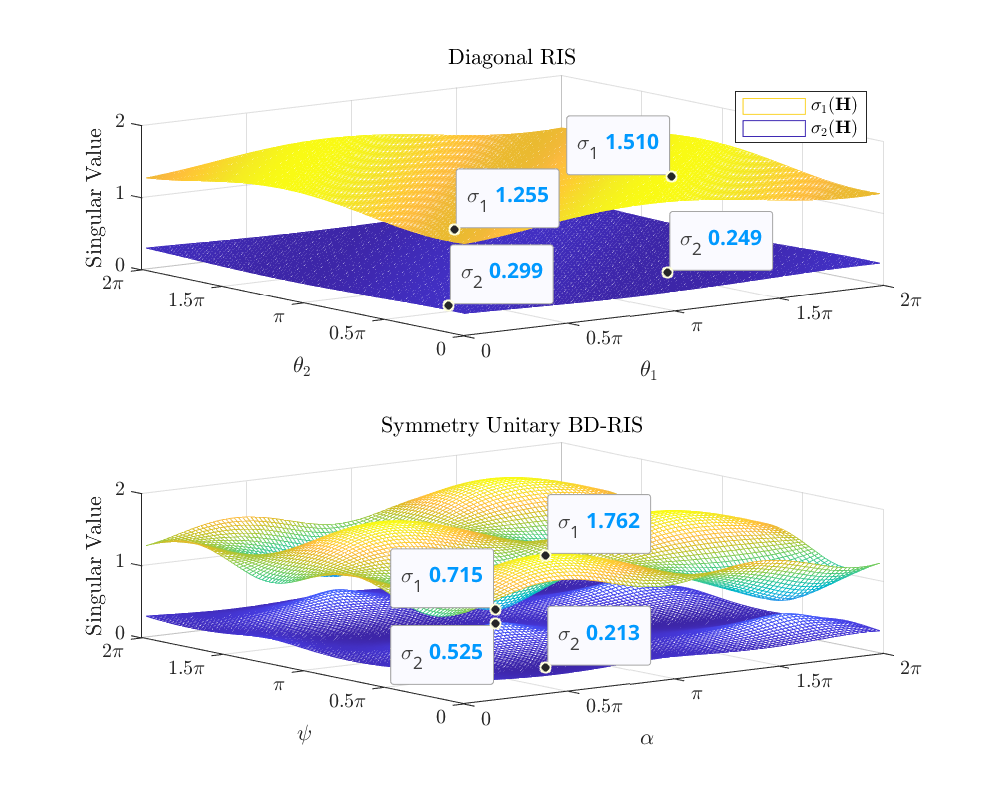
\includegraphics[width=\columnwidth]{assets/simulation/singular_trend.eps}
			\caption{$2 \times 2 \times 2$ (no direct) channel singular value shaping by diagonal and symmetry unitary \gls{ris}.}
			\label{fg:singular_trend}
		\end{figure}
		Fig.~\ref{fg:singular_trend} shows the channel singular values achieved by an exhaustive grid search over $(\theta_1, \theta_2)$ for diagonal \gls{ris} and $(\alpha, \psi)$ for symmetric unitary \gls{ris}.
		It is observed that both singular values can be manipulated up to $9\%$ using diagonal \gls{ris} and $42\%$ using symmetric \gls{bd}-\gls{ris}, despite both architectures have the same number of scattering elements.
		A larger performance gap is expected when the symmetric constraint on \eqref{eq:unitary_ris} can be relaxed.
		This example shows \gls{bd}-\gls{ris} can provide a wider dynamic range of channel singular values and motivates further studies on channel shaping.
	\end{subsection}

	\begin{subsection}{Pareto Frontier Characterization}\label{sc:pareto_frontier}
		We then characterize the Pareto frontier of singular values of a general $N_\mathrm{T} \times N_\mathrm{S} \times N_\mathrm{R}$ channel \eqref{eq:channel_equivalent} by maximizing their weighted sum
		\begin{maxi!}
			{\scriptstyle{\mathbf{\Theta}}}{\sum_n \rho_n \sigma_n(\mathbf{H})}{\label{op:pareto}}{\label{ob:pareto}}
			\addConstraint{\mathbf{\Theta}_g^\mathsf{H} \mathbf{\Theta}_g=\mathbf{I},}{\quad \forall g,}{\label{co:pareto_unitary}}
		\end{maxi!}
		where $n \in \mathcal{N} \triangleq \{1,\ldots,N\}$, $N \triangleq \min(N_\mathrm{T}, N_\mathrm{R})$ is the maximum channel rank, and $\rho_n$ is the weight of the $n$-th singular value that can be positive, zero, or negative.
		Varying $\{\rho_n\}_{n \in \mathcal{N}}$ characterizes the Pareto frontier that encloses the entire achievable singular value region.
		Thus, we claim the singular value Pareto problem \eqref{op:pareto} generalizes most relevant channel shaping problems.
		It can be solved by the proposed group-wise geodesic \gls{rcg} method with the following gradient expression.

		\begin{lemma}\label{lm:pareto_gradient}
			The Euclidean gradient of \eqref{ob:pareto} with respect to \gls{bd}-\gls{ris} group $g$ is
			\begin{equation}
				\frac{\partial \sum_n \rho_n \sigma_n(\mathbf{H})}{\partial \mathbf{\Theta}_g^*} = \mathbf{H}_{\mathrm{B},g}^\mathsf{H} \mathbf{U} \mathrm{diag}(\rho_1,\ldots,\rho_N) \mathbf{V}^\mathsf{H} \mathbf{H}_{\mathrm{F},g}^\mathsf{H},
				\label{eq:pareto_gradient}
			\end{equation}
			where $\mathbf{U}$ and $\mathbf{V}$ are the left and right singular matrices of $\mathbf{H}$, respectively.
		\end{lemma}
		\begin{proof}
			Please refer to Appendix~\ref{ap:pareto_gradient}.
		\end{proof}

		Algorithm~\ref{ag:rcg} can thus be invoked for problem \eqref{op:pareto} where line \ref{ln:gradient_euclidean} uses \eqref{eq:pareto_gradient} explicitly.
		With proper initialization, it is guaranteed to converge to (at least local) optimal points.
	\end{subsection}

	\begin{subsection}{Some Analytical Bounds}\label{sc:bounds}
		We then discuss some analytical bounds related to channel singular values.
		\begin{proposition}[Degree of freedom]\label{pp:dof}
			In point-to-point \gls{mimo}, \gls{bd}-\gls{ris} cannot achieve a higher \gls{dof} than diagonal \gls{ris}.
		\end{proposition}
		\begin{proof}
			Please refer to Appendix~\ref{ap:dof}.
		\end{proof}

		\begin{proposition}[Rank-deficient channel]\label{pp:rank_deficient}
			If the forward or backward channel is rank-$k$ ($k \le N$), then regardless of the passive \gls{ris} size and architecture, the $n$-th singular value of the equivalent channel is bounded by
			\begin{subequations}
				\begin{align}
					\sigma_n(\mathbf{H}) & \le \sigma_{n-k}(\mathbf{T}), &  & \text{if } n > k, \label{iq:sv_bound_enlarge}          \\
					\sigma_n(\mathbf{H}) & \ge \sigma_n(\mathbf{T}),     &  & \text{if } n < N - k + 1, \label{iq:sv_bound_suppress}
				\end{align}
				\label{iq:sv_bound_rank_deficient}
			\end{subequations}
			where
			\begin{equation}
				\mathbf{T} \mathbf{T}^\mathsf{H} =
				\begin{cases}
					\mathbf{H}_\mathrm{D} (\mathbf{I} - \mathbf{V}_\mathrm{F} \mathbf{V}_\mathrm{F}^\mathsf{H}) \mathbf{H}_\mathrm{D}^\mathsf{H}, & \text{if } \mathrm{rank}(\mathbf{H}_\mathrm{F}) = k, \\
					\mathbf{H}_\mathrm{D}^\mathsf{H} (\mathbf{I} - \mathbf{U}_\mathrm{B} \mathbf{U}_\mathrm{B}^\mathsf{H}) \mathbf{H}_\mathrm{D}, & \text{if } \mathrm{rank}(\mathbf{H}_\mathrm{B}) = k,
				\end{cases}
				\label{eq:auxiliary_matrix}
			\end{equation}
			and $\mathbf{V}_\mathrm{F}$ and $\mathbf{U}_\mathrm{B}$ are the right and left compact singular matrices of $\mathbf{H}_\mathrm{F}$ and $\mathbf{H}_\mathrm{B}$, respectively.
		\end{proposition}
		\begin{proof}
			Please refer to Appendix~\ref{ap:rank_deficient}.
		\end{proof}

		\begin{corollary}[Extreme singular values\label{co:extreme}]
			With a sufficiently large passive \gls{ris} of arbitrary architecture, the first $k$ channel singular values are unbounded above\footnote{The energy conservation law $\sum_n \sigma_n^2(\mathbf{H}) \le 1$ still has to be respected. This constraint is omitted in the following context for brevity.} while the last $k$ channel singular values can be suppressed to zero.
		\end{corollary}

		\begin{proof}
			This is a direct result of \eqref{iq:sv_bound_rank_deficient}.
		\end{proof}

		\begin{corollary}[\gls{los} channel\footnote{A similar result has been derived for diagonal \gls{ris} \cite{Semmler2023}.}\label{co:los}]
			% If the forward or backward channel is \gls{los}, then a \gls{ris} can at most enlarge (resp. suppress) the $n$-th ($n \ge 2$) channel singular value to the $(n-1)$-th (resp. $n$-th) singular value of $\mathbf{T}$, that is,
			If the forward or backward channel is \gls{los}, then a passive \gls{ris} of arbitrary architecture can at most enlarge the $n$-th ($n \ge 2$) channel singular value to the $(n-1)$-th singular value of $\mathbf{T}$, or suppress the $n$-th channel singular value to the $n$-th singular value of $\mathbf{T}$.
			That is,
			\begin{equation}
				\sigma_1(\mathbf{H}) \ge \sigma_1(\mathbf{T}) \ge {\sigma_2(\mathbf{H})} \ge \ldots \ge \sigma_{N-1}(\mathbf{T}) \ge {\sigma_N(\mathbf{H})} \ge \sigma_N(\mathbf{T}).
				\label{iq:sv_bound_los}
			\end{equation}
		\end{corollary}

		\begin{proof}
			This is a direct result of \eqref{iq:sv_bound_rank_deficient} with $k = 1$.
		\end{proof}

		In Section~\ref{sc:simulation}, we will show by simulation that a finite-size \gls{bd}-\gls{ris} can better approach those bounds than diagonal \gls{ris}.

		\begin{proposition}[Unitary \gls{ris} without direct link]\label{pp:fully_connected}
			% If the \gls{bd}-\gls{ris} is unitary and the direct link is absent, then the singular value bounds on $\mathbf{H}$ are equivalent to the singular value bounds on $\mathbf{BF}$, where $\mathbf{B}$ and $\mathbf{F}$ are arbitrary matrices with the same singular values as $\mathbf{H}_\mathrm{B}$ and $\mathbf{H}_\mathrm{F}$, respectively,
			If the \gls{bd}-\gls{ris} is unitary and the direct link is absent, then the channel singular values can be manipulated up to
			% If the \gls{bd}-\gls{ris} is unitary and the direct link is absent, then the bounds on the channel singular values are equivalent to the singular values of the equivalent channel, that is,
			% only bounds that apply here are those that apply to the singular values of
			\begin{equation}
				\mathrm{sv}(\mathbf{H}) = \mathrm{sv}(\mathbf{BF}),
			\end{equation}
			where $\mathbf{B}$ and $\mathbf{F}$ are arbitrary matrices with the same singular values as $\mathbf{H}_\mathrm{B}$ and $\mathbf{H}_\mathrm{F}$, respectively,
			% Our focus thus shifts to how the singular values of matrix product are bounded by the singular values of its individual factors.
		\end{proposition}

		\begin{proof}
			Please refer to Appendix~\ref{ap:fully_connected}.
		\end{proof}

		The problem now becomes, how the singular values of matrix product are bounded by the singular values of its individual factors.
		Let $\bar{N} = \max(N_\mathrm{T},N_\mathrm{S},N_\mathrm{R})$ and $\sigma_n(\mathbf{H})=\sigma_n(\mathbf{H}_\mathrm{F})=\sigma_n(\mathbf{H}_\mathrm{B})=0$ for $N < n \le \bar{N}$.
		We have the following corollaries.

		\begin{corollary}[Generic singular value bounds\label{co:sv_bound_horn}]
			\begin{equation}
				\prod_{k \in {K}} \sigma_k(\mathbf{H}) \le \prod_{i \in {I}} \sigma_i(\mathbf{H}_\mathrm{B}) \prod_{j \in {J}} \sigma_j(\mathbf{H}_\mathrm{F}),
				\label{iq:sv_bound_fc}
			\end{equation}
			for all admissible triples $(I, J, K) \in T_r^{\bar{N}}$ with $r < \bar{N}$, where
			\begin{equation*}
				\begin{gathered}
					% T_r^{\bar{N}} \triangleq \Bigl\{(I, J, K) \in U_r^{\bar{N}} \mid \text{for all } p < r \text{ and all } (F, G, H) \text{ in } T_p^r,\\
					% \sum_{f \in F} i_f + \sum_{g \in G} j_g \le \sum_{h \in H} k_h + p(p+1)/2 \Bigr\},
					T_r^{\bar{N}} \triangleq \Bigl\{(I, J, K) \in U_r^{\bar{N}} \mid \forall p < r, (F, G, H) \in T_p^r,\\
					\sum_{f \in F} i_f + \sum_{g \in G} j_g \le \sum_{h \in H} k_h + p(p+1)/2 \Bigr\},
				\end{gathered}
			\end{equation*}
			\begin{equation*}
				U_r^{\bar{N}} \triangleq \Bigl\{(I, J, K) \mid \sum_{i \in I} i + \sum_{j \in J} j = \sum_{k \in K} k + r(r+1)/2\Bigr\}.
			\end{equation*}
		\end{corollary}

		\begin{proof}
			Please refer to \cite[Theorem~8]{Fulton2000}.
		\end{proof}

		Corollary \eqref{co:sv_bound_horn} is by far the most comprehensive singular value bound over Proposition~\ref{pp:fully_connected}, which is also recognized as a variation of Horn's inequality \cite{Bhatia2001}.
		It is worth mentioning that the number of admissible triples (and bounds) grows exponentially with $\bar{N}$.
		For example, the number of inequalities described by \eqref{iq:sv_bound_fc} grows from 12 to 2062 when $\bar{N}$ increases from 3 to 7.
		This renders it computationally expensive for applications in large-scale \gls{mimo} systems.
		Next, we showcase some useful inequalities enclosed by \eqref{iq:sv_bound_fc}.
		Readers are referred to \cite[Chapter 16, 24]{Hogben2013} for more examples.

		\begin{corollary}[Upper bound on the largest singular value\label{co:sv_largest}]
			\begin{equation}
				\sigma_1(\mathbf{H}) \le \sigma_1(\mathbf{H}_\mathrm{B}) \sigma_1(\mathbf{H}_\mathrm{F}).
			\end{equation}
		\end{corollary}

		\begin{proof}
			This is a direct result of \eqref{iq:sv_bound_fc} with $r = 1$.
		\end{proof}

		\begin{corollary}[Lower bound on the smallest singular value\label{co:sv_smallest}]
			\begin{equation}
				\sigma_{\bar{N}}(\mathbf{H}) \ge \sigma_{\bar{N}}(\mathbf{H}_\mathrm{B}) \sigma_{\bar{N}}(\mathbf{H}_\mathrm{F}).
			\end{equation}
		\end{corollary}

		\begin{proof}
			This can be deducted from \eqref{iq:sv_bound_fc} with $r_1 = \bar{N}{-}1$ and $r_2 = \bar{N}$.
		\end{proof}

		\begin{corollary}[Upper bound on the product of first $k$ singular values]
			\begin{equation}
				\prod_{n=1}^k \sigma_n(\mathbf{H}) \le \prod_{n=1}^k \sigma_n(\mathbf{H}_\mathrm{B}) \prod_{n=1}^k \sigma_n(\mathbf{H}_\mathrm{F}).
			\end{equation}
		\end{corollary}

		\begin{proof}
			This is a direct result of \eqref{iq:sv_bound_fc} with $r = k$.
		\end{proof}

		\begin{corollary}[Lower bound on the product of last $k$ singular values\label{co:sv_product_smallest}]
			\begin{equation}
				\prod_{n=\bar{N}}^{\bar{N}-k+1} \sigma_n(\mathbf{H}) \ge \prod_{n=\bar{N}}^{\bar{N}-k+1} \sigma_n(\mathbf{H}_\mathrm{B}) \prod_{n=\bar{N}}^{\bar{N}-k+1} \sigma_n(\mathbf{H}_\mathrm{F}).
			\end{equation}
		\end{corollary}

		\begin{proof}
			This can be deducted from \eqref{iq:sv_bound_fc} with $r_1 = \bar{N}-k$ and $r_2 = \bar{N}$.
		\end{proof}

		Corollaries \ref{co:sv_smallest} and \ref{co:sv_product_smallest} are less informative when $\bar{N} \ne N$ (i.e., unequal number of transmit, scatter, and receive antennas) as the lower bounds would coincide at zero.

		% \begin{corollary}[Upper bound on the sum of first $k$ singular values to the positive $p$-th power\label{co:sum_power} {\cite[Inequality~24.4.7]{Hogben2013}}]
		% 	\begin{equation}
		% 		\sum_{n=1}^k \sigma_n^p(\mathbf{H}) \le \sum_{n=1}^k \sigma_n^p(\mathbf{H}_\mathrm{B}) \sigma_n^p(\mathbf{H}_\mathrm{F}), \quad p > 0.
		% 		\label{iq:sv_bound_fc_power}
		% 	\end{equation}
		% 	When $k = N$ and $p = 2$, \eqref{iq:sv_bound_fc_power} suggests the channel power is upper bounded by the sum of (sorted) element-wise power product of backward and forward subchannels
		% 	\begin{equation}
		% 		\lVert \mathbf{H} \rVert _\mathrm{F}^2 \le \sum_{n=1}^N \sigma_n^2(\mathbf{H}_\mathrm{B}) \sigma_n^2(\mathbf{H}_\mathrm{F}),
		% 	\end{equation}
		% \end{corollary}

		\begin{corollary}[Upper bound on the channel power gain\label{co:sum_power}]
			% The channel power gain is upper bounded by the sum of sorted element-wise power product of backward and forward subchannels
			The channel power gain is upper bounded by the sum of sorted element-wise product of squared singular values of backward and forward subchannels
			\begin{equation}
				\lVert \mathbf{H} \rVert _\mathrm{F}^2 = \sum_{n=1}^N \sigma_n^2(\mathbf{H}) \le \sum_{n=1}^N \sigma_n^2(\mathbf{H}_\mathrm{B}) \sigma_n^2(\mathbf{H}_\mathrm{F}).
				\label{iq:power_gain}
			\end{equation}
		\end{corollary}

		\begin{proof}
			Please refer to \cite[Inequality~24.4.7]{Hogben2013}.
		\end{proof}

		To achieve the equalities in Corollaries \eqref{co:sv_largest} -- \eqref{co:sum_power}, the \gls{ris} needs to completely align the subspaces of $\mathbf{H}_\mathrm{B}$ and $\mathbf{H}_\mathrm{F}$.
		The resulting scattering matrix is generally required to be unitary
		\begin{equation}
			\mathbf{\Theta}^\star = \mathbf{V}_\mathrm{B} \mathbf{U}_\mathrm{F}^\mathsf{H},
			\label{eq:scattering_fc_optimal}
		\end{equation}
		which can be concluded from \eqref{eq:scattering_fc} and \eqref{eq:channel_equivalent_fc} in Appendix~\ref{ap:fully_connected}.
		Interestingly, diagonal \gls{ris} can attain those equalities if and only if $\mathbf{H}_\mathrm{B}$ and $\mathbf{H}_\mathrm{F}$ are both rank-1.
		In such case, the equivalent channel reduces to $\mathbf{H} = \sigma_\mathrm{B} \sigma_\mathrm{F} \mathbf{u}_\mathrm{B} \mathbf{v}_\mathrm{B}^\mathsf{H} \mathbf{\Theta} \mathbf{u}_\mathrm{F} \mathbf{v}_\mathrm{F}^\mathsf{H}$ and the \gls{ris} only needs to align $\mathbf{v}_\mathrm{B}^\mathsf{H}$ and $\mathbf{u}_\mathrm{F}$ by
		\begin{equation}
			\mathbf{\Theta}^\star = \mathbf{v}_\mathrm{B} \mathbf{u}_\mathrm{F}^\mathsf{H} \odot \mathbf{I},
		\end{equation}
		which becomes a special case of \eqref{eq:scattering_siso}.
		On the other hand, when $\mathbf{H}_\mathrm{B}$ and $\mathbf{H}_\mathrm{F}$ are both in Rayleigh fading, the expected maximum channel power gain $\mathbb{E}\bigl\{ \lVert \mathbf{H} \rVert _ \mathrm{F} \bigr\}_{\max}$ can be evaluated as
		\begin{equation}
			\sum_{n=1}^N \int_0^\infty f_{\lambda_n^{\min(N_\mathrm{R},N_\mathrm{S})}}(x_n) d x_n \int_0^\infty f_{\lambda_n^{\min(N_\mathrm{S},N_\mathrm{T})}}(x_n) d x_n,
			\label{eq:power_gain_rayleigh}
		\end{equation}
		where $\lambda_n^{\dot{N}}$ is the $n$-th eigenvalue of the complex $\dot{N} \times \dot{N}$ Wishart matrix with probability density function $f_{\lambda_n^{\dot{N}}}(x_n)$ given by \cite[Equation 51]{Zanella2009}.
		We notice \eqref{eq:power_gain_rayleigh} is a generalization of \cite[Equation 58]{Shen2020a} to \gls{mimo}.

		Tighter bounds are generally inapplicable when the direct link is present or the \gls{bd}-\gls{ris} is not unitary, since the direct-indirect channels and backward-forward channels cannot be completely aligned at the same time.
		In such case, we can exploit optimization approaches from a singular value perspective (Section~\ref{sc:pareto_frontier}) or a power gain perspective (Section~\ref{sc:power}).
	\end{subsection}
\end{section}

\begin{section}{Power Gain and Achievable Rate Maximization}\label{sc:power_rate}
	\begin{subsection}{Channel Power Gain}\label{sc:power}
		The \gls{mimo} channel power gain maximization problem is formulated with respect to the \gls{bd}-\gls{ris} scattering matrix
		\begin{maxi!}
			{\scriptstyle{\mathbf{\Theta}}}{\lVert \mathbf{H}_\mathrm{D} + \mathbf{H}_\mathrm{B} \mathbf{\Theta} \mathbf{H}_\mathrm{F} \rVert _\mathrm{F}^2}{\label{op:power_passive}}{\label{ob:power_passive}}
			\addConstraint{\mathbf{\Theta}_g^\mathsf{H} \mathbf{\Theta}_g=\mathbf{I}, \quad \forall g,}{}{}
		\end{maxi!}
		which generalizes the case of \gls{siso} \cite{Shen2020a}, \gls{miso} \cite{Santamaria2023,Fang2023}, single-stream \gls{mimo} \cite{Nerini2023,Nerini2023b}, and direct-less \gls{mimo} with unitary \gls{ris} \eqref{eq:scattering_fc_optimal}.
		The key of solving \eqref{op:power_passive} is to balance the additive and multiplicative subspace alignments.
		Interestingly, in terms of maximizing the inner product $\langle \mathbf{H}_\mathrm{D}, \mathbf{H}_\mathrm{B} \mathbf{\Theta} \mathbf{H}_\mathrm{F} \rangle$, \eqref{op:power_passive} is reminiscent of the weighted orthogonal Procrustes problem \cite{Gower2004}
		\begin{mini!}
			{\scriptstyle{\mathbf{\Theta}}}{\lVert \mathbf{H}_\mathrm{D} - \mathbf{H}_\mathrm{B} \mathbf{\Theta} \mathbf{H}_\mathrm{F} \rVert _\mathrm{F}^2}{\label{op:weighted_orthogonal_procrustes}}{}
			\addConstraint{\mathbf{\Theta}^\mathsf{H} \mathbf{\Theta}=\mathbf{I},}{\label{cs:power_block_unitary}}{}
		\end{mini!}
		which relaxes the block-unitary constraint \eqref{cs:power_block_unitary} to unitary but still has no trivial solution.
		One lossy transformation exploits the Moore-Penrose inverse and moves $\mathbf{\Theta}$ to one side of the product \cite{Bell2003}, formulating two standard orthogonal Procrustes problems
		\begin{mini!}
			{\scriptstyle{\mathbf{\Theta}}}{\lVert \mathbf{H}_\mathrm{B}^\dagger \mathbf{H}_\mathrm{D} - \mathbf{\Theta} \mathbf{H}_\mathrm{F} \rVert _\mathrm{F}^2 \text{ or } \lVert \mathbf{H}_\mathrm{D} \mathbf{H}_\mathrm{F}^\dagger - \mathbf{H}_\mathrm{B} \mathbf{\Theta} \rVert _\mathrm{F}^2}{\label{op:standard_orthogonal_procrustes}}{}
			\addConstraint{\mathbf{\Theta}^\mathsf{H} \mathbf{\Theta}=\mathbf{I},}{}{}
		\end{mini!}
		which have global optimal solutions
		\begin{equation}
			\mathbf{\Theta} = \mathbf{U} \mathbf{V}^\mathsf{H},
			\label{eq:orthogonal_procrustes_solution}
		\end{equation}
		where $\mathbf{U}$ and $\mathbf{V}$ are respectively the left and right singular matrices of $\mathbf{H}_\mathrm{B}^\dagger \mathbf{H}_\mathrm{D} \mathbf{H}_\mathrm{F}^\mathsf{H}$ or $\mathbf{H}_\mathrm{B}^\mathsf{H} \mathbf{H}_\mathrm{D} \mathbf{H}_\mathrm{F}^\dagger$ \cite{Golub2013}.
		We emphasize that \eqref{eq:scattering_fc_optimal} and \eqref{eq:orthogonal_procrustes_solution} are valid unitary \gls{ris} solutions to \eqref{op:power_passive} when the direct link is absent and present, but the latter is neither optimal nor a generalization of the former due to the lossy transformation.

		Inspired by \cite{Nie2017}, we propose an optimal solution to problem \eqref{op:power_passive} with arbitrary group size.
		The idea is to successively approximate the quadratic objective \eqref{ob:power_passive} by local Taylor expansions and solve each step in closed form by group-wise \gls{svd}.

		\begin{proposition}\label{pp:power}
			Starting from any feasible $\mathbf{\Theta}^{(0)}$, the sequence
			\begin{equation}
				\mathbf{\Theta}_g^{(r+1)} = \mathbf{U}_g^{(r)} \mathbf{V}_g^{(r)}, \quad \forall g.
				\label{eq:scattering_power}
			\end{equation}
			converges to a stationary point of \eqref{op:power_passive}, where $\mathbf{U}_g^{(r)}$ and $\mathbf{V}_g^{(r)}$ are the left and right compact singular matrix of
			\begin{equation}
				\mathbf{M}_g^{(r)} = \mathbf{H}_{\mathrm{B},g}^\mathsf{H} \Bigl(\mathbf{H}_\mathrm{D} + \mathbf{H}_\mathrm{B} \mathrm{diag}\bigl(\mathbf{\Theta}_{[1:g-1]}^{(r+1)},\mathbf{\Theta}_{[g:G]}^{(r)}\bigr) \mathbf{H}_\mathrm{F}\Bigr) \mathbf{H}_{\mathrm{F},g}^\mathsf{H}
				\label{eq:auxiliary_matrix_power}
			\end{equation}
		\end{proposition}

		\begin{proof}
			Please refer to Appendix~\ref{ap:power}.
		\end{proof}
	\end{subsection}

	\begin{subsection}{Achievable Rate Maximization}\label{sc:rate}
		We aim to maximize the achievable rate of the \gls{bd}-\gls{ris}-aided \gls{mimo} system by jointly optimizing the active and passive beamforming
		\begin{maxi!}
			{\scriptstyle{\mathbf{W},\mathbf{\Theta}}}{R = \log \det \biggl(\mathbf{I} + \frac{\mathbf{W}^\mathsf{H}\mathbf{H}^\mathsf{H}\mathbf{H}\mathbf{W}}{\eta}\biggr)}{\label{op:rate}}{\label{ob:rate}}
			\addConstraint{\lVert \mathbf{W} \rVert _\mathrm{F}^2}{\le P}
			\addConstraint{\mathbf{\Theta}_g^\mathsf{H} \mathbf{\Theta}_g}{=\mathbf{I}, \quad \forall g,\label{cs:rate_block_unitary}}
		\end{maxi!}
		where $\mathbf{W}$ is the transmit precoder, $R$ is the achievable rate, $\eta$ is the average noise power, and $P$ is the transmit power constraint.
		Problem \eqref{op:rate} is non-convex due to the block-unitary constraint \eqref{cs:rate_block_unitary} and the coupling between variables.
		We propose a local-optimal approach via \gls{ao} and a low-complexity approach based on channel shaping.

		\begin{subsubsection}{Alternating Optimization}
			This approach updates $\mathbf{\Theta}$ and $\mathbf{W}$ iteratively until convergence.
			For a given $\mathbf{W}$, the passive beamforming subproblem is
			\begin{maxi!}
				{\scriptstyle{\mathbf{\Theta}}}{\log \det \biggl(\mathbf{I} + \frac{\mathbf{H} \mathbf{Q} \mathbf{H}^\mathsf{H}}{\eta}\biggr)}{\label{op:rate_passive}}{\label{ob:rate_passive}}
				\addConstraint{\mathbf{\Theta}_g^\mathsf{H} \mathbf{\Theta}_g=\mathbf{I}, \quad \forall g,}{}{}
			\end{maxi!}
			where $\mathbf{Q} \triangleq \mathbf{W} \mathbf{W}^\mathsf{H}$ is the transmit covariance matrix.
			\begin{lemma}\label{lm:rate_gradient}
				The Euclidean gradient of \eqref{ob:rate_passive} with respect to \gls{bd}-\gls{ris} block $g$ is
				\begin{equation}
					\frac{\partial R}{\partial \mathbf{\Theta}_g^*} = \frac{1}{\eta} \mathbf{H}_{\mathrm{B},g}^\mathsf{H} \biggl(\mathbf{I} + \frac{\mathbf{H}\mathbf{Q}\mathbf{H}^\mathsf{H}}{\eta}\biggr)^{-1} \mathbf{H} \mathbf{Q} \mathbf{H}_{\mathrm{F},g}^\mathsf{H}.
					\label{eq:rate_gradient}
				\end{equation}
			\end{lemma}

			\begin{proof}
				Please refer to Appendix~\ref{ap:rate_gradient}.
			\end{proof}
			Algorithm \ref{ag:rcg} can thus be invoked for problem \eqref{op:rate} where line \ref{ln:gradient_euclidean} uses \eqref{eq:rate_gradient} explicitly.
			Since \eqref{ob:rate_passive} is a concave function of $\mathbf{\Theta}$, convergence to (at least local) optimal points is guaranteed.
			For a given $\mathbf{\Theta}$, the global optimal transmit precoder is given by eigenmode transmission \cite{Clerckx2013}
			\begin{equation}
				\mathbf{W}^\star = \mathbf{V} {\mathrm{diag}(\mathbf{s}^\star)}^{1/2},
				\label{eq:precoder_eigenmode}
			\end{equation}
			where $\mathbf{V}$ is the right singular matrix of the equivalent channel and $\mathbf{s}^\star$ is the optimal water-filling power allocation obtainable by the iterative method \cite{Tse2005}.
			The overall \gls{ao} algorithm is guaranteed to converge to local-optimal points of problem \eqref{op:rate} since each subproblem is solved optimally and the objective is bounded above.
		\end{subsubsection}

		\begin{subsubsection}{Low-Complexity Solution}\label{sc:low_complexity}
			We then propose a suboptimal two-stage solution to problem \eqref{op:rate} that decouples the joint \gls{ris}-transceiver design.
			The idea is to first consider channel shaping and replace the rate maximization problem \eqref{op:rate_passive} by channel power gain maximization problem \eqref{op:power_passive}, then proceed to conventional eigenmode transmission \eqref{eq:precoder_eigenmode}.
			Both steps are solved in closed form and the computational complexity is significantly reduced.
		\end{subsubsection}
	\end{subsection}
\end{section}

\begin{section}{Simulation Results}\label{sc:simulation}
	\begin{table*}[!t]
		\caption{Average Performance of Geodesic and Non-Geodesic \gls{rcg} Algorithms on Problem \eqref{op:pareto}}
		\label{tb:complexity_test}
		\centering
		\begin{tabular}{ccccccc}
			\toprule
			\multirow{2}{*}{\gls{rcg} path} & \multicolumn{3}{c}{$N_\mathrm{S}=16$} & \multicolumn{3}{c}{$N_\mathrm{S}=256$}                                                               \\ \cmidrule(lr){2-4} \cmidrule(lr){5-7}
											& Objective                             & Iterations                             & Time [s]         & Objective        & Iterations & Time [s] \\ \midrule
			Geodesic                        & $\num{4.359e-3}$                      & 11.59                                  & $\num{1.839e-2}$ & $\num{1.163e-2}$ & 25.58      & 3.461    \\
			Non-geodesic                    & $\num{4.329e-3}$                      & 30.92                                  & $\num{5.743e-2}$ & $\num{1.116e-2}$ & 61.40      & 13.50    \\ \bottomrule
		\end{tabular}
	\end{table*}
	In this section, we provide numerical results to evaluate the proposed \gls{bd}-\gls{ris} designs.
	Consider a distance-dependent path loss model $\Lambda(d) = \Lambda_0 d^{-\gamma}$ where $\Lambda_0$ is the reference path loss at distance \qty{1}{m}, $d$ is the propagation distance, and $\gamma$ is the path loss exponent.
	The small-scale fading model is $\mathbf{H} = \sqrt{\kappa/(1+\kappa)} \mathbf{H}_\text{LoS} + \sqrt{1/(1+\kappa)} \mathbf{H}_\text{NLoS}$, where $\kappa$ is the Rician $K$-factor, $\mathbf{H}_\text{LoS}$ is the deterministic \gls{los} component, and $\mathbf{H}_\text{NLoS} \sim \mathcal{CN}(\mathbf{0}, \mathbf{I})$ is the Rayleigh component.
	We set $\Lambda_0=\qty{-30}{dB}$, $d_\mathrm{D}=\qty{14.7}{m}$, $d_\mathrm{F}=\qty{10}{m}$, $d_\mathrm{B}=\qty{6.3}{m}$, $\gamma_\mathrm{D}=3$, $\gamma_\mathrm{F}=2.4$ and $\gamma_\mathrm{B}=2$ for reference, which corresponds to a typical indoor environment with $\Lambda_\mathrm{D}=\qty{-65}{dB}$, $\Lambda_\mathrm{F}=\qty{-54}{dB}$, $\Lambda_\mathrm{B}=\qty{-46}{dB}$.
	The indirect path via \gls{ris} is thus \qty{35}{\dB} weaker than the direct path.
	Rayleigh fading (i.e., $\kappa = 0$) is assumed for all channels unless otherwise specified.

	\begin{subsection}{Algorithm Evaluation}
		We first compare the geodesic and non-geodesic \gls{rcg} algorithm on problem \eqref{op:pareto} in a 4T4R system with \gls{bd}-\gls{ris} group size $L=4$.
		The statistics are averaged over \num{100} independent runs.
		It is observed that the geodesic \gls{rcg} method achieves a slightly higher objective value with significantly (up to 3$\times$) lower number of iterations and shorter (up to 4$\times$) computational time than the non-geodesic method.
		The results demonstrate the efficiency of the proposed geodesic \gls{rcg} algorithm especially in large-scale \gls{bd}-\gls{ris} design problems.
		If the scattering matrix is constrained to be symmetric, one can project the solution to the feasible domain by $\mathbf{\Theta} \gets (\mathbf{\Theta} + \mathbf{\Theta}^\mathsf{T})/2$.
	\end{subsection}

	\begin{subsection}{Channel Singular Values Redistribution}
		\begin{subsubsection}{Pareto Frontier}
			\begin{figure}[!t]
				\centering
				\subfloat[$2 \times 32 \times 2$ (no direct)\label{fg:singular_pareto_sx32_nd}]{
					\resizebox{!}{3.25cm}{
						% This file was created by matlab2tikz.
%
%The latest updates can be retrieved from
%  http://www.mathworks.com/matlabcentral/fileexchange/22022-matlab2tikz-matlab2tikz
%where you can also make suggestions and rate matlab2tikz.
%
\definecolor{mycolor1}{rgb}{0.00000,0.44706,0.74118}%
\definecolor{mycolor2}{rgb}{0.85098,0.32549,0.09804}%
\definecolor{mycolor3}{rgb}{0.92941,0.69412,0.12549}%
\definecolor{mycolor4}{rgb}{0.49412,0.18431,0.55686}%
%
\begin{tikzpicture}

\begin{axis}[%
width=7.607cm,
height=6cm,
at={(0cm,0cm)},
scale only axis,
xmin=0,
xmax=0.00038965048998045,
xlabel style={font=\color{white!15!black}},
xlabel={$\sigma_1$},
ymin=0,
ymax=0.000304493100518335,
ylabel style={font=\color{white!15!black}},
ylabel={$\sigma_2$},
axis background/.style={fill=white},
xmajorgrids,
ymajorgrids,
legend style={at={(0.03,0.97)}, anchor=north west, legend cell align=left, align=left, draw=white!15!black},
every axis plot/.append style={line width=1.5pt}
]
\addplot[only marks, mark=triangle, mark options={}, mark size=2.3570pt, draw=black] table[row sep=crcr]{%
x	y\\
0	0\\
};
\addlegendentry{Direct}

\addplot [color=mycolor1, line width=2.0pt, mark=o, mark options={solid, mycolor1}]
  table[row sep=crcr]{%
0.000267895667198245	0.000171134879393267\\
0.000265726380728974	0.000173150928555956\\
0.000263620365603918	0.000175013140296501\\
0.000261445144530834	0.000176843202895948\\
0.000259164875117885	0.000178667936743009\\
0.000256772775708205	0.000180487719376887\\
0.000254278514486235	0.000182290392662069\\
0.000251704002269913	0.000184056601213238\\
0.000249073506157511	0.000185767894974696\\
0.000246400740748153	0.000187414817948743\\
0.000243687718680905	0.000188995994660418\\
0.000240928492221004	0.000190514582140261\\
0.000238098477127779	0.000191982763893684\\
0.000235165035954025	0.000193414254436945\\
0.000232089995279799	0.000194822374050852\\
0.000228824413086908	0.000196221753795029\\
0.000225316977451163	0.000197623817299328\\
0.000221535346161309	0.000199028850294541\\
0.000203259528520131	0.000203259526698551\\
0.000199827287451323	0.000199827287443645\\
0.000198123535486915	0.000198123535486911\\
0.000180148810088901	0.0001801488100889\\
8.42468741466946e-21	6.05571416226906e-21\\
6.19979890484365e-21	3.35030862543257e-21\\
6.60756407329265e-21	1.28456637898193e-21\\
7.66177135693828e-21	3.92046971006709e-22\\
0.000180096069830613	1.08306169491646e-20\\
0.000191831039008028	1.66189243361953e-20\\
0.000264113777998769	7.79621614858511e-20\\
0.000279564446825807	4.05296860635826e-19\\
0.000280589608744265	1.14924619753218e-18\\
0.000281565424666408	3.19287626893919e-17\\
0.000294887428789775	6.22978162678605e-16\\
0.000298297210243084	1.4033135819947e-15\\
0.000309415141512222	5.02384211049284e-15\\
0.000312286791270632	6.622168556894e-15\\
0.000313941579001134	1.5519784325904e-11\\
0.000315080469539148	2.60442929195929e-06\\
0.000316650462662155	6.20803322481037e-06\\
0.000317953658131026	1.0637150181653e-05\\
0.000319531793152611	1.60801484565072e-05\\
0.000321145121813445	2.39596943662345e-05\\
0.000321463002882309	3.21072961439859e-05\\
0.000321532819016651	3.76429148560442e-05\\
0.000321472892430131	4.25828187614136e-05\\
0.000321300760117647	4.72640647983865e-05\\
0.000321020731972484	5.18237773689732e-05\\
0.000320633271897779	5.63231191746697e-05\\
0.000320137546722193	6.07926465706622e-05\\
0.00031953359137215	6.52391237196603e-05\\
0.000318820183056992	6.96729345667314e-05\\
0.000317997781544904	7.40900801825946e-05\\
0.000317066229794775	7.84903211168037e-05\\
0.000316024782888273	8.28755034268974e-05\\
0.000314867375461116	8.72664954039366e-05\\
0.000313584778992714	9.16888362417147e-05\\
0.000312161323906551	9.61814565544305e-05\\
0.000310588510709343	0.000100752805689686\\
0.000308886100168095	0.000105333037823099\\
0.000307099022755485	0.000109802296733328\\
0.000304874570657941	0.000114975407123897\\
0.000295523412404848	0.000136118926480847\\
0.000293796779560532	0.000139257271731018\\
0.000292107248523008	0.000142157036202118\\
0.000290431849142458	0.000144876663627326\\
0.000288754605499061	0.000147455239474912\\
0.000287064679129902	0.000149918781615647\\
0.000285354493393488	0.000152285164138566\\
0.000283619431704674	0.00015456587543467\\
0.000281858022889306	0.000156766916808042\\
0.000280067185001826	0.00015889544523825\\
0.000278240363912649	0.000160961566094741\\
0.000276367480760894	0.000162977751672099\\
0.000267895667198245	0.000171134879393267\\
};
\addlegendentry{$L = 1$}

\addplot [color=mycolor2, dashed, line width=2.0pt, mark=+, mark options={solid, mycolor2}]
  table[row sep=crcr]{%
0.000355739456151093	0.00023630212231011\\
0.000353983785016404	0.000238013710074763\\
0.000351859225447142	0.000239984970213792\\
0.000349054422291465	0.000242460729759867\\
0.000344270181551168	0.000246471602221089\\
0.000332985328589198	0.000255488751251254\\
0.000326266184355555	0.000260610115544627\\
0.000320562886323912	0.000264733162717323\\
0.000314325700971254	0.000269011913129879\\
0.000308560245761306	0.000272769530149513\\
0.000304688873039902	0.000275159663058865\\
0.000301895314065004	0.000276789729801272\\
0.000299616367457836	0.000278045082584301\\
0.000297629447604807	0.00027907656379607\\
0.000295820894328768	0.000279959625818801\\
0.000294119244751247	0.000280739245424517\\
0.000292480429716739	0.00028144185454148\\
0.000290869271980479	0.000282086202217012\\
0.000289258251330994	0.000282684955608739\\
0.000287439311775594	0.000283221155075434\\
0.000286111329523935	0.000283226241828683\\
0.000281749477516674	0.000281749467335335\\
0.000279440614092202	0.000279440611372918\\
0.000220457825755789	0.000220457825746552\\
0.000208068910616119	0.000208068910610979\\
0.000187946250277845	0.000187946250276701\\
0.000180148810088901	0.000180148810088901\\
6.5591718870255e-05	6.55917188702549e-05\\
4.20164701380515e-21	8.79388127033691e-22\\
6.32472477104445e-21	3.43356879819089e-22\\
0.000175524733181838	4.89153384024627e-21\\
0.000191831039008028	8.05014238109372e-21\\
0.000223156565739869	2.18554354445088e-20\\
0.000298795369668053	4.43259933963327e-19\\
0.000319836197632342	1.14449267159391e-17\\
0.000337395279306117	2.33052717459466e-17\\
0.000345669096124742	1.5235327945565e-16\\
0.000371901015970715	7.29825031398575e-16\\
0.000372437013168705	1.73328225712588e-13\\
0.000372486831885383	2.81023595538404e-05\\
0.000372471466593596	0.000201236641395997\\
0.000372426852724318	0.000202454117307786\\
0.000372354749362613	0.000203628518387191\\
0.000372256427569083	0.000204770528112299\\
0.000372133071603637	0.000205882935186015\\
0.000371985309281415	0.000206970833147438\\
0.000371813719503542	0.000208037182759402\\
0.00037161832382613	0.000209086468304937\\
0.00037139955457068	0.000210119666912738\\
0.00037115668565401	0.000211142180316026\\
0.000370889086656138	0.000212157232410383\\
0.000370596708144513	0.000213165221964369\\
0.000370278106444865	0.000214170692984417\\
0.000369931918553916	0.000215176768360127\\
0.000369557062102171	0.000216184995411197\\
0.000369151325283754	0.000217199302911258\\
0.000368713688516441	0.000218219947660847\\
0.000368241418310008	0.000219250752341472\\
0.000367731914734066	0.000220294367526888\\
0.000367183349266502	0.000221351363599926\\
0.000366591723007183	0.000222425941716797\\
0.000365955230149435	0.00022351770001446\\
0.000365268517707625	0.00022463180272036\\
0.000364529269287204	0.000225767731198768\\
0.000363731076897723	0.000226930750043674\\
0.00036286865154264	0.000228123468496278\\
0.000361936078587719	0.000229348684335404\\
0.000360923096272773	0.000230613841212628\\
0.000359816798832403	0.000231927997905375\\
0.000358602593712985	0.000233300381138745\\
0.000357257858194128	0.000234747077469494\\
0.000355739456151093	0.00023630212231011\\
};
\addlegendentry{$L = 4$}

\addplot [color=mycolor3, dotted, line width=2.0pt, mark=square, mark options={solid, mycolor3}]
  table[row sep=crcr]{%
0.000387644725001034	0.000252163649786122\\
0.000387494244577878	0.000252309874048033\\
0.000387321385451581	0.00025246982456047\\
0.000387123619656507	0.00025264497436984\\
0.000354044414728323	0.000278788391537759\\
0.000324031566213212	0.00030181769538482\\
0.000323370970606122	0.000302322033286758\\
0.000322939503948698	0.000302634503158319\\
0.000322629710522514	0.000302847188929005\\
0.000322389738998535	0.0003030037313976\\
0.000322192012399091	0.000303125657570389\\
0.000322021223310372	0.000303225205191342\\
0.000321868058470525	0.000303309585408043\\
0.000321726332885747	0.00030338319606735\\
0.000321591838228086	0.000303448853401541\\
0.000321461357536437	0.000303508427690401\\
0.000321333801566517	0.000303563282339639\\
0.000321206511969601	0.000303614207600706\\
0.000321078376511536	0.00030366181921831\\
0.000320948398043425	0.00030370654144927\\
0.000320815486892904	0.000303748637788079\\
0.000320678813033656	0.000303788277927965\\
0.000309564989052386	0.000301409733854497\\
0.000288166772576663	0.000287746907546531\\
0.000279440619857278	0.000279440619671027\\
0.000220457825773397	0.000220457825766601\\
0.000193478737274631	0.000193478737273387\\
0.000187946250278386	0.00018794625027787\\
0.000180148810088901	0.000180148810088901\\
7.38779007531488e-05	7.38779007531487e-05\\
6.5591718870255e-05	6.55917188702549e-05\\
6.11855785437379e-21	3.45293064321707e-21\\
4.20164701380515e-21	8.79388127033691e-22\\
1.54145558743596e-20	4.5368881526408e-22\\
0.000121848054411894	4.00695794022811e-21\\
0.000191831039008028	8.05014238109372e-21\\
0.000298795369668053	1.54041673309025e-20\\
0.000319836197632354	2.36457288348854e-18\\
0.000333476889166338	1.75021877124016e-17\\
0.000335729299617477	4.56099183583301e-17\\
0.000337395279306272	8.16975720607573e-17\\
0.000345669096125748	4.1981459702903e-16\\
0.000346031641514439	4.39830021468541e-15\\
0.000387914582890843	1.13358549119329e-12\\
0.000388584823891499	8.0163235518879e-12\\
0.000389055459349451	2.17977036180119e-08\\
0.000389129203196301	2.36054120455867e-05\\
0.000389090206430443	0.000249310691234572\\
0.000389037671865594	0.00024972476835498\\
0.000388990920465773	0.000249934686797231\\
0.000388964382651109	0.000250035016505946\\
0.000388935788614941	0.000250134077714785\\
0.000388905063299093	0.000250231182320069\\
0.000388872172163426	0.000250326693388387\\
0.000388837071247733	0.00025042106587312\\
0.000388799688709563	0.000250514636529308\\
0.000388759882275995	0.000250607325760949\\
0.00038871754306719	0.000250699736848645\\
0.000388672525582172	0.000250792084880618\\
0.000388624572418996	0.000250884495860529\\
0.000388573499339921	0.000250977447103048\\
0.000388518934001622	0.000251071035900666\\
0.000388460497180009	0.000251165596815782\\
0.000388397897277804	0.000251262019216711\\
0.000388330323709399	0.000251359831654839\\
0.000388257446510124	0.0002514612060543\\
0.000388178442275181	0.000251564986042989\\
0.00038809203917229	0.000251672744789679\\
0.000387997416382034	0.000251785310299683\\
0.000387892731864093	0.000251903721206058\\
0.000387776056777691	0.000252029234268639\\
0.000387644725001034	0.000252163649786122\\
};
\addlegendentry{$L = 16$}

\addplot [color=mycolor4, dashdotted, line width=2.0pt, mark=x, mark options={solid, mycolor4}]
  table[row sep=crcr]{%
0.000355261169740309	0.000280320559854823\\
0.00032414018186505	0.000304493100518335\\
0.000324140181659608	0.000304493100483771\\
0.000317179030115277	0.000302551878646465\\
0.000300436107604006	0.000297641691160318\\
0.000220457825791568	0.000220457825777682\\
0.000208068910631096	0.000208068910627274\\
0.000193478737275628	0.000193478737274652\\
0.00018794625027891	0.000187946250278393\\
0.000180148810088901	0.000180148810088901\\
7.38779007531488e-05	7.38779007531487e-05\\
6.71666052516329e-05	6.71666052516328e-05\\
3.15465671181684e-21	1.72642107428799e-21\\
4.53228785082067e-21	7.20639588176322e-22\\
5.64685722791264e-21	5.28482091624286e-22\\
8.20325856378038e-21	1.7761692113009e-22\\
0.000111248475093952	1.37743980728087e-21\\
0.000180096069830613	2.16135335281665e-21\\
0.000298795369668053	5.37505173232332e-21\\
0.000319836197632357	5.46792961128607e-19\\
0.000333476889166367	2.0283151490536e-17\\
0.000337395279306384	5.36077757300478e-17\\
0.000345669096126209	2.78635951089719e-16\\
0.000387914582997111	2.73836722723604e-14\\
0.000389542876653209	2.94230751176389e-08\\
0.000389650489944512	2.36057139085565e-05\\
0.00038965048998045	0.000253270842548633\\
0.000389650489894017	0.000253270843326888\\
0.000355261169740309	0.000280320559854823\\
};
\addlegendentry{$L = 32$}

\addplot[only marks, mark=triangle, mark options={}, mark size=2.3570pt, draw=black] table[row sep=crcr]{%
x	y\\
0	0\\
};
\end{axis}
\end{tikzpicture}%

					}
				}
				\subfloat[$2 \times 32 \times 2$\label{fg:singular_pareto_sx32}]{
					\resizebox{!}{3.25cm}{
						% This file was created by matlab2tikz.
%
%The latest updates can be retrieved from
%  http://www.mathworks.com/matlabcentral/fileexchange/22022-matlab2tikz-matlab2tikz
%where you can also make suggestions and rate matlab2tikz.
%
\definecolor{mycolor1}{rgb}{0.00000,0.44706,0.74118}%
\definecolor{mycolor2}{rgb}{0.85098,0.32549,0.09804}%
\definecolor{mycolor3}{rgb}{0.92941,0.69412,0.12549}%
\definecolor{mycolor4}{rgb}{0.49412,0.18431,0.55686}%
%
\begin{tikzpicture}

\begin{axis}[%
width=7.607cm,
height=6cm,
at={(0cm,0cm)},
scale only axis,
xmin=0.000850130707459294,
xmax=0.001495567105556,
xlabel style={font=\color{white!15!black}},
xlabel={$\sigma_1$},
ymin=5.81124124465135e-05,
ymax=0.000756440229046408,
ylabel style={font=\color{white!15!black}},
ylabel={$\sigma_2$},
axis background/.style={fill=white},
xmajorgrids,
ymajorgrids,
legend style={at={(0.03,0.03)}, anchor=south west, legend cell align=left, align=left, draw=white!15!black},
every axis plot/.append style={line width=1.5pt}
]
\addplot[only marks, mark=triangle, mark options={}, mark size=2.3570pt, draw=black] table[row sep=crcr]{%
x	y\\
0.00117134827739843	0.000407871162732991\\
};
\addlegendentry{Direct}

\addplot [color=mycolor1, line width=2.0pt, mark=o, mark options={solid, mycolor1}]
  table[row sep=crcr]{%
0.00137955431172681	0.000588505616267897\\
0.00137418269622086	0.000593615295742653\\
0.00136749093451528	0.000599376628494274\\
0.00135890213089589	0.000606072077153129\\
0.00134973459427533	0.000612532388777538\\
0.0013410733835681	0.000618021117436472\\
0.00133234723576559	0.000622963402732477\\
0.00132298835416539	0.000627671842535913\\
0.00131283927996255	0.000632167827335414\\
0.00130175068079053	0.000636441315549385\\
0.00128938330235212	0.000640521027244044\\
0.00127272827567336	0.000645071318717164\\
0.001239223656723	0.000652826329399127\\
0.00121181294625974	0.000657515986538869\\
0.0011948709631463	0.000659612394858911\\
0.00117924446441914	0.000660770327164558\\
0.00116465364423377	0.000661132293899478\\
0.00113619330680091	0.000660369140191549\\
0.00111681335066479	0.00065893828544607\\
0.00110400776403201	0.00065738003226823\\
0.00109347165774378	0.000655554479547099\\
0.00108325459149789	0.00065326015322085\\
0.00107295870959626	0.000650409170334344\\
0.00105545417968485	0.000644538951540662\\
0.00104038763128197	0.000638729468304811\\
0.00102417401193919	0.000631551077219278\\
0.00101241548515279	0.000625650365523887\\
0.00100425860502732	0.000621064981892173\\
0.0009940831826727	0.000614742850166296\\
0.000987415602981892	0.000610234296197683\\
0.000980849676409786	0.000605333755974594\\
0.000975257972036462	0.000600727614092169\\
0.000970012018476528	0.000595952796375679\\
0.000965688097012915	0.000591642872687785\\
0.000961613627835618	0.000587170882990767\\
0.000958073981707157	0.000582866103258482\\
0.000954801020084192	0.000578430681164638\\
0.000951712819265589	0.000573772911667256\\
0.000947720748747545	0.000567031466535514\\
0.00094368967956249	0.000559421880095604\\
0.000938666225540191	0.000548842479170087\\
0.000933989675734051	0.000537341214562972\\
0.000929618025042593	0.000524954702892616\\
0.000923396186557418	0.000504608362177913\\
0.000919374605694746	0.000488686430151083\\
0.00091547451826384	0.000469323228217002\\
0.000912531517333292	0.000449138286656906\\
0.000910612071336649	0.000429871807904457\\
0.000909389566483529	0.000408076663647609\\
0.00090933992249972	0.000390775894408823\\
0.000910025743387089	0.000375356272495326\\
0.00091091055269242	0.000366524713164421\\
0.000912645642715888	0.000355223472332591\\
0.000915376017019132	0.000342148360849908\\
0.000919105832897833	0.000327691792510907\\
0.00092356432588294	0.000313121837840753\\
0.000928759465232966	0.000298651133960116\\
0.000942287333852755	0.000265315511165294\\
0.000945407531781455	0.000258678174141125\\
0.000948227552284999	0.000253339610730937\\
0.000951261088922912	0.00024820687902244\\
0.000954330222322886	0.000243539341369861\\
0.000957758218767062	0.000238823590128389\\
0.000960765045145899	0.000235047301644474\\
0.00096247943759114	0.000233103328996495\\
0.000969263161794999	0.000225981910890112\\
0.000977251953109233	0.000218323364932485\\
0.000985528271575816	0.000211536294192776\\
0.000992872848283534	0.000206166024981668\\
0.0010013184827797	0.00020061025405219\\
0.00101013591969619	0.00019539863910245\\
0.00102058684140004	0.000189876058840151\\
0.00103338161892076	0.000183865790027054\\
0.00104875048028412	0.000177484198331724\\
0.00106282584387646	0.00017241993489089\\
0.0010901148768206	0.000164497710367294\\
0.00110349204607487	0.000161179713098831\\
0.00112069218342597	0.00015785505182807\\
0.00113884160166316	0.000155164648932022\\
0.0011562057946585	0.000153460124509895\\
0.00118292823905634	0.000152352333453505\\
0.00120578552949893	0.00015242439366199\\
0.00122445160762688	0.000153374551047328\\
0.00123563402207558	0.000154663630250101\\
0.00124664204314176	0.000156532905506736\\
0.00125646840843924	0.00015873919398177\\
0.0012662380127387	0.000161444101481681\\
0.00127841894557433	0.000165502994603158\\
0.00129598590726039	0.000172188795659219\\
0.00130943172976148	0.000178179258685881\\
0.00132294341473045	0.000184951527100318\\
0.00133349182303189	0.000190922665910368\\
0.0013495725197189	0.000201255032705785\\
0.00136120068833834	0.000209375390277804\\
0.00136890916574433	0.000215378485139867\\
0.00137417862830058	0.000219910697088492\\
0.00137806203541532	0.000223602625444923\\
0.00137806478360425	0.000223605373435129\\
0.00138134703659724	0.000227051007879811\\
0.00138434858265688	0.000230530827225564\\
0.00138726696437118	0.000234272897611889\\
0.00139743637599501	0.000249104704351882\\
0.00140097987249171	0.000254695880160429\\
0.00140427131598064	0.000260507662721602\\
0.0014072558936856	0.000266435943662982\\
0.00140993387764274	0.000272479387021766\\
0.0014125096938205	0.000279170248174948\\
0.00142243876078053	0.000309807745633092\\
0.00142481748232869	0.000318421975031348\\
0.00142751115465991	0.000330552652584366\\
0.00143206701205701	0.000356986980452433\\
0.00143443314590829	0.000376177388259869\\
0.00143628278130165	0.000401042934134447\\
0.00143665815258903	0.000415196865978549\\
0.00143626535833052	0.000429896769863785\\
0.00143475282867046	0.000450519703825262\\
0.00143293009981114	0.00046549066117573\\
0.00143115255664776	0.000475813256555725\\
0.00142892158373648	0.000485645686787124\\
0.00142327161992456	0.000505869693634385\\
0.00141658082101008	0.000525970631421433\\
0.00141195598395635	0.000538042748709412\\
0.00140755516351337	0.000547974537410286\\
0.00140338490443229	0.000556280887626802\\
0.00139978200072969	0.000562651295896027\\
0.00139627232965815	0.000568195828553697\\
0.00139257689630319	0.000573442682146656\\
0.00138859749227567	0.000578540827318686\\
0.00138428272742652	0.000583541389326504\\
0.00137955431172681	0.000588505616267897\\
};
\addlegendentry{$L = 1$}

\addplot [color=mycolor2, dashed, line width=2.0pt, mark=+, mark options={solid, mycolor2}]
  table[row sep=crcr]{%
0.00145175374728852	0.000712138617643247\\
0.00144806552022841	0.000715650077897501\\
0.00144419410443229	0.000718989447528968\\
0.00144013371659298	0.000722157982721491\\
0.00143587610825277	0.000725156273566722\\
0.00143140482272577	0.000727987297831363\\
0.00142670891913738	0.000730646898054616\\
0.00142176925584083	0.000733132631242624\\
0.00141655379316094	0.000735443677233748\\
0.00141103349490505	0.000737572040836793\\
0.00140517129493981	0.000739507419047906\\
0.00139891310187375	0.000741237867860969\\
0.00139220154369391	0.000742743267701533\\
0.00138496439763641	0.000743996938126859\\
0.0013771137514211	0.000744962703532665\\
0.00136853990585377	0.000745592064888499\\
0.00135911155012479	0.000745819620275147\\
0.000934187728827284	0.000745653154728374\\
0.000928012911193149	0.000745200409979498\\
0.000922456865460068	0.000744517424556519\\
0.000917421009822961	0.000743645523110819\\
0.000912832277376057	0.000742616675124022\\
0.000908626350511491	0.00074145409877695\\
0.000904751550943793	0.00074017518558608\\
0.000901167410918195	0.000738793606292529\\
0.000897836762226826	0.000737318079698494\\
0.000894730199791747	0.000735755094341854\\
0.000891821868056294	0.000734108147883148\\
0.000889091406840098	0.000732379592931443\\
0.000886519566943525	0.000730568689085288\\
0.000884716494186002	0.000729172459308234\\
0.000883213275809347	0.000727931011978652\\
0.00088137384608762	0.000726291004326046\\
0.000877105184234858	0.000657669335130148\\
0.000868779169627044	0.000451322305708609\\
0.000859278802721471	0.00020756981136125\\
0.000859216629255504	0.000195032344348207\\
0.00085972887866163	0.000183876743941325\\
0.000860516658984232	0.000175630380822671\\
0.000861632818316307	0.000167793668822133\\
0.00086315707658967	0.000159921188337145\\
0.000864789234581575	0.000153253650498972\\
0.000866811932488616	0.000146491998024455\\
0.00086883762385246	0.000140770733690998\\
0.000871035370689725	0.000135395325402882\\
0.000873393574769313	0.000130333101192121\\
0.000875897055486515	0.000125566912965659\\
0.000878527701202053	0.000121088928592918\\
0.000881385633076845	0.000116720731527713\\
0.000884020893818647	0.0001130770858632\\
0.000886321161444745	0.000110197361051585\\
0.000898351056422359	9.78610012968871e-05\\
0.000901901296192659	9.46800468924414e-05\\
0.000907314830212936	9.0577092539252e-05\\
0.000911918881765063	8.74958718784481e-05\\
0.00091655599180857	8.4726844148044e-05\\
0.000921573148532702	8.20656229455337e-05\\
0.000926196587980724	7.98892038939097e-05\\
0.000931365055731019	7.77424909679372e-05\\
0.000936609977830356	7.58344908886277e-05\\
0.000943587539873934	7.37060966302058e-05\\
0.000950226009355891	7.20523121823955e-05\\
0.000955326860908372	7.10122549005254e-05\\
0.000963072139371514	6.98099915465556e-05\\
0.000969832012280516	6.90544247771336e-05\\
0.000977527091520709	6.85621986428993e-05\\
0.0012130854863295	6.84254518863658e-05\\
0.00141791071928	6.96269161501433e-05\\
0.00142312391154118	7.05296931063686e-05\\
0.00142790940996811	7.16027851071856e-05\\
0.00143232897965355	7.2824540624029e-05\\
0.00143642224036855	7.41756620389875e-05\\
0.0014402317904773	7.56441857939603e-05\\
0.00144378785261983	7.72196357042662e-05\\
0.0014471187471446	7.88955489119111e-05\\
0.00145024686175705	8.06670009665958e-05\\
0.00145319228305501	8.25316293149959e-05\\
0.00145597392620647	8.44902046657583e-05\\
0.0014586063651231	8.65442027981609e-05\\
0.00146110210401823	8.86967904894178e-05\\
0.00146347060971972	9.09516238327398e-05\\
0.00146347270456283	9.09537163181542e-05\\
0.00146572500774135	9.33194750133863e-05\\
0.00146786828031155	9.58043438357939e-05\\
0.00146990747666019	9.84176959452521e-05\\
0.00147184750716623	0.00010117285184622\\
0.00147369058907476	0.000104084138471012\\
0.00147543748873705	0.000107168864311114\\
0.0014770869188056	0.000110447064687982\\
0.00147863604733218	0.000113943643453907\\
0.00148007869334683	0.000117685994871893\\
0.00148140657863155	0.000121708890609374\\
0.0014826071640195	0.000126051874666176\\
0.00148366437255438	0.000130766534909269\\
0.00148455607452328	0.000135916261268162\\
0.00148525193618964	0.000141576944272346\\
0.00148571220804542	0.000147855652949098\\
0.00148588155071661	0.000614577767814696\\
0.00148561238578428	0.00062581568874115\\
0.00148489612765628	0.000635596916778479\\
0.00148383317806433	0.000644248148062585\\
0.00148249253444526	0.000651991901170431\\
0.00148091800089575	0.000659014199832266\\
0.00147913751365726	0.000665454930191529\\
0.00147716830960976	0.000671420239806806\\
0.0014750228946532	0.000676984976134035\\
0.00147270587491031	0.000682214166201574\\
0.00147022084201018	0.000687152535646436\\
0.00146756790409176	0.000691836645914274\\
0.00146474747581704	0.000696291300259663\\
0.0014617564730793	0.000700538627867053\\
0.00145859606643639	0.000704588534607951\\
0.00145526262624861	0.000708453058056901\\
0.00145175374728852	0.000712138617643247\\
};
\addlegendentry{$L = 4$}

\addplot [color=mycolor3, dotted, line width=2.0pt, mark=square, mark options={solid, mycolor3}]
  table[row sep=crcr]{%
0.00149046290152123	0.000749029254155564\\
0.0014900242269345	0.00074944700571706\\
0.00148956595140804	0.000749842385878001\\
0.00148908527851801	0.000750217514822503\\
0.00148858061179832	0.000750572888805431\\
0.00148804928788216	0.00075090929458397\\
0.00148748523631993	0.000751228774981614\\
0.00148688472888253	0.00075153094833365\\
0.00148624325212002	0.000751815163525175\\
0.00148555343341602	0.000752081095560801\\
0.0014848065906605	0.000752327583569775\\
0.00148399652283026	0.00075255146201138\\
0.00148310950182114	0.000752750321984406\\
0.00148213188457328	0.0007529195766878\\
0.00148104571787482	0.000753053088092032\\
0.00147982927991805	0.000753142253382241\\
0.00147845410444853	0.00075317530055406\\
0.000856399484299476	0.000753079955662908\\
0.00085561190314361	0.00075299087227254\\
0.000855168383252795	0.000752894042526675\\
0.000854808259349123	0.000752794560377031\\
0.000854476998753862	0.00075268531896617\\
0.000854171826735235	0.000752567788883797\\
0.000853892942724351	0.000752444475390079\\
0.000853623914142379	0.000752309358535738\\
0.00085337810464549	0.000752170293463684\\
0.000853143937523826	0.00075202220008706\\
0.000852924266392751	0.000751867645258384\\
0.000852713985039399	0.000751703649951764\\
0.000852573654187733	0.000751583253736799\\
0.000852509600662535	0.000751525774234404\\
0.00085216606910422	0.000751009418407836\\
0.000852087035106126	0.00075082980172535\\
0.000851924200217365	0.000750422497451242\\
0.000850371834940363	7.83330461071049e-05\\
0.000850367123973061	7.59963655680903e-05\\
0.000850452392963229	7.44253717148826e-05\\
0.000850572412869088	7.32556626151417e-05\\
0.000850729803715266	7.22122573874861e-05\\
0.000850963683544685	7.10836145599801e-05\\
0.00085117690039885	7.02749238911815e-05\\
0.00085140946312952	6.95414157594678e-05\\
0.000851663484465899	6.88630797042573e-05\\
0.000851921250054968	6.82738127080908e-05\\
0.000852235164654366	6.76406847805733e-05\\
0.00085244098022708	6.72916006764241e-05\\
0.000852575638270119	6.71441261169647e-05\\
0.000855293128156684	6.42194441589772e-05\\
0.000855628679613259	6.39493355269094e-05\\
0.000855976800622717	6.36976812377671e-05\\
0.000856342866396364	6.34551290253909e-05\\
0.00085673172979605	6.32317378177175e-05\\
0.000857371652381497	6.28771846181823e-05\\
0.00085823517243215	6.24998316958764e-05\\
0.000858658557351719	6.23446229182737e-05\\
0.000859302431077715	6.21722239703818e-05\\
0.00086014829123621	6.19824843312733e-05\\
0.000861443678839111	6.1765230282703e-05\\
0.000862185836573078	6.16446201569014e-05\\
0.000865019299296782	6.14668514592799e-05\\
0.00148652830672264	6.24988491252918e-05\\
0.00148756147713045	6.27715119705714e-05\\
0.0014880677690769	6.29637627044874e-05\\
0.00148847364518094	6.31658985332232e-05\\
0.0014889012889211	6.340163880027e-05\\
0.00148958946767849	6.38226172290342e-05\\
0.0014899657954339	6.40859123640802e-05\\
0.00149044958736498	6.44584450088417e-05\\
0.0014907766583995	6.47382107454055e-05\\
0.00149124853041068	6.51802683567342e-05\\
0.00149126387281642	6.51956454924086e-05\\
0.00149162376609705	6.5574211271998e-05\\
0.00149197557836475	6.59824758572283e-05\\
0.00149230879327787	6.64098900092647e-05\\
0.00149270640416903	6.69834976486238e-05\\
0.00149293882889736	6.73543860860554e-05\\
0.00149323394201324	6.78758388121919e-05\\
0.00149351604468895	6.84368795556996e-05\\
0.0014937864155005	6.90478292669155e-05\\
0.00149403855836293	6.97026338361394e-05\\
0.0014942762195696	7.04230012239587e-05\\
0.00149449628185129	7.1219554848062e-05\\
0.00149469367891662	7.21013984572583e-05\\
0.00149486425226757	7.3087028075443e-05\\
0.00149500061683729	7.41978783389704e-05\\
0.00149509793153764	0.000410863543510539\\
0.00149512842708102	0.000734389327803829\\
0.00149508222545898	0.000736322135349975\\
0.00149496077692915	0.000737981317030748\\
0.00149478459564268	0.0007394154266034\\
0.00149456731440495	0.000740671168966442\\
0.0014943182183291	0.000741782777794207\\
0.001494043997576	0.000742775138080022\\
0.00149375005962558	0.000743665850177549\\
0.00149343908306023	0.000744472718100399\\
0.00149311330100405	0.000745208160429862\\
0.00149277399382837	0.000745882586790691\\
0.00149242164900008	0.000746504763466269\\
0.00149205708068219	0.000747080593327281\\
0.00149167950055224	0.000747616787479555\\
0.00149128840330427	0.000748117964075322\\
0.00149088263226683	0.000748588356485789\\
0.00149046290152123	0.000749029254155564\\
};
\addlegendentry{$L = 16$}

\addplot [color=mycolor4, dashdotted, line width=2.0pt, mark=x, mark options={solid, mycolor4}]
  table[row sep=crcr]{%
0.00149386639048453	0.000755049655210065\\
0.00149371321782535	0.000755195521204306\\
0.0014935545341768	0.000755332417443745\\
0.00149338938893506	0.000755461305300265\\
0.00149321694115587	0.000755582756001372\\
0.00149303620516568	0.00075569719649723\\
0.0014928457894547	0.000755805039377688\\
0.00149264498691478	0.000755906076228377\\
0.00149243167931481	0.000756000585561203\\
0.00149220410845542	0.000756088315803518\\
0.00149196000195171	0.000756168891611219\\
0.00149169722763798	0.000756241543642034\\
0.00149141111040051	0.000756305712823123\\
0.0014910979926927	0.00075635991046275\\
0.00149075487766604	0.000756402060862943\\
0.00149037404242127	0.000756429972395182\\
0.00148995046881103	0.000756440229046408\\
0.000850713473664349	0.000756416718845723\\
0.000850663212280196	0.000756406361226111\\
0.000850618768517117	0.000756394757827047\\
0.000850579412502709	0.000756382153355347\\
0.000850543896081195	0.00075636862630528\\
0.000850511372754104	0.000756354265254022\\
0.000850481500978184	0.00075633924846132\\
0.000850453460881014	0.000756323372912526\\
0.000850427409551194	0.000756306881026027\\
0.000850402900072667	0.000756289627563039\\
0.000850379689043704	0.000756271519490907\\
0.000850362461715169	0.000756256819835924\\
0.000850342425569706	0.000756238193485083\\
0.000850130707459294	6.11099280701719e-05\\
0.000850148647025596	6.06874539733784e-05\\
0.000850172021980861	6.04826107331783e-05\\
0.000850196042692511	6.03508340672045e-05\\
0.000850224679739394	6.02346652794101e-05\\
0.000850252156330193	6.01552296980166e-05\\
0.000850927713023346	5.90066160227148e-05\\
0.000851015950565683	5.89088955082686e-05\\
0.000851139093088481	5.87801051186764e-05\\
0.000851355363190468	5.86051095368014e-05\\
0.000851402419252119	5.85682203487598e-05\\
0.000851559198154111	5.84712629153387e-05\\
0.000851614280135624	5.84404156361093e-05\\
0.000851839061286514	5.83251206964467e-05\\
0.000852079176178841	5.82432954935825e-05\\
0.000852544271774776	5.81452091614017e-05\\
0.000853026106262565	5.81124124465135e-05\\
0.00148202778580132	5.87561193247614e-05\\
0.00148995086077685	5.92432048779224e-05\\
0.00149164411536169	5.93937741840165e-05\\
0.00149196951360547	5.9480314746377e-05\\
0.00149257268125237	5.98244890280208e-05\\
0.00149298250414031	6.01503582395203e-05\\
0.00149312170290923	6.02768484821111e-05\\
0.00149360086647569	6.07942590234414e-05\\
0.00149388618441288	6.11328148597379e-05\\
0.00149410150178149	6.14304027310704e-05\\
0.00149413570811437	6.14788441769673e-05\\
0.00149415693008344	6.15102907975543e-05\\
0.00149438279846284	6.18880728895224e-05\\
0.00149467166868244	6.24436727957114e-05\\
0.00149478452214937	6.26982811479396e-05\\
0.0014948113061461	6.27606485455104e-05\\
0.00149495176038534	6.31259618423602e-05\\
0.00149547987929816	0.000410138142976125\\
0.001495567105556	0.000749580677176887\\
0.00149554917810926	0.000750331947706176\\
0.00149550265362032	0.000750967918632245\\
0.00149543511188738	0.000751517850727611\\
0.00149535186555685	0.000751998089470744\\
0.0014952590545945	0.000752411703974411\\
0.00149515652356265	0.000752782740275688\\
0.00149504724871517	0.000753113853451888\\
0.00149493239598821	0.000753411807439089\\
0.00149481287112702	0.00075368157241838\\
0.00149468938022518	0.00075392699028808\\
0.00149456201677617	0.000754151891844859\\
0.00149443084208897	0.000754359097760289\\
0.00149429581983774	0.000754550852231667\\
0.00149415684568532	0.000754728949529443\\
0.00149401388536234	0.000754894698859366\\
0.00149386639048453	0.000755049655210065\\
};
\addlegendentry{$L = 32$}

\end{axis}
\end{tikzpicture}%
					}
				}
				\\
				\subfloat[$2 \times 64 \times 2$\label{fg:singular_pareto_sx64}]{
					\resizebox{!}{3.25cm}{
						% This file was created by matlab2tikz.
%
%The latest updates can be retrieved from
%  http://www.mathworks.com/matlabcentral/fileexchange/22022-matlab2tikz-matlab2tikz
%where you can also make suggestions and rate matlab2tikz.
%
\definecolor{mycolor1}{rgb}{0.00000,0.44706,0.74118}%
\definecolor{mycolor2}{rgb}{0.85098,0.32549,0.09804}%
\definecolor{mycolor3}{rgb}{0.92941,0.69412,0.12549}%
\definecolor{mycolor4}{rgb}{0.49412,0.18431,0.55686}%
%
\begin{tikzpicture}

\begin{axis}[%
width=7.607cm,
height=6cm,
at={(0cm,0cm)},
scale only axis,
xmin=0.000665933747270548,
xmax=0.00180816416675568,
% xlabel style={font=\color{white!15!black}},
xlabel={$\sigma_1(\mathbf{H})$},
ymin=1.10708260774394e-20,
ymax=0.000931271909489233,
% ylabel style={font=\color{white!15!black}},
ylabel={$\sigma_2(\mathbf{H})$},
axis background/.style={fill=white},
xmajorgrids,
ymajorgrids,
legend style={at={(0.03,0.03)}, anchor=south west, legend cell align=left, align=left, draw=white!15!black},
every axis plot/.append style={line width=1.5pt}
]
\addplot[only marks, mark=triangle, mark options={}, mark size=2.3570pt, draw=black] table[row sep=crcr]{%
x	y\\
0.00123451554249979	0.000261671419241521\\
};
\addlegendentry{Direct}

\addplot [color=mycolor1, line width=2.0pt, mark=o, mark options={solid, mycolor1}]
  table[row sep=crcr]{%
0.00159608285697502	0.000664114392083429\\
0.00158691664294714	0.000672837941128764\\
0.00157660050010728	0.000681731690268777\\
0.00156590259762528	0.000690085825238813\\
0.00155467994239563	0.000697976645701225\\
0.00153986973643909	0.000707372645028292\\
0.0015148645023757	0.000721449433364078\\
0.00149697676532785	0.000730394195338623\\
0.0014811063630021	0.000737471285391353\\
0.00146705261153674	0.000742888836825103\\
0.00145145312317651	0.000748034879132762\\
0.00143354032724506	0.000752981116885134\\
0.00141219815168891	0.00075775662502572\\
0.00138599656893751	0.000762282978521517\\
0.001355981991655	0.00076597328234428\\
0.00132155867810352	0.000768494850647513\\
0.00127159845792326	0.000769595351798804\\
0.00123642786506839	0.000768807421978087\\
0.00121422536014095	0.000767187754726459\\
0.00118743020096022	0.000763797105859703\\
0.00116236115681128	0.000759517337937116\\
0.00114216255507682	0.000754981192412643\\
0.00112132876332356	0.000749208839458789\\
0.0010987179355452	0.000741727590503771\\
0.001073267755154	0.000731896088791152\\
0.00104840588147425	0.00072089161304077\\
0.00103123882758884	0.000712332026035008\\
0.00102072542642717	0.00070661151546976\\
0.00101127064407598	0.000700865695981975\\
0.00100290573808909	0.000695274516366674\\
0.00099405869556404	0.000688750411001148\\
0.000985723184951612	0.000681989259163176\\
0.000977942269806648	0.000675005939163037\\
0.000883365237789003	0.000578594721583551\\
0.000875259823033198	0.000568804316998415\\
0.00086636420891398	0.000556929660283238\\
0.000858029700529914	0.000544803768004766\\
0.000849145080144272	0.00053057937604649\\
0.000840385049788102	0.00051511967478722\\
0.000831240490517266	0.000497160206301654\\
0.000823405081875965	0.000479893545133291\\
0.000814633564461672	0.000458113314889421\\
0.000806977608550476	0.000436163726292382\\
0.000800072243550595	0.000412970991852368\\
0.000793559072159092	0.000386530995276439\\
0.000788411273090975	0.000360210129693543\\
0.000784467319171457	0.000332879132259079\\
0.000781370109809877	0.000300494465576911\\
0.000779229604973693	0.000255973167522945\\
0.000778843765690314	0.000189061764117299\\
0.000780851644081482	0.00014653579410713\\
0.00078386863842555	0.000116085317999348\\
0.000787435958310619	9.41678760729649e-05\\
0.00079298844062422	6.9432611338902e-05\\
0.000797722113984264	5.34238131636791e-05\\
0.000802073424201546	4.09329153574363e-05\\
0.000806203726326662	3.06917584825308e-05\\
0.000813014934977753	2.20160208093019e-05\\
0.000824950988932121	7.10447651041556e-06\\
0.000827696888811626	3.85134078631187e-06\\
0.000830547864235395	1.21674953920938e-06\\
0.000831965275229041	2.44617826405831e-07\\
0.000832649165431366	1.79133867425279e-08\\
0.000832828850348146	1.10708260774394e-20\\
0.00161378237741308	6.65749607101577e-19\\
0.00161378237741355	5.8393880144134e-16\\
0.00161378237849435	1.32872382628457e-12\\
0.00161639227547958	3.40455067607412e-06\\
0.00163014580907626	2.28971513147335e-05\\
0.00163990293192521	3.82518884070967e-05\\
0.00164673659382605	5.02988168914937e-05\\
0.00165256368270938	6.18735109090836e-05\\
0.00165770600095059	7.34703347459089e-05\\
0.00166401148822954	8.99928952340316e-05\\
0.00167059283856931	0.000109936635373391\\
0.00167658908453108	0.00013162628400113\\
0.00168183527674099	0.000155018775367617\\
0.00168631721115301	0.000180982050508911\\
0.00169157776515169	0.000222197499567037\\
0.0016938416476388	0.000253372151620205\\
0.00169524815187732	0.000327486553761353\\
0.00169398163691352	0.000384104665758756\\
0.00169113344593976	0.000423595412164682\\
0.00168746779562959	0.00045341619951097\\
0.00168166868784352	0.000486331065994069\\
0.00167573939279825	0.000513052824819554\\
0.00166982471571825	0.000534440995798568\\
0.00166328466709128	0.000554261223027059\\
0.00165659661416354	0.000571625272087831\\
0.00164994826526868	0.00058664202350194\\
0.00164324082244803	0.000599976257139259\\
0.00163623992074054	0.000612337398149498\\
0.00162880459408019	0.00062408033199365\\
0.00162098454625344	0.000635186241435433\\
0.00161290650953524	0.00064554019696715\\
0.00160463337370114	0.000655133158519538\\
0.00159608285697502	0.000664114392083429\\
};
\addlegendentry{$L = 1$}

\addplot [color=mycolor2, dashed, line width=2.0pt, mark=+, mark options={solid, mycolor2}]
  table[row sep=crcr]{%
0.0017386594129955	0.000860048272090083\\
0.00173620516066716	0.000862385276306713\\
0.00173365845469748	0.000864582194303698\\
0.00173100324095088	0.000866654293858911\\
0.00172822270935142	0.000868612367139377\\
0.00172529641442896	0.000870465091689542\\
0.00172219949784328	0.000872218997274339\\
0.00171890327802487	0.000873877536139426\\
0.00171537346710331	0.000875441416860692\\
0.00171156313466259	0.00087691025673575\\
0.00170742153093652	0.000878277201093898\\
0.00170288236322903	0.00087953179778277\\
0.00169786056348726	0.000880657548119832\\
0.00169224883215724	0.000881628811261486\\
0.00168591886705108	0.000882406429632005\\
0.00167869706302702	0.000882935175885586\\
0.00167037980039834	0.000883134115394112\\
0.00102052209736536	0.000882801692620656\\
0.00101646047276367	0.000882503284497043\\
0.00101267238345347	0.000882037044403964\\
0.00100912045073618	0.000881421520159389\\
0.00100577415829649	0.000880670753564986\\
0.00100260461810987	0.000879794177847139\\
0.000999591303638097	0.00087879914985014\\
0.000996714501147741	0.000877689800195453\\
0.000993956695076467	0.000876467622492497\\
0.000991304163226718	0.000875132632656254\\
0.00098874401757588	0.000873682418028017\\
0.00098626581874889	0.000872113116072078\\
0.000983859443434805	0.000870418263617197\\
0.000982667940276653	0.000869508063587063\\
0.000980791270287472	0.00086797495643917\\
0.000978764853396329	0.000866174303123083\\
0.00073858103322915	0.000625587747554838\\
0.000736804562629995	0.00062341605253277\\
0.000735216509742291	0.000621195965101899\\
0.000733326042401016	0.000618190330161238\\
0.000731462763390808	0.000614635580866718\\
0.00072960197688474	0.000610261186413097\\
0.000727481471851482	0.000604194613646108\\
0.000725774643635242	0.00059698869144714\\
0.000724411832896014	0.000588243050464741\\
0.000722671507844784	0.00057242143535709\\
0.000720908493707654	0.000551316307025198\\
0.000717663020121559	0.000480820238180472\\
0.00071027146682115	1.85577797620156e-07\\
0.000710272133741029	2.04326485221653e-20\\
0.000710272133741029	1.24468938843598e-20\\
0.00176612080949286	4.10800016469333e-20\\
0.00176612080949286	1.85966565899392e-18\\
0.00176612080954112	1.05266522974633e-12\\
0.00176658705241273	0.000768319728234086\\
0.00176627636802428	0.000781399086076133\\
0.001765475267997	0.000792357337836094\\
0.00176432796955949	0.000801704108891192\\
0.00176293138974357	0.000809777996388858\\
0.00176135178909172	0.000816827834029172\\
0.00175963734811238	0.000823033257292548\\
0.00175782002453809	0.000828541533511611\\
0.00175592216240292	0.000833466677211746\\
0.00175395850137951	0.000837900348712894\\
0.00175193781323402	0.000841917498031388\\
0.00174986495888347	0.000845578643152257\\
0.0017477395215548	0.000848936553024065\\
0.00174556170527002	0.000852029858633396\\
0.00174332601024846	0.000854895377084003\\
0.00174102703287014	0.000857561023545491\\
0.0017386594129955	0.000860048272090083\\
};
\addlegendentry{$L = 4$}

\addplot [color=mycolor3, dotted, line width=2.0pt, mark=square, mark options={solid, mycolor3}]
  table[row sep=crcr]{%
0.00179380276845171	0.00091689979762741\\
0.00179330381640944	0.000917374896950445\\
0.00179278266048231	0.000917824483975737\\
0.00179223588641608	0.000918251208265826\\
0.00179166118529593	0.00091865597284368\\
0.00179105243790838	0.000919041439304825\\
0.00179040687137795	0.000919407052815547\\
0.00178971966764065	0.000919752827018602\\
0.00178898345155905	0.000920079015279063\\
0.00178819041326094	0.000920384737764874\\
0.00178733064593907	0.000920668516231091\\
0.00178639456888193	0.000920927244200767\\
0.00178536783735916	0.000921157441801043\\
0.0017842320969085	0.000921354081194788\\
0.00178296621498302	0.000921509663813811\\
0.00178154397059403	0.000921613885204562\\
0.0017799292148076	0.000921652660192432\\
0.000988173389737295	0.000921582699284711\\
0.000957736273207751	0.000921529495829503\\
0.000956956181711174	0.000921436401691889\\
0.000956262822922715	0.000921316245628706\\
0.000955621424562645	0.000921172308373418\\
0.000955026459647334	0.000921007721403984\\
0.000954469354603954	0.000920823719947534\\
0.000953946831222138	0.000920622178674876\\
0.00095345140828616	0.000920402549695003\\
0.000952983758568837	0.000920167088503862\\
0.000952538188648702	0.000919914641645634\\
0.000952111090952238	0.000919644150536898\\
0.000951701194433098	0.000919355407751773\\
0.000951305944643583	0.000919046852318652\\
0.000950925140027922	0.000918718263904203\\
0.000950848596271687	0.000918647407418934\\
0.000679717985371998	0.000646470303425183\\
0.000679378897894892	0.000645792824605016\\
0.000679064490109163	0.000645032778423549\\
0.000678722747899459	0.000644083164721458\\
0.000677914453470986	0.000641232357239559\\
0.00067750701005809	0.000638207934222391\\
0.000677322919355633	0.000635620156515246\\
0.000677047863285968	0.000630803033852765\\
0.000674975974668598	5.06904442744669e-08\\
0.000674977394216685	2.27657807105469e-20\\
0.000674977394217525	2.0914813109004e-20\\
0.00179895941878977	5.27490978356368e-16\\
0.00179895941879047	2.50903236847347e-14\\
0.00179895941879441	3.04019292668737e-13\\
0.00179895941880352	1.03827816531674e-12\\
0.00179895941881027	1.59019368378821e-12\\
0.00179895941882359	3.20186569698865e-12\\
0.00179895941884063	5.63352168589419e-12\\
0.0017991011722443	0.000900190223937653\\
0.00179904761519291	0.000902434408333122\\
0.00179890811245153	0.000904341359869694\\
0.00179870656384648	0.000905983094296771\\
0.00179845843443343	0.00090741758790198\\
0.00179817474211808	0.00090868352751566\\
0.00179786315604028	0.000909810873569764\\
0.00179752971313305	0.000910821053531535\\
0.00179717732419367	0.000911735177535424\\
0.00179680876466913	0.000912567112422704\\
0.00179642418724526	0.000913331493190543\\
0.0017960252855648	0.000914035854842987\\
0.00179561177040327	0.000914688958760955\\
0.00179518419519686	0.000915296119290815\\
0.00179474074215017	0.000915864399173621\\
0.00179428054460277	0.000916397925030764\\
0.00179380276845171	0.00091689979762741\\
};
\addlegendentry{$L = 16$}

\addplot [color=mycolor4, dashdotted, line width=2.0pt, mark=x, mark options={solid, mycolor4}]
  table[row sep=crcr]{%
0.00180555185284818	0.000929399946939874\\
0.00180533514986291	0.000929606320188223\\
0.00180511241911368	0.000929798491198706\\
0.00180488301833069	0.000929977560540128\\
0.00180464543585704	0.000930144931618639\\
0.00180439887046556	0.000930301114559859\\
0.00180414061727167	0.000930447428205666\\
0.00180387197745908	0.000930582648819448\\
0.00180358777824979	0.000930708610274962\\
0.00180328851982513	0.0009308239951381\\
0.00180297041976148	0.000930929010172791\\
0.00180263140440767	0.000931022740000879\\
0.00180226747773386	0.000931104368117137\\
0.00180187450841429	0.000931172452949046\\
0.00180144635722952	0.000931225124403758\\
0.00180097831933697	0.000931259464153654\\
0.00180046348509318	0.000931271909489233\\
0.000944849900941658	0.000931211694645889\\
0.000944839913505128	0.000931209338074817\\
0.00094483470026005	0.000931207092411984\\
0.00094483124185063	0.000931205333770562\\
0.000944828626165158	0.000931203830760087\\
0.00094482570824285	0.000931201962340366\\
0.000944823320857996	0.000931200264243388\\
0.000944820797083095	0.000931198282524072\\
0.000944818436457118	0.000931196231738259\\
0.000944817065599912	0.000931194940775414\\
0.000666172865144616	0.000641827260687818\\
0.00066608480570714	0.000641225162002834\\
0.000665933747270548	5.1429931679751e-09\\
0.000665937663943505	2.6464573050457e-18\\
0.000665937663957412	2.56331862610015e-20\\
0.00179284167343554	4.12442654237233e-14\\
0.00179996213281698	0.000131597351506554\\
0.00180741613556227	0.000385954778968086\\
0.00180816416675568	0.00092051863831523\\
0.00180813232064453	0.000921859200902388\\
0.00180805141427027	0.000922966363355986\\
0.00180793735194591	0.000923896258342538\\
0.00180780005090852	0.000924690490277386\\
0.00180764709754446	0.000925373483790865\\
0.00180748259104349	0.000925969298705207\\
0.00180730920132486	0.000926495018121581\\
0.00180712977427	0.000926960625605547\\
0.00180694604044497	0.000927375443789162\\
0.00180675764720281	0.000927749950181251\\
0.00180656608987988	0.00092808825455196\\
0.00180637080873473	0.000928396761518694\\
0.00180617226146695	0.000928678778348136\\
0.00180596971317736	0.000928938408687284\\
0.00180576306092541	0.000929178045128876\\
0.00180555185284818	0.000929399946939874\\
};
\addlegendentry{$L = 64$}

\end{axis}
\end{tikzpicture}%

					}
				}
				\subfloat[$2 \times 128 \times 2$\label{fg:singular_pareto_sx128}]{
					\resizebox{!}{3.25cm}{
						% This file was created by matlab2tikz.
%
%The latest updates can be retrieved from
%  http://www.mathworks.com/matlabcentral/fileexchange/22022-matlab2tikz-matlab2tikz
%where you can also make suggestions and rate matlab2tikz.
%
\definecolor{mycolor1}{rgb}{0.00000,0.44706,0.74118}%
\definecolor{mycolor2}{rgb}{0.85098,0.32549,0.09804}%
\definecolor{mycolor3}{rgb}{0.92941,0.69412,0.12549}%
\definecolor{mycolor4}{rgb}{0.49412,0.18431,0.55686}%
%
\begin{tikzpicture}

\begin{axis}[%
width=7.607cm,
height=6cm,
at={(0cm,0cm)},
scale only axis,
xmin=6.82872585627327e-18,
xmax=0.00243816160662188,
% xlabel style={font=\color{white!15!black}},
xlabel={$\sigma_1(\mathbf{H})$},
ymin=3.65485567546015e-21,
ymax=0.00161848476949908,
% ylabel style={font=\color{white!15!black}},
ylabel={$\sigma_2(\mathbf{H})$},
axis background/.style={fill=white},
xmajorgrids,
ymajorgrids,
legend style={at={(0.03,0.97)}, anchor=north west, legend cell align=left, align=left, draw=white!15!black},
every axis plot/.append style={line width=1.5pt}
]
\addplot[only marks, mark=triangle, mark options={}, mark size=2.3570pt, draw=black] table[row sep=crcr]{%
x	y\\
0.00106823197271749	0.000315419858965939\\
};
\addlegendentry{Direct}

\addplot [color=mycolor1, line width=2.0pt, mark=o, mark options={solid, mycolor1}]
  table[row sep=crcr]{%
0.00184667263255644	0.00105283104259383\\
0.00182013858730192	0.00107811414263772\\
0.00179446438717075	0.00110027146645747\\
0.00176844990466793	0.00112057240647327\\
0.00174471598225592	0.00113735225073209\\
0.00173147018986277	0.0011457366537772\\
0.00171580206722167	0.00115459255032051\\
0.00169703638968541	0.00116404598160524\\
0.00167988551784587	0.00117165264042197\\
0.00165718151718767	0.00118033305141772\\
0.00163702803533105	0.00118700156329319\\
0.00161226798692668	0.00119381007407023\\
0.00157105208627055	0.00120298087682078\\
0.00150917948363715	0.00121387316714933\\
0.00147157873771745	0.00121848599716562\\
0.00141343882647389	0.00122268663375429\\
0.00135084809104336	0.00122423429959488\\
0.00128936609099569	0.00122271750802284\\
0.00121973809357671	0.00121765733083521\\
0.00121741694180727	0.00121741694049506\\
0.00121741694033254	0.00121741694033254\\
0.00121741694033254	0.00121741694033254\\
0.000119403095894786	0.000119403095894786\\
0.000119403095894786	0.000119403095894786\\
0.000119403095894786	0.000119403095894785\\
0.000119403095868481	0.000119403095619605\\
0.000119403020394798	0.000119402298841366\\
0.000119386835029527	0.000119220988146345\\
0.000119057519576339	0.000114537334043434\\
0.000118455254948543	9.74254158896766e-05\\
0.000118475403377689	6.05430449574898e-05\\
0.000119625289046176	3.58679417568317e-05\\
0.000121423832495273	1.68770395478336e-05\\
0.000123412343773753	3.63936799619954e-06\\
0.000126000066494017	2.66928867246076e-10\\
0.000126094125790575	7.84463000637013e-16\\
0.000126164157534685	1.20407546614755e-19\\
0.000126171645826149	1.34875575902017e-20\\
0.000464871894092027	3.07637746131283e-20\\
0.00212946194498699	1.28942837838959e-19\\
0.00212946194498699	6.05180410022353e-19\\
0.00213171673459533	1.04876633850556e-05\\
0.00213642096799013	3.76095271630723e-05\\
0.00214246905743812	8.74587445329254e-05\\
0.00214751768540749	0.000157066053816262\\
0.00215085610784843	0.000271599925869964\\
0.00214933836456014	0.00033572935755316\\
0.00214495278417729	0.000395001725460926\\
0.00213813677099238	0.000450421310742063\\
0.00212769108455725	0.000510559965583877\\
0.0021139023007005	0.000571766564918572\\
0.00209785728241506	0.000629897607970685\\
0.00208118843029345	0.000680330658337416\\
0.00206298961265576	0.000727725985644975\\
0.00204487386350509	0.000768568135802446\\
0.0020225203667261	0.000812913003034874\\
0.00199616218047092	0.000859421583248756\\
0.0019661374861644	0.000906979746165971\\
0.00193991813992618	0.000944225376108491\\
0.00191015036907694	0.000982312334340278\\
0.00187569450797794	0.00102229903484787\\
0.00184667263255644	0.00105283104259383\\
};
\addlegendentry{$L = 1$}

\addplot [color=mycolor2, dashed, line width=2.0pt, mark=+, mark options={solid, mycolor2}]
  table[row sep=crcr]{%
0.00224810954787343	0.00142765882888639\\
0.00223752516987624	0.00143773668940813\\
0.00222645577942414	0.00144728533430297\\
0.00221483758007418	0.00145635192562367\\
0.0022025971723238	0.00146497167929375\\
0.00218964306727519	0.00147317316537416\\
0.0021758697346165	0.00148097339279209\\
0.00216113623435137	0.00148838676976667\\
0.00214526641585671	0.00149541773160406\\
0.00212805031445442	0.00150205397827131\\
0.00210921569109828	0.00150827010338685\\
0.00208840018900012	0.00151402285650014\\
0.00206515213082401	0.00151923352023128\\
0.00204653673297032	0.00152250712144237\\
0.0020319724883019	0.00152429677367295\\
0.00201538660022458	0.00152551134991323\\
0.00199610708059676	0.00152597176892137\\
0.00152539239259048	0.0015253923826303\\
0.00152539238261993	0.00152539238223587\\
0.00152539238222263	0.00152539238221814\\
0.00152539238221792	0.00152539238221792\\
2.5656190712798e-05	2.56561907127979e-05\\
2.5656190712798e-05	2.56561907127979e-05\\
2.56542030161616e-05	2.55564221517753e-05\\
2.55651332386643e-05	1.80765962966132e-05\\
2.54274242107853e-05	3.89478936932254e-08\\
2.54284933602812e-05	9.88017767029914e-20\\
2.54284933602812e-05	3.65485567546015e-21\\
0.00235185136612809	1.88970490505015e-19\\
0.00235185136612809	1.89904129212748e-19\\
0.00235185136623601	2.10937246606743e-12\\
0.00235306574672104	0.00112241590476244\\
0.00235222900963638	0.00115749997958599\\
0.00234998758195604	0.00118808242566059\\
0.00234662460486239	0.00121543787151824\\
0.00234233285079524	0.00124022235534106\\
0.00233725320120539	0.00126287502712395\\
0.00233149354254889	0.0012837093862117\\
0.00232513727045498	0.00130296539740488\\
0.00231825051346261	0.00132082977484434\\
0.00231088706115753	0.00133744986558083\\
0.00230308575053904	0.00135295487223089\\
0.00229487765359623	0.00136744900965217\\
0.00228628461857372	0.00138102243969255\\
0.00227731644465318	0.00139375886428586\\
0.00226797184875481	0.0014057346459718\\
0.00225824024199718	0.00141701733112661\\
0.00224810954787343	0.00142765882888639\\
};
\addlegendentry{$L = 4$}

\addplot [color=mycolor3, dotted, line width=2.0pt, mark=square, mark options={solid, mycolor3}]
  table[row sep=crcr]{%
0.00238467756794191	0.00157463743802116\\
0.0023819055258318	0.00157727655066139\\
0.00237896534516425	0.00157981282300349\\
0.00237584496745458	0.00158224793554099\\
0.00237252341665759	0.00158458699447776\\
0.00236898096929058	0.00158682982530082\\
0.00236518489959242	0.00158897971725607\\
0.00236110787568849	0.00159103122832968\\
0.00235670400375528	0.0015929825465803\\
0.00235192681387114	0.00159482430984728\\
0.00234671740987606	0.00159654394608101\\
0.00234101372325919	0.00159812080273434\\
0.00233471410748323	0.00159953351436297\\
0.0023277213879351	0.00160074429522783\\
0.00231990369916102	0.00160170525428858\\
0.00231109266365087	0.00160235119567967\\
0.00230106518932941	0.00160259231647374\\
0.00160118657134884	0.00160118657130681\\
0.00160118657130541	0.00160118657130541\\
0.00160118657130541	0.00160118657130541\\
6.82872585627327e-18	6.74276093779542e-18\\
6.88479121295111e-18	6.56284337752166e-18\\
7.42057943416505e-18	5.97949898675849e-18\\
1.02652588277888e-17	2.97624528851796e-18\\
1.35225160295751e-17	9.81653158908711e-19\\
4.14744432044337e-17	2.45169228672175e-20\\
7.31026945953357e-17	1.12901305223653e-20\\
0.00240962077068218	8.49382046082521e-20\\
0.00240962077068218	7.13445152076569e-19\\
0.00240962077068218	1.82769532418166e-15\\
0.00240962077068223	3.61308205942841e-14\\
0.00241036864849235	0.000689895899012993\\
0.00241058391784397	0.001500391286991\\
0.00241038337686835	0.00150873726156622\\
0.0024098417777718	0.00151612468860024\\
0.00240902820374127	0.00152274239623327\\
0.00240799204744864	0.00152872601777691\\
0.00240676935813045	0.00153417843028343\\
0.00240538530850182	0.0015391847600932\\
0.00240385837864775	0.00154381019963698\\
0.00240220130519937	0.00154810819989861\\
0.00240042398682364	0.00155211931244551\\
0.00239852970644693	0.00155588372037528\\
0.00239652119195967	0.0015594299630115\\
0.00239439821373247	0.00156278291878547\\
0.0023921563985175	0.00156596608984207\\
0.00238979468829576	0.0015689920967447\\
0.0023873042623312	0.00157187887211322\\
0.00238467756794191	0.00157463743802116\\
};
\addlegendentry{$L = 16$}

\addplot [color=mycolor4, dashdotted, line width=2.0pt, mark=x, mark options={solid, mycolor4}]
  table[row sep=crcr]{%
0.00243247601307818	0.00161102948034108\\
0.00243181726442887	0.00161165656477936\\
0.00243111150394324	0.0016122652276857\\
0.00243034895492804	0.00161286020159992\\
0.00242952456255834	0.00161344066443583\\
0.00242862742029526	0.001614008619057\\
0.00242764675719739	0.00161456392365131\\
0.00242657046026066	0.00161510534481505\\
0.0024253816348233	0.00161563184601292\\
0.00242406462370524	0.00161613934041111\\
0.00242258868646807	0.00161662631813364\\
0.00242092561566571	0.00161708574928453\\
0.00241903974380994	0.0016175082481848\\
0.00241688060323457	0.00161788176032039\\
0.00241438047713464	0.00161818872597477\\
0.00241145950912255	0.00161840237398835\\
0.00240800886067149	0.00161848476949908\\
0.0016125832868018	0.00161258328680179\\
0.0016125832868018	0.00161258328680179\\
4.41861269324237e-17	4.39679816668224e-17\\
4.42487311992999e-17	4.3689150444209e-17\\
4.49235979942934e-17	4.18057790230463e-17\\
4.61823527517726e-17	3.88188355014716e-17\\
4.75959736712383e-17	3.71564588856519e-17\\
4.99517629543179e-17	3.46309127460204e-17\\
5.3414622038972e-17	3.20782508438301e-17\\
1.78221588060886e-16	1.23512160090444e-19\\
2.25535334231316e-16	9.69560902112338e-20\\
0.00242826624274052	1.84359040767942e-19\\
0.00243816160662188	0.00159530193644534\\
0.00243812120540108	0.00159696998886273\\
0.00243801276205771	0.00159844584296826\\
0.00243784681893939	0.00159979588937176\\
0.00243763228419044	0.00160103384331362\\
0.00243737839939767	0.00160216490951862\\
0.00243708815663387	0.00160321401749747\\
0.00243676405035725	0.00160419536850885\\
0.00243641249255725	0.00160510705401521\\
0.00243602874408712	0.00160597328678824\\
0.00243561458791574	0.00160679618287729\\
0.00243517406320179	0.00160757377854252\\
0.00243470267688429	0.00160831823103241\\
0.00243419894595674	0.00160903347764242\\
0.00243366221677335	0.00160972119062613\\
0.00243308965934047	0.00161038494285019\\
0.00243247601307818	0.00161102948034108\\
};
\addlegendentry{$L = 128$}

\end{axis}
\end{tikzpicture}%

					}
				}
				\caption{Pareto frontiers of singular values of a 2T2R channel reshaped by a \gls{ris}.}
				\label{fg:singular_pareto}
			\end{figure}
			% Fig. \ref{fg:singular_pareto} shows the Pareto frontiers of channel singular values reshaped by \gls{bd}-\gls{ris}.
			Fig. \ref{fg:singular_pareto} shows the Pareto singular values of a 2T2R \gls{mimo} reshaped by a \gls{ris}.
			When the direct link is absent, the achievable regions in Fig. \subref*{fg:singular_pareto_sx32_nd} are shaped like pizza slices.
			This is because $\sigma_1(\mathbf{H}) \ge \sigma_2(\mathbf{H}) \ge 0$ and there exists a trade-off between the alignment of two subspaces.
			%  since $\sigma_1(\mathbf{H}) \ge \sigma_2(\mathbf{H}) \ge 0$.
			We observe that the smallest singular value can be enhanced up to \num{2e-4} by diagonal \gls{ris} and \num{3e-4} by unitary \gls{bd}-\gls{ris}, corresponding to a \qty{50}{\percent} gain.
			When the direct link is present, the shape of the singular value region depends heavily on the relative strength of the indirect link.
			In Fig. \subref*{fg:singular_pareto_sx32}, a 32-element \gls{ris} is insufficient to compensate the \qty{35}{dB} path loss imbalance and results in a limited singular value region that is symmetric around the direct point.
			As the group size $L$ increases, the shape of the region evolves from elliptical to square.
			This transformation not only provides a better trade-off in subchannel manipulation but also improves the dynamic range of $\sigma_1(\mathbf{H})$ and $\sigma_2(\mathbf{H})$ by \qty{22}{\percent} and \qty{38}{\percent}, respectively.
			The achievable singular value region also enlarges as the number of scattering elements $N_\mathrm{S}$ increases.
			In particular, Fig. \subref*{fg:singular_pareto_sx128} shows that the equivalent channel can be completely nulled (corresponding to the origin) by a 128-element \gls{bd}-\gls{ris} but not by a diagonal one.
			Those results demonstrate the superior channel shaping capability of \gls{bd}-\gls{ris}.
		\end{subsubsection}

		\begin{subsubsection}{Analytical Bounds and Numerical Results}
			\begin{figure}[!t]
				\centering
				\subfloat[$4 \times 32 \times 4$ (rank-1)\label{fg:singular_bound_rank1_sx32}]{
					\resizebox{!}{3.25cm}{
						% This file was created by matlab2tikz.
%
%The latest updates can be retrieved from
%  http://www.mathworks.com/matlabcentral/fileexchange/22022-matlab2tikz-matlab2tikz
%where you can also make suggestions and rate matlab2tikz.
%
\definecolor{mycolor1}{rgb}{0.00000,0.44700,0.74100}%
\definecolor{mycolor2}{rgb}{0.00000,0.44706,0.74118}%
\definecolor{mycolor3}{rgb}{0.85098,0.32549,0.09804}%
\definecolor{mycolor4}{rgb}{0.49400,0.18400,0.55600}%
\definecolor{mycolor5}{rgb}{0.46667,0.67451,0.18824}%
%
\makeatletter
\newcommand\resetstackedplots{
    \makeatletter
    \pgfplots@stacked@isfirstplottrue
    \makeatother
    \addplot [forget plot,draw=none] coordinates{(1,0) (5,0) (10,0) (15,0) (20,0)};
}
\makeatother
%
\begin{tikzpicture}

\begin{axis}[%
width=9.509cm,
height=7.5cm,
at={(0cm,0cm)},
scale only axis,
bar width=0.325,
xmin=-0.125,
xmax=5.125,
xtick={1,2,3,4},
xticklabels={{$\sigma_1(\mathbf{H})$},{$\sigma_2(\mathbf{H})$},{$\sigma_3(\mathbf{H})$},{$\sigma_4(\mathbf{H})$}},
ymin=0,
ymax=0.002,
% ylabel style={font=\color{white!15!black}},
ylabel={Amplitude},
axis background/.style={fill=white},
xmajorgrids,
ymajorgrids,
legend style={legend cell align=left, align=left, draw=white!15!black},
legend columns=4,
transpose legend,
legend style={/tikz/column 2/.style={column sep=5pt}}
]
\addplot[ybar stacked, fill=none, draw=none, forget plot] table[row sep=crcr] {%
0.8375	0.00172515536422714\\
1.8375	0.00100217806517558\\
2.8375	0.000352757538105714\\
3.8375	0.000123939298123254\\
};
\addplot[forget plot, color=white!15!black] table[row sep=crcr] {%
-0.125	0\\
5.125	0\\
};
\addplot[ybar stacked, fill=mycolor2, fill opacity=0.5, draw=black, area legend] table[row sep=crcr] {%
0.8375	1.77586704705756e-05\\
1.8375	0.000127158817727647\\
2.8375	0.0002203611436369\\
3.8375	0.000174937536612442\\
};
\addplot[forget plot, color=white!15!black] table[row sep=crcr] {%
-0.125	0\\
5.125	0\\
};
\addlegendentry{D-min}

\addplot[ybar stacked, fill=mycolor3, fill opacity=0.5, draw=black, area legend] table[row sep=crcr] {%
0.8375	0.000181872601837377\\
1.8375	0.000366753236169139\\
2.8375	0.000296256103311964\\
3.8375	3.0817049708412e-05\\
};
\addplot[forget plot, color=white!15!black] table[row sep=crcr] {%
-0.125	0\\
5.125	0\\
};
\addlegendentry{D-max}

\resetstackedplots

\addplot[ybar stacked, fill=none, draw=none, forget plot] table[row sep=crcr] {%
1.1625	0.00172516728828725\\
2.1625	0.00100306026989406\\
3.1625	0.000335153436324708\\
4.1625	0.000105743462680291\\
};
\addplot[forget plot, color=white!15!black] table[row sep=crcr] {%
-0.125	0\\
5.125	0\\
};
\addplot[ybar stacked, fill=mycolor2, draw=black, area legend] table[row sep=crcr] {%
1.1625	1.77467464104629e-05\\
2.1625	0.000126276613009161\\
3.1625	0.000237965245417907\\
4.1625	0.000193133372055405\\
};
\addplot[forget plot, color=white!15!black] table[row sep=crcr] {%
-0.125	0\\
5.125	0\\
};
\addlegendentry{BD-min}

\addplot[ybar stacked, fill=mycolor3, draw=black, area legend] table[row sep=crcr] {%
1.1625	0.000222406605491606\\
2.1625	0.000415962829151039\\
3.1625	0.000325674699988366\\
4.1625	3.0817049696797e-05\\
};
\addplot[forget plot, color=white!15!black] table[row sep=crcr] {%
-0.125	0\\
5.125	0\\
};
\addlegendentry{BD-max}

\addplot [color=mycolor5, line width=2.0pt]
  table[row sep=crcr]{%
-0.125	0.00172515536418547\\
5.125	0.00172515536418547\\
};
\addlegendentry{$\sigma_1(\mathbf{T})$}

\addplot [color=mycolor5, dashed, line width=2.0pt]
  table[row sep=crcr]{%
-0.125	0.00100217806517392\\
5.125	0.00100217806517392\\
};
\addlegendentry{$\sigma_2(\mathbf{T})$}

\addplot [color=mycolor5, dotted, line width=2.0pt]
  table[row sep=crcr]{%
-0.125	0.000329693884444316\\
5.125	0.000329693884444316\\
};
\addlegendentry{$\sigma_3(\mathbf{T})$}

\addplot [color=mycolor5, dashdotted, line width=2.0pt]
  table[row sep=crcr]{%
-0.125	1.01657134672358e-11\\
5.125	1.01657134672358e-11\\
};
\addlegendentry{$\sigma_4(\mathbf{T})$}

\end{axis}

% \begin{axis}[%
% width=12.27cm,
% height=9.202cm,
% at={(-1.595cm,-1.012cm)},
% scale only axis,
% xmin=0,
% xmax=1,
% ymin=0,
% ymax=1,
% axis line style={draw=none},
% ticks=none,
% axis x line*=bottom,
% axis y line*=left,
% legend columns=5,
% transpose legend,
% legend style={/tikz/column 2/.style={column sep=5pt}}
% ]
% \end{axis}
\end{tikzpicture}%

					}
				}
				\subfloat[$4 \times 64 \times 4$ (rank-1)\label{fg:singular_bound_rank1_sx64}]{
					\resizebox{!}{3.25cm}{
						% This file was created by matlab2tikz.
%
%The latest updates can be retrieved from
%  http://www.mathworks.com/matlabcentral/fileexchange/22022-matlab2tikz-matlab2tikz
%where you can also make suggestions and rate matlab2tikz.
%
\definecolor{mycolor1}{rgb}{0.00000,0.44700,0.74100}%
\definecolor{mycolor2}{rgb}{0.00000,0.44706,0.74118}%
\definecolor{mycolor3}{rgb}{0.85098,0.32549,0.09804}%
\definecolor{mycolor4}{rgb}{0.49400,0.18400,0.55600}%
\definecolor{mycolor5}{rgb}{0.46667,0.67451,0.18824}%
%
\makeatletter
\newcommand\resetstackedplots{
    \makeatletter
    \pgfplots@stacked@isfirstplottrue
    \makeatother
    \addplot [forget plot,draw=none] coordinates{(1,0) (5,0) (10,0) (15,0) (20,0)};
}
\makeatother
%
\begin{tikzpicture}

\begin{axis}[%
width=9.509cm,
height=7.5cm,
at={(0cm,0cm)},
scale only axis,
bar width=0.325,
xmin=-0.125,
xmax=5.125,
xtick={1,2,3,4},
xticklabels={{$\sigma_1(\mathbf{H})$},{$\sigma_2(\mathbf{H})$},{$\sigma_3(\mathbf{H})$},{$\sigma_4(\mathbf{H})$}},
ymin=0,
ymax=0.003,
% ylabel style={font=\color{white!15!black}},
ylabel={Amplitude},
axis background/.style={fill=white},
xmajorgrids,
ymajorgrids,
legend style={legend cell align=left, align=left, draw=white!15!black},
legend columns=4,
transpose legend,
legend style={/tikz/column 2/.style={column sep=5pt}}
]
\addplot[ybar stacked, fill=mycolor1, fill opacity=0, draw=none, forget plot] table[row sep=crcr] {%
0.8375	0.00195358578718362\\
1.8375	0.000905403110314898\\
2.8375	0.000478480067807894\\
3.8375	3.24792561983075e-17\\
};
\addplot[forget plot, color=white!15!black] table[row sep=crcr] {%
-0.125	0\\
5.125	0\\
};
\addplot[ybar stacked, fill=mycolor2, fill opacity=0.5, draw=black, area legend] table[row sep=crcr] {%
0.8375	4.10673634284198e-05\\
1.8375	9.08396603062443e-05\\
2.8375	0.000280905224832324\\
3.8375	0.000316345482660046\\
};
\addplot[forget plot, color=white!15!black] table[row sep=crcr] {%
-0.125	0\\
5.125	0\\
};
\addlegendentry{D-min}

\addplot[ybar stacked, fill=mycolor3, fill opacity=0.5, draw=black, area legend] table[row sep=crcr] {%
0.8375	0.00057247498440489\\
1.8375	0.000934081190202522\\
2.8375	0.00014601781767251\\
3.8375	0.000162134585145759\\
};
\addplot[forget plot, color=white!15!black] table[row sep=crcr] {%
-0.125	0\\
5.125	0\\
};
\addlegendentry{D-max}

\resetstackedplots

\addplot[ybar stacked, fill=mycolor4, fill opacity=0, draw=none, forget plot] table[row sep=crcr] {%
1.1625	0.00195358621182515\\
2.1625	0.000905405810406567\\
3.1625	0.000478484657925968\\
4.1625	3.62951302572638e-06\\
};
\addplot[forget plot, color=white!15!black] table[row sep=crcr] {%
-0.125	0\\
5.125	0\\
};
\addplot[ybar stacked, fill=mycolor2, draw=black, area legend] table[row sep=crcr] {%
1.1625	4.10669387868874e-05\\
2.1625	9.0836960214575e-05\\
3.1625	0.000280900634714249\\
4.1625	0.000312715969634352\\
};
\addplot[forget plot, color=white!15!black] table[row sep=crcr] {%
-0.125	0\\
5.125	0\\
};
\addlegendentry{BD-min}

\addplot[ybar stacked, fill=mycolor3, draw=black, area legend] table[row sep=crcr] {%
1.1625	0.000668204539596567\\
2.1625	0.000957343016500992\\
3.1625	0.000146017817609404\\
4.1625	0.000162134585134279\\
};
\addplot[forget plot, color=white!15!black] table[row sep=crcr] {%
-0.125	0\\
5.125	0\\
};
\addlegendentry{BD-max}

\addplot [color=mycolor5, line width=2.0pt]
  table[row sep=crcr]{%
-0.125	0.00195358578716264\\
5.125	0.00195358578716264\\
};
\addlegendentry{$\sigma_1(\mathbf{T})$}

\addplot [color=mycolor5, dashed, line width=2.0pt]
  table[row sep=crcr]{%
-0.125	0.000905403110313456\\
5.125	0.000905403110313456\\
};
\addlegendentry{$\sigma_2(\mathbf{T})$}

\addplot [color=mycolor5, dotted, line width=2.0pt]
  table[row sep=crcr]{%
-0.125	0.000478480067806991\\
5.125	0.000478480067806991\\
};
\addlegendentry{$\sigma_3(\mathbf{T})$}

\addplot [color=mycolor5, dashdotted, line width=2.0pt]
  table[row sep=crcr]{%
-0.125	1.20606340074858e-11\\
5.125	1.20606340074858e-11\\
};
\addlegendentry{$\sigma_4(\mathbf{T})$}

\end{axis}
\end{tikzpicture}%

					}
				}
				\\
				\subfloat[$4 \times 128 \times 4$ (rank-2)\label{fg:singular_bound_rank2_sx128}]{
					\resizebox{!}{3.25cm}{
						% This file was created by matlab2tikz.
%
%The latest updates can be retrieved from
%  http://www.mathworks.com/matlabcentral/fileexchange/22022-matlab2tikz-matlab2tikz
%where you can also make suggestions and rate matlab2tikz.
%
\definecolor{mycolor1}{rgb}{0.00000,0.44700,0.74100}%
\definecolor{mycolor2}{rgb}{0.00000,0.44706,0.74118}%
\definecolor{mycolor3}{rgb}{0.85098,0.32549,0.09804}%
\definecolor{mycolor4}{rgb}{0.49400,0.18400,0.55600}%
\definecolor{mycolor5}{rgb}{0.46667,0.67451,0.18824}%
%
\makeatletter
\newcommand\resetstackedplots{
    \makeatletter
    \pgfplots@stacked@isfirstplottrue
    \makeatother
    \addplot [forget plot,draw=none] coordinates{(1,0) (5,0) (10,0) (15,0) (20,0)};
}
\makeatother
%
\begin{tikzpicture}

\begin{axis}[%
width=9.509cm,
height=7.5cm,
at={(0cm,0cm)},
scale only axis,
bar width=0.325,
xmin=-0.125,
xmax=5.125,
xtick={1,2,3,4},
xticklabels={{$\sigma_1(\mathbf{H})$},{$\sigma_2(\mathbf{H})$},{$\sigma_3(\mathbf{H})$},{$\sigma_4(\mathbf{H})$}},
ymin=0,
ymax=0.004,
% ylabel style={font=\color{white!15!black}},
ylabel={Amplitude},
axis background/.style={fill=white},
xmajorgrids,
ymajorgrids,
legend style={legend cell align=left, align=left, draw=white!15!black},
legend columns=4,
transpose legend,
legend style={/tikz/column 2/.style={column sep=5pt}}
]
\addplot[ybar stacked, fill=none, draw=none, forget plot] table[row sep=crcr] {%
0.8375	0.00142543267002251\\
1.8375	0.000656306214245826\\
2.8375	0.000132970460937413\\
3.8375	3.2994096547908e-20\\
};
\addplot[forget plot, color=white!15!black] table[row sep=crcr] {%
-0.125	0\\
5.125	0\\
};
\addplot[ybar stacked, fill=mycolor2, fill opacity=0.5, draw=black, area legend] table[row sep=crcr] {%
0.8375	0.000316188517375316\\
1.8375	0.000636356951614819\\
2.8375	0.000675093172956787\\
3.8375	0.000311028141103694\\
};
\addplot[forget plot, color=white!15!black] table[row sep=crcr] {%
-0.125	0\\
5.125	0\\
};
\addlegendentry{D-min}

\addplot[ybar stacked, fill=mycolor3, fill opacity=0.5, draw=black, area legend] table[row sep=crcr] {%
0.8375	0.00143103448582135\\
1.8375	0.000911508088276409\\
2.8375	0.000557699498413843\\
3.8375	0.000345278073129164\\
};
\addplot[forget plot, color=white!15!black] table[row sep=crcr] {%
-0.125	0\\
5.125	0\\
};
\addlegendentry{D-max}

\resetstackedplots

\addplot[ybar stacked, fill=none, draw=none, forget plot] table[row sep=crcr] {%
1.1625	0.00142543579700608\\
2.1625	0.00065631304524136\\
3.1625	5.27477395632166e-06\\
4.1625	4.21048388214027e-08\\
};
\addplot[forget plot, color=white!15!black] table[row sep=crcr] {%
-0.125	0\\
5.125	0\\
};
\addplot[ybar stacked, fill=mycolor2, draw=black, area legend] table[row sep=crcr] {%
1.1625	0.000316185390391755\\
2.1625	0.000636350120619285\\
3.1625	0.000802788859937878\\
4.1625	0.000310986036264873\\
};
\addplot[forget plot, color=white!15!black] table[row sep=crcr] {%
-0.125	0\\
5.125	0\\
};
\addlegendentry{BD-min}

\addplot[ybar stacked, fill=mycolor3, draw=black, area legend] table[row sep=crcr] {%
1.1625	0.00179647322615157\\
2.1625	0.00141980780340078\\
3.1625	0.000617369035963568\\
4.1625	0.000345278072973618\\
};
\addplot[forget plot, color=white!15!black] table[row sep=crcr] {%
-0.125	0\\
5.125	0\\
};
\addlegendentry{BD-max}

\addplot [color=mycolor5, line width=2.0pt]
  table[row sep=crcr]{%
-0.125	0.00142543266997377\\
5.125	0.00142543266997377\\
};
\addlegendentry{$\sigma_1(\mathbf{T})$}

\addplot [color=mycolor5, dashed, line width=2.0pt]
  table[row sep=crcr]{%
-0.125	0.000656306214237067\\
5.125	0.000656306214237067\\
};
\addlegendentry{$\sigma_2(\mathbf{T})$}

\addplot [color=mycolor5, dotted, line width=2.0pt]
  table[row sep=crcr]{%
-0.125	1.83134593569563e-11\\
5.125	1.83134593569563e-11\\
};
\addlegendentry{$\sigma_3(\mathbf{T})$}

\addplot [color=mycolor5, dashdotted, line width=2.0pt]
  table[row sep=crcr]{%
-0.125	8.07634856586464e-12\\
5.125	8.07634856586464e-12\\
};
\addlegendentry{$\sigma_4(\mathbf{T})$}

\end{axis}
\end{tikzpicture}%

					}
				}
				\subfloat[$4 \times 256 \times 4$ (rank-4)\label{fg:singular_bound_rank4_sx256}]{
					\resizebox{!}{3.25cm}{
						% This file was created by matlab2tikz.
%
%The latest updates can be retrieved from
%  http://www.mathworks.com/matlabcentral/fileexchange/22022-matlab2tikz-matlab2tikz
%where you can also make suggestions and rate matlab2tikz.
%
\definecolor{mycolor1}{rgb}{0.00000,0.44700,0.74100}%
\definecolor{mycolor2}{rgb}{0.00000,0.44706,0.74118}%
\definecolor{mycolor3}{rgb}{0.85098,0.32549,0.09804}%
\definecolor{mycolor4}{rgb}{0.49400,0.18400,0.55600}%
\definecolor{mycolor5}{rgb}{0.46667,0.67451,0.18824}%
%
\makeatletter
\newcommand\resetstackedplots{
    \makeatletter
    \pgfplots@stacked@isfirstplottrue
    \makeatother
    \addplot [forget plot,draw=none] coordinates{(1,0) (5,0) (10,0) (15,0) (20,0)};
}
\makeatother
%
\begin{tikzpicture}

\begin{axis}[%
width=9.509cm,
height=7.5cm,
at={(0cm,0cm)},
scale only axis,
bar width=0.325,
xmin=-0.125,
xmax=5.125,
xtick={1,2,3,4},
xticklabels={{$\sigma_1(\mathbf{H})$},{$\sigma_2(\mathbf{H})$},{$\sigma_3(\mathbf{H})$},{$\sigma_4(\mathbf{H})$}},
ymin=0,
ymax=0.005,
% ylabel style={font=\color{white!15!black}},
ylabel={Amplitude},
axis background/.style={fill=white},
xmajorgrids,
ymajorgrids,
legend style={legend cell align=left, align=left, draw=white!15!black},
legend columns=4,
transpose legend,
legend style={/tikz/column 2/.style={column sep=5pt}}
]
\addplot[ybar stacked, fill=none, draw=none, forget plot] table[row sep=crcr] {%
0.8375	0.000590158480426682\\
1.8375	0.000129241592659798\\
2.8375	2.58214028253461e-05\\
3.8375	6.14844865636593e-20\\
};
\addplot[forget plot, color=white!15!black] table[row sep=crcr] {%
-0.125	0\\
5.125	0\\
};
\addplot[ybar stacked, fill=mycolor2, fill opacity=0.5, draw=black, area legend] table[row sep=crcr] {%
0.8375	0.00131538553898149\\
1.8375	0.000939081061667071\\
2.8375	0.00068542783385897\\
3.8375	0.000169352904449523\\
};
\addplot[forget plot, color=white!15!black] table[row sep=crcr] {%
-0.125	0\\
5.125	0\\
};
\addlegendentry{D-min}

\addplot[ybar stacked, fill=mycolor3, fill opacity=0.5, draw=black, area legend] table[row sep=crcr] {%
0.8375	0.0023951194667282\\
1.8375	0.00184094568953638\\
2.8375	0.00115975659942478\\
3.8375	0.000827148080235149\\
};
\addplot[forget plot, color=white!15!black] table[row sep=crcr] {%
-0.125	0\\
5.125	0\\
};
\addlegendentry{D-max}

\resetstackedplots

\addplot[ybar stacked, fill=none, draw=none, forget plot] table[row sep=crcr] {%
1.1625	0.000346385584583973\\
2.1625	7.78556027220081e-08\\
3.1625	3.09245924695688e-10\\
4.1625	3.0971797863086e-11\\
};
\addplot[forget plot, color=white!15!black] table[row sep=crcr] {%
-0.125	0\\
5.125	0\\
};
\addplot[ybar stacked, fill=mycolor2, draw=black, area legend] table[row sep=crcr] {%
1.1625	0.00155915843482419\\
2.1625	0.00106824479872415\\
3.1625	0.000711248927438391\\
4.1625	0.000169352873477725\\
};
\addplot[forget plot, color=white!15!black] table[row sep=crcr] {%
-0.125	0\\
5.125	0\\
};
\addlegendentry{BD-min}

\addplot[ybar stacked, fill=mycolor3, draw=black, area legend] table[row sep=crcr] {%
1.1625	0.002953753985213\\
2.1625	0.002904805544911\\
3.1625	0.00250318921193009\\
4.1625	0.00168645690620485\\
};
\addplot[forget plot, color=white!15!black] table[row sep=crcr] {%
-0.125	0\\
5.125	0\\
};
\addlegendentry{BD-max}

\addplot [color=mycolor5, line width=2.0pt]
  table[row sep=crcr]{%
-0.125	3.45656762152605e-11\\
5.125	3.45656762152605e-11\\
};
\addlegendentry{$\sigma_1(\mathbf{T})$}

\addplot [color=mycolor5, dashed, line width=2.0pt]
  table[row sep=crcr]{%
-0.125	1.40250773872945e-11\\
5.125	1.40250773872945e-11\\
};
\addlegendentry{$\sigma_2(\mathbf{T})$}

\addplot [color=mycolor5, dotted, line width=2.0pt]
  table[row sep=crcr]{%
-0.125	9.62701814871279e-12\\
5.125	9.62701814871279e-12\\
};
\addlegendentry{$\sigma_3(\mathbf{T})$}

\addplot [color=mycolor5, dashdotted, line width=2.0pt]
  table[row sep=crcr]{%
-0.125	3.69974075950399e-12\\
5.125	3.69974075950399e-12\\
};
\addlegendentry{$\sigma_4(\mathbf{T})$}

\end{axis}
\end{tikzpicture}%

					}
				}
				\caption{
					Achievable channel singular values: analytical bounds (green lines) and numerical optimization results (blue and red bars).
					The intersections of the blue and red bars denote the singular values of the direct channel.
					The blue (resp. red) bars are obtained by solving problem \eqref{op:pareto} with $\rho_n = -1$ (resp. $+1$) and $\rho_{n'} = 0$, $\forall n' \ne n$.
					`D' means diagonal \gls{ris} and `BD' refers to unitary \gls{bd}-\gls{ris}.
					`rank-$k$' refers to the rank of the forward channel.
				}
				\label{fg:singular_bound}
			\end{figure}
			Fig. \ref{fg:singular_bound} illustrates the analytical singular value bounds in Proposition \ref{pp:rank_deficient} and the numerical results obtained by solving problem \eqref{op:pareto} with $\rho_n = \pm 1$ and $\rho_{n'} = 0$, $\forall n' \ne n$.
			Here we assme a rank-$k$ forward channel without loss of generality.
			When the \gls{ris} is in the vicinity of the transmitter, Figs. \subref*{fg:singular_bound_rank1_sx32} and \subref*{fg:singular_bound_rank1_sx64} show that the achievable channel singular values indeed satisfy Corollary \ref{co:los}, namely $\sigma_1(\mathbf{H}) \ge \sigma_1(\mathbf{T})$, $\sigma_2(\mathbf{T}) \le \sigma_2(\mathbf{H}) \le \sigma_1(\mathbf{T})$, etc.
			It is obvious that \gls{bd}-\gls{ris} can approach those bounds better than diagonal \gls{ris} especially for a small $N_\mathrm{S}$.
			% Another example is given in Fig. \subref*{fg:singular_bound_rank2_sx128} where the forward channel is rank-2.
			Another example is given in Fig. \subref*{fg:singular_bound_rank2_sx128} with rank-2 forward channel.
			% The observations align with Proposition \ref{pp:rank_deficient} that t
			The first two channel singular values are unbounded above and bounded below by the first two singular values of $\mathbf{T}$, while the last two singular values can be suppressed to zero and bounded above by the first two singular values of $\mathbf{T}$.
			Those observations align with Proposition \ref{pp:rank_deficient} and Corollary \ref{co:extreme}.
			Finally, Fig. \subref*{fg:singular_bound_rank4_sx256} confirms there are no extra singular value bounds when both forward and backward channels are full-rank.
			This can be predicted from \eqref{eq:auxiliary_matrix} where the compact singular matrix $\mathbf{V}_\mathrm{F}$ becomes unitary and $\mathbf{T}=\mathbf{0}$.
			The numerical results are consistent with the analytical bounds, and we conclude that the channel shaping advantage of \gls{bd}-\gls{ris} over diagonal \gls{ris} scales with forward and backward channel ranks.


			\begin{figure}[!t]
				\centering
				\subfloat[$1 \times 256 \times 1$ (no direct)\label{fg:power_bond_txrx1_nd}]{
					\resizebox{!}{3.25cm}{
						% This file was created by matlab2tikz.
%
%The latest updates can be retrieved from
%  http://www.mathworks.com/matlabcentral/fileexchange/22022-matlab2tikz-matlab2tikz
%where you can also make suggestions and rate matlab2tikz.
%
\definecolor{mycolor1}{rgb}{0.46667,0.67451,0.18824}%
\definecolor{mycolor2}{rgb}{0.92941,0.50588,0.59608}%
%
\begin{tikzpicture}

\begin{axis}[%
width=7.607cm,
height=6cm,
at={(0cm,0cm)},
scale only axis,
bar shift auto,
xmin=0,
xmax=6,
xtick={1,2,3,4,5},
xticklabels={{1},{4},{16},{64},{256}},
% xlabel style={font=\color{white!15!black}},
xlabel={RIS Group Size},
ymin=0,
ymax=7.17504949306389e-06,
% ylabel style={font=\color{white!15!black}},
ylabel={Channel Power [W]},
axis background/.style={fill=white},
xmajorgrids,
ymajorgrids,
legend style={at={(0.97,0.03)}, anchor=south east, legend cell align=left, align=left, draw=white!15!black}
]
\addplot[ybar, bar width=0.8, fill=mycolor1, draw=black, area legend] table[row sep=crcr] {%
1	4.05032179628278e-06\\
2	5.75669800225934e-06\\
3	6.32486926088864e-06\\
4	6.48461843519388e-06\\
5	6.52277226642172e-06\\
};
\addplot[forget plot, color=white!15!black] table[row sep=crcr] {%
0	0\\
6	0\\
};
\addlegendentry{Equivalent}

\addplot [color=mycolor2, dashed, line width=2.0pt]
  table[row sep=crcr]{%
0	6.52277226642171e-06\\
6	6.52277226642171e-06\\
};
\addlegendentry{Cascaded}

\end{axis}
\end{tikzpicture}%

					}
				}
				\subfloat[$4 \times 256 \times 4$ (no direct)\label{fg:power_bond_txrx4_nd}]{
					\resizebox{!}{3.25cm}{
						% This file was created by matlab2tikz.
%
%The latest updates can be retrieved from
%  http://www.mathworks.com/matlabcentral/fileexchange/22022-matlab2tikz-matlab2tikz
%where you can also make suggestions and rate matlab2tikz.
%
\definecolor{mycolor1}{rgb}{0.46667,0.67451,0.18824}%
\definecolor{mycolor2}{rgb}{0.92941,0.50588,0.59608}%
%
\begin{tikzpicture}

\begin{axis}[%
width=7.607cm,
height=6cm,
at={(0cm,0cm)},
scale only axis,
bar shift auto,
xmin=0,
xmax=6,
xtick={1,2,3,4,5},
xticklabels={{1},{4},{16},{64},{256}},
% xlabel style={font=\color{white!15!black}},
xlabel={RIS Group Size},
ymin=0,
ymax=2.9105133741022e-05,
% ylabel style={font=\color{white!15!black}},
ylabel={Channel Power [W]},
axis background/.style={fill=white},
xmajorgrids,
ymajorgrids,
legend style={at={(0.97,0.03)}, anchor=south east, legend cell align=left, align=left, draw=white!15!black}
]
\addplot[ybar, bar width=0.8, fill=mycolor1, draw=black, area legend] table[row sep=crcr] {%
1	7.17506228344783e-06\\
2	1.70104957555835e-05\\
3	2.42867157787661e-05\\
4	2.6078917547989e-05\\
5	2.64592124918381e-05\\
};
\addplot[forget plot, color=white!15!black] table[row sep=crcr] {%
0	0\\
6	0\\
};
\addlegendentry{Equivalent}

\addplot [color=mycolor2, dashed, line width=2.0pt]
  table[row sep=crcr]{%
0	2.65527006901199e-05\\
6	2.65527006901199e-05\\
};
\addlegendentry{Cascaded}

\end{axis}
\end{tikzpicture}%

					}
				}
				\caption{
					Average maximum channel power versus \gls{bd}-\gls{ris} group size and \gls{mimo} dimensions.
					`Cascaded' refers to the available power of the cascaded channel, i.e., the sum of (sorted) element-wise power product of backward and forward subchannels.
				}
				\label{fg:power_bond}
			\end{figure}

			Fig. \ref{fg:power_bond} compares the analytical channel power bound in Corollary \ref{co:sum_power} and the numerical results obtained by solving problem \eqref{op:power_passive} when the direct link is absent.
			Here, a fully-connected \gls{bd}-\gls{ris} can attain the upper bound either in closed form \eqref{eq:scattering_fc_optimal} or via optimization approach \eqref{eq:scattering_power}.
			% Recall that a fully-connected \gls{bd}-\gls{ris} in closed form \eqref{eq:scattering_fc_tight} can attain the bound.
			% We observe that the bound is also tight for fully-connected \gls{bd}-\gls{ris}.
			% Increasing the group size of \gls{bd}-\gls{ris} significantly improves the channel power especially for a large \gls{mimo}.
			% Apparently, \gls{bd}-\gls{ris} with a larger group size can approach the bound better, and a fully-connected one can achieve the bound.
			% The bound here indicates how much power can potentially be extracted from the forward and backward channels.
			% We observe that using a larger group size can approach the bound better, and full
			% We observe that the bound is tight for fully-connected \gls{bd}-\gls{ris} in \gls{siso} and \gls{mimo}.
			For the \gls{siso} case in Fig. \subref*{fg:power_bond_txrx1_nd}, the maximum channel power is approximately \num{4e-6} by diagonal \gls{ris} and \num{6.5e-6} by fully-connected \gls{bd}-\gls{ris}, corresponding to a \qty{62.5}{\percent} gain.
			This aligns with the asymptotic \gls{bd}-\gls{ris} scaling law derived for \gls{siso} in \cite{Shen2020a}.
			Interestingly, the gain surges to \qty{270}{\percent} in 4T4R \gls{mimo} as shown in Fig. \subref*{fg:power_bond_txrx4_nd}.
			This is because subspace alignment boils down to phase matching in \gls{siso} such that both triangular and Cauchy-Schwarz inequalities in \cite[(50)]{Shen2020a} can be simultaneously tight regardless of the group size.
			That is, diagonal \gls{ris} is sufficient for subspace alignment in \gls{siso} while the \qty{62.5}{\percent} gain from \gls{bd}-\gls{ris} comes purely from subchannel rearrangement.
			Now consider a diagonal \gls{ris} in \gls{mimo}.
			Each element can only apply a common phase shift to the associated rank-1 $N_\mathrm{R} \times N_\mathrm{T}$ indirect channel.
			Therefore, perfect subspace alignment of indirect channels through different elements is generally impossible.
			It means the disadvantage of diagonal \gls{ris} in subspace alignment and subchannel rearrangement scales with \gls{mimo} dimensions.
			We thus conclude that the power gain of \gls{bd}-\gls{ris} scales with group size and \gls{mimo} dimensions.
		\end{subsubsection}

		% The Pareto singular value frontiers of a $2 \times 2$ \gls{mimo} with a 32-element \gls{bd}-\gls{ris} is shown in Fig.~\ref{fg:singular_pareto}.
		% The Pareto frontier of channel singular values reshaped by \gls{bd}-\gls{ris} is shown in Fig. \ref{fg:singular_pareto}.
		% The Pareto frontier of channel singular values reshaped by \gls{bd}-\gls{ris} is shown in Fig. \ref{fg:singular_pareto}.
		% Clearly, a larger group size provides
		% and evolving trend of channel singular values are shown in Fig.~\ref{fg:singular_pareto} and \ref{fg:pc_singular_bound}.
		% Clearly, \gls{bd}-\gls{ris} with a larger group size can redistribute the channel singular values to a wider range.
	\end{subsection}

	\begin{subsection}{Power Gain and Achievable Rate Maximization}
		\begin{figure}[!t]
			\centering
			\subfloat[$16 \times N_\mathrm{S} \times 16$ (no direct)\label{fg:power_sx_txrx16_nd}]{
				\resizebox{!}{3.0625cm}{
					% This file was created by matlab2tikz.
%
%The latest updates can be retrieved from
%  http://www.mathworks.com/matlabcentral/fileexchange/22022-matlab2tikz-matlab2tikz
%where you can also make suggestions and rate matlab2tikz.
%
\definecolor{mycolor1}{rgb}{0.00000,0.44706,0.74118}%
\definecolor{mycolor2}{rgb}{0.85098,0.32549,0.09804}%
\definecolor{mycolor3}{rgb}{0.92941,0.69412,0.12549}%
\definecolor{mycolor4}{rgb}{0.49412,0.18431,0.55686}%
\definecolor{mycolor5}{rgb}{0.46667,0.67451,0.18824}%
%
\begin{tikzpicture}

\begin{axis}[%
width=7.607cm,
height=6cm,
at={(0cm,0cm)},
scale only axis,
xmin=1,
xmax=9,
xtick={1,2,3,4,5,6,7,8,9},
xticklabels={{$2^0$},{$2^1$},{$2^2$},{$2^3$},{$2^4$},{$2^5$},{$2^6$},{$2^7$},{$2^8$}},
xlabel style={font=\color{white!15!black}},
xlabel={RIS Group Size},
ymode=log,
ymin=0,
ymax=0.000116438517791969,
yminorticks=true,
ylabel style={font=\color{white!15!black}},
ylabel={Channel Power [W]},
axis background/.style={fill=white},
xmajorgrids,
ymajorgrids,
yminorgrids,
legend style={at={(0.03,0.97)}, anchor=north west, legend cell align=left, align=left, draw=white!15!black}
]
\addplot [color=mycolor1, line width=2.0pt, mark=o, mark options={solid, mycolor1}]
  table[row sep=crcr]{%
1	5.58561825648371e-07\\
2	6.25441996893141e-07\\
3	7.03297409531391e-07\\
4	7.74088811559786e-07\\
5	8.06978325368641e-07\\
};
\addlegendentry{$N_\mathrm{S} = 16$}

\addplot [color=mycolor2, dashed, line width=2.0pt, mark=+, mark options={solid, mycolor2}]
  table[row sep=crcr]{%
1	1.31155382999177e-06\\
2	1.5303119695772e-06\\
3	1.81646951471764e-06\\
4	2.12952228867169e-06\\
5	2.37055373489336e-06\\
6	2.45576172775022e-06\\
};
\addlegendentry{$N_\mathrm{S} = 32$}

\addplot [color=mycolor3, dotted, line width=2.0pt, mark=square, mark options={solid, mycolor3}]
  table[row sep=crcr]{%
1	3.15906304320166e-06\\
2	3.8536327092642e-06\\
3	4.84008849300169e-06\\
4	6.07689906968544e-06\\
5	7.24456404737504e-06\\
6	7.91056325580219e-06\\
7	8.11359422350082e-06\\
};
\addlegendentry{$N_\mathrm{S} = 64$}

\addplot [color=mycolor4, dashdotted, line width=2.0pt, mark=x, mark options={solid, mycolor4}]
  table[row sep=crcr]{%
1	8.10469691060151e-06\\
2	1.04341579911477e-05\\
3	1.39309652129112e-05\\
4	1.86627245333191e-05\\
5	2.3846478717998e-05\\
6	2.73791107022984e-05\\
7	2.89219903408868e-05\\
8	2.9412825711809e-05\\
};
\addlegendentry{$N_\mathrm{S} = 128$}

\addplot [color=mycolor5, line width=2.0pt, mark=triangle, mark options={solid, mycolor5}]
  table[row sep=crcr]{%
1	2.18486302769248e-05\\
2	2.96430723393134e-05\\
3	4.21105559537096e-05\\
4	6.00380670893082e-05\\
5	8.21013500055994e-05\\
6	9.84905033054392e-05\\
7	0.000106447849590347\\
8	0.000109746302819698\\
9	0.000110893826468542\\
};
\addlegendentry{$N_\mathrm{S} = 256$}

\end{axis}

\begin{axis}[%
width=9.816cm,
height=7.362cm,
at={(-1.276cm,-0.81cm)},
scale only axis,
xmin=0,
xmax=1,
ymin=0,
ymax=1,
axis line style={draw=none},
ticks=none,
axis x line*=bottom,
axis y line*=left
]
\end{axis}
\end{tikzpicture}%
				}
			}
			\subfloat[$16 \times N_\mathrm{S} \times 16$\label{fg:power_sx_txrx16}]{
				\resizebox{!}{3.0625cm}{
					% This file was created by matlab2tikz.
%
%The latest updates can be retrieved from
%  http://www.mathworks.com/matlabcentral/fileexchange/22022-matlab2tikz-matlab2tikz
%where you can also make suggestions and rate matlab2tikz.
%
\definecolor{mycolor1}{rgb}{0.85000,0.32500,0.09800}%
\definecolor{mycolor2}{rgb}{0.00000,0.44706,0.74118}%
\definecolor{mycolor3}{rgb}{0.92900,0.69400,0.12500}%
\definecolor{mycolor4}{rgb}{0.49400,0.18400,0.55600}%
\definecolor{mycolor5}{rgb}{0.85098,0.32549,0.09804}%
\definecolor{mycolor6}{rgb}{0.46600,0.67400,0.18800}%
\definecolor{mycolor7}{rgb}{0.30100,0.74500,0.93300}%
\definecolor{mycolor8}{rgb}{0.92941,0.69412,0.12549}%
\definecolor{mycolor9}{rgb}{0.63500,0.07800,0.18400}%
\definecolor{mycolor10}{rgb}{0.00000,0.44700,0.74100}%
\definecolor{mycolor11}{rgb}{0.49412,0.18431,0.55686}%
\definecolor{mycolor12}{rgb}{0.46667,0.67451,0.18824}%
\definecolor{mycolor13}{rgb}{0.50196,0.50196,0.50196}%
%
\begin{tikzpicture}

\begin{axis}[%
width=7.607cm,
height=6cm,
at={(0cm,0cm)},
scale only axis,
xmin=1,
xmax=9,
xtick={1,2,3,4,5,6,7,8,9},
xticklabels={{$2^0$},{$2^1$},{$2^2$},{$2^3$},{$2^4$},{$2^5$},{$2^6$},{$2^7$},{$2^8$}},
xlabel style={font=\color{white!15!black}},
xlabel={RIS Group Size},
ymode=log,
ymin=7.71952537202106e-05,
ymax=0.000358145391898644,
yminorticks=true,
ylabel style={font=\color{white!15!black}},
ylabel={Channel Power [W]},
axis background/.style={fill=white},
xmajorgrids,
ymajorgrids,
yminorgrids,
legend style={at={(0.03,0.97)}, anchor=north west, legend cell align=left, align=left, draw=white!15!black}
]
\addplot [color=black, line width=2.0pt]
  table[row sep=crcr]{%
1	8.12581618107481e-05\\
2	8.12581618107481e-05\\
3	8.12581618107481e-05\\
4	8.12581618107481e-05\\
5	8.12581618107481e-05\\
6	8.12581618107481e-05\\
7	8.12581618107481e-05\\
8	8.12581618107481e-05\\
9	8.12581618107481e-05\\
};
\addlegendentry{No RIS}

\addplot[only marks, mark=triangle, mark options={rotate=90}, mark size=2pt, line width=2pt, draw=mycolor2, forget plot] table[row sep=crcr]{%
x	y\\
5	8.74153313091917e-05\\
};
\addplot[only marks, mark=triangle, mark options={rotate=270}, mark size=2pt, line width=2pt, draw=mycolor2, forget plot] table[row sep=crcr]{%
x	y\\
5	8.74291033971713e-05\\
};
\addplot[only marks, mark=triangle, mark options={rotate=90}, mark size=2pt, line width=2pt, draw=mycolor5, forget plot] table[row sep=crcr]{%
x	y\\
6	9.91843205545709e-05\\
};
\addplot[only marks, mark=triangle, mark options={rotate=270}, mark size=2pt, line width=2pt, draw=mycolor5, forget plot] table[row sep=crcr]{%
x	y\\
6	9.91780210311253e-05\\
};
\addplot[only marks, mark=triangle, mark options={rotate=90}, mark size=2pt, line width=2pt, draw=mycolor8, forget plot] table[row sep=crcr]{%
x	y\\
7	0.00012405412223482\\
};
\addplot[only marks, mark=triangle, mark options={rotate=270}, mark size=2pt, line width=2pt, draw=mycolor8, forget plot] table[row sep=crcr]{%
x	y\\
7	0.000124044149009442\\
};
\addplot[only marks, mark=triangle, mark options={rotate=90}, mark size=2pt, line width=2pt, draw=mycolor11, forget plot] table[row sep=crcr]{%
x	y\\
8	0.000182844868229739\\
};
\addplot[only marks, mark=triangle, mark options={rotate=270}, mark size=2pt, line width=2pt, draw=mycolor11, forget plot] table[row sep=crcr]{%
x	y\\
8	0.000182852647982853\\
};
\addplot[only marks, mark=triangle, mark options={rotate=90}, mark size=2pt, line width=2pt, draw=mycolor12, forget plot] table[row sep=crcr]{%
x	y\\
9	0.000339584399340245\\
};
\addplot[only marks, mark=triangle, mark options={rotate=270}, mark size=2pt, line width=2pt, draw=mycolor12, forget plot] table[row sep=crcr]{%
x	y\\
9	0.000339587956470715\\
};


\addplot[draw=none, only marks, mark=triangle, mark options={rotate=90}, mark size=2pt, line width=2pt, draw=mycolor13] table[row sep=crcr]{%
x	y\\
1	1\\
};
\addlegendentry{OP-left}

\addplot[draw=none, only marks, mark=triangle, mark options={rotate=270}, mark size=2pt, line width=2pt, draw=mycolor13] table[row sep=crcr]{%
x	y\\
1	1\\
};
\addlegendentry{OP-right}

\addplot [color=mycolor2, line width=2.0pt]
  table[row sep=crcr]{%
1	8.41788427928869e-05\\
2	8.50641788557691e-05\\
3	8.63696852707132e-05\\
4	8.79903454326538e-05\\
5	8.96339735645668e-05\\
};
\addlegendentry{$N_\mathrm{S} = 16$}

\addplot [color=mycolor5, dashed, line width=2.0pt]
  table[row sep=crcr]{%
1	8.72783634122255e-05\\
2	8.91184079692796e-05\\
3	9.17640563659579e-05\\
4	9.50977289249081e-05\\
5	9.85503564245316e-05\\
6	0.00010076742152366\\
};
\addlegendentry{$N_\mathrm{S} = 32$}

\addplot [color=mycolor8, dotted, line width=2.0pt]
  table[row sep=crcr]{%
1	9.36120443845964e-05\\
2	9.75056089045287e-05\\
3	0.000102998044584118\\
4	0.000110120638452998\\
5	0.0001177772588008\\
6	0.000122854470762259\\
7	0.000125497666976946\\
};
\addlegendentry{$N_\mathrm{S} = 64$}

\addplot [color=mycolor11, dashdotted, line width=2.0pt]
  table[row sep=crcr]{%
1	0.000106289915229579\\
2	0.000114680256721358\\
3	0.000126826397397359\\
4	0.000142994695102657\\
5	0.00016107230730003\\
6	0.000173889895707073\\
7	0.000180752926606848\\
8	0.000184267352458571\\
};
\addlegendentry{$N_\mathrm{S} = 128$}

\addplot [color=mycolor12, line width=2.0pt]
  table[row sep=crcr]{%
1	0.000134334856638143\\
2	0.000153364621257308\\
3	0.000182125698990213\\
4	0.000221951821498391\\
5	0.000269865717893532\\
6	0.000305861046930524\\
7	0.00032571637890533\\
8	0.000335868097136638\\
9	0.00034109084942728\\
};
\addlegendentry{$N_\mathrm{S} = 256$}

\end{axis}

\end{tikzpicture}%

				}
			}
			\caption{
				Average maximum channel power versus \gls{ris} configuration.
				`OP-left' and `OP-right' refer to the suboptimal solutions to problem \eqref{op:power_passive} by lossy transformation \eqref{op:standard_orthogonal_procrustes} where $\mathbf{\Theta}$ is to the left and right of the product, respectively.
			}
			\label{fg:power_sx}
		\end{figure}

		We first focus on channel power gain maximization problem \eqref{op:power_passive}.
		Fig. \ref{fg:power_sx} shows the achievable channel power under different \gls{ris} configurations.
		An interesting observation is that the relative power gain of \gls{bd}-\gls{ris} over diagonal \gls{ris} is even larger with direct link.
		For example, a 64-element fully \gls{bd}-\gls{ris} can almost provide the same channel power as a 256-element diagonal \gls{ris} in Fig. \ref{fg:power_sx_txrx16}, but not in Fig. \ref{fg:power_sx_txrx16_nd}.
		% This again credits to the superior subspace alignment capability of \gls{bd}-\gls{ris}.
		This is because the \gls{ris} needs to balance the multiplicative forward-backward combining and the additive direct-indirect combining, such that the subspace alignment advantage of \gls{bd}-\gls{ris} becomes more pronounced.
		We also notice that the suboptimal solutions \eqref{eq:orthogonal_procrustes_solution} for fully-connected \gls{bd}-\gls{ris} by lossy transformation \eqref{op:standard_orthogonal_procrustes} are very close to optimal especially for a large $N_\mathrm{S}$.

		\begin{figure}[!t]
			\centering
			\subfloat[$4 \times 128 \times 4$\label{fg:rate_beamforming}]{
				\resizebox{!}{3.25cm}{
					% This file was created by matlab2tikz.
%
%The latest updates can be retrieved from
%  http://www.mathworks.com/matlabcentral/fileexchange/22022-matlab2tikz-matlab2tikz
%where you can also make suggestions and rate matlab2tikz.
%
\definecolor{mycolor1}{rgb}{0.00000,0.44706,0.74118}%
\definecolor{mycolor2}{rgb}{0.85098,0.32549,0.09804}%
\definecolor{mycolor3}{rgb}{0.92941,0.69412,0.12549}%
%
\begin{tikzpicture}

\begin{axis}[%
width=9.509cm,
height=7.5cm,
at={(0cm,0cm)},
scale only axis,
xmin=-20,
xmax=20,
xlabel style={font=\color{white!15!black}},
xlabel={Transmit Power [dB]},
ymin=0,
ymax=50,
ylabel style={font=\color{white!15!black}},
ylabel={Achievable Rate [bit/s/Hz]},
axis background/.style={fill=white},
xmajorgrids,
ymajorgrids,
legend style={at={(0.03,0.97)}, anchor=north west, legend cell align=left, align=left, draw=white!15!black}
]
\addplot [color=black, line width=2.0pt]
  table[row sep=crcr]{%
-20	0.966447889650251\\
-15	2.13054139165545\\
-10	4.18094583776722\\
-5	7.28839897274867\\
0	11.4412630405996\\
5	16.4565340424558\\
10	22.1955896885685\\
15	28.4236694030567\\
20	34.8930026415245\\
};
\addlegendentry{No RIS}

\addplot [color=mycolor1, line width=2.0pt, mark=o, mark options={solid, mycolor1}]
  table[row sep=crcr]{%
-20	1.78458164361096\\
-15	3.561866909033\\
-10	6.41094164720174\\
-5	10.6060494439492\\
0	15.8685341243575\\
5	22.3729979194697\\
10	29.1590147839292\\
15	35.8614481865284\\
20	42.5460340979809\\
};
\addlegendentry{Alternate: $L = 1$}

\addplot [color=mycolor1, dashed, line width=2.0pt, mark=o, mark options={solid, mycolor1}]
  table[row sep=crcr]{%
-20	1.68142608264932\\
-15	3.47229181555908\\
-10	6.32764150769308\\
-5	10.2843682032806\\
0	15.1638664406851\\
5	20.8059527875408\\
10	26.9552004673932\\
15	33.3756719661617\\
20	39.9334611692689\\
};
\addlegendentry{Decouple: $L = 1$}

\addplot [color=mycolor2, line width=2.0pt, mark=+, mark options={solid, mycolor2}]
  table[row sep=crcr]{%
-20	2.04085797293085\\
-15	4.23025423333992\\
-10	7.66035321117132\\
-5	12.3873778126605\\
0	18.3041387392747\\
5	25.1416115903226\\
10	32.1208560143212\\
15	38.8917948319834\\
20	45.5317843299722\\
};
\addlegendentry{Alternate: $L = 4$}

\addplot [color=mycolor2, dashed, line width=2.0pt, mark=+, mark options={solid, mycolor2}]
  table[row sep=crcr]{%
-20	2.02933277886478\\
-15	4.22295410662709\\
-10	7.76659807581125\\
-5	12.7308814491693\\
0	18.701625254284\\
5	25.1136038999092\\
10	31.6819574777726\\
15	38.3017094469001\\
20	44.9379200377717\\
};
\addlegendentry{Decouple: $L = 4$}

\addplot [color=mycolor3, line width=2.0pt, mark=square, mark options={solid, mycolor3}]
  table[row sep=crcr]{%
-20	2.28407687242564\\
-15	4.81826080186169\\
-10	9.03773074941209\\
-5	14.6404440346335\\
0	20.9116094666672\\
5	27.4324929209647\\
10	34.0375775236663\\
15	40.668902236646\\
20	47.3087929158649\\
};
\addlegendentry{Alternate: $L = 128$}

\addplot [color=mycolor3, dashed, line width=2.0pt, mark=square, mark options={solid, mycolor3}]
  table[row sep=crcr]{%
-20	2.28308476166498\\
-15	4.81938588993846\\
-10	9.03056751903296\\
-5	14.6240066357304\\
0	20.8908816734224\\
5	27.4101252589219\\
10	34.0139992275384\\
15	40.6451530688563\\
20	47.2849864973432\\
};
\addlegendentry{Decouple: $L = 128$}

\end{axis}
\end{tikzpicture}%
				}
			}
			\subfloat[$N_\mathrm{T} \times 128 \times N_\mathrm{R}$\label{fg:rate_txrx}]{
				\resizebox{!}{3.25cm}{
					% This file was created by matlab2tikz.
%
%The latest updates can be retrieved from
%  http://www.mathworks.com/matlabcentral/fileexchange/22022-matlab2tikz-matlab2tikz
%where you can also make suggestions and rate matlab2tikz.
%
\definecolor{mycolor1}{rgb}{0.00000,0.44706,0.74118}%
\definecolor{mycolor2}{rgb}{0.85098,0.32549,0.09804}%
\definecolor{mycolor3}{rgb}{0.92941,0.69412,0.12549}%
%
\begin{tikzpicture}

\begin{axis}[%
width=9.509cm,
height=7.5cm,
at={(0cm,0cm)},
scale only axis,
xmin=-20,
xmax=20,
% xlabel style={font=\color{white!15!black}},
xlabel={Transmit Power [dB]},
ymin=0,
ymax=180,
% ylabel style={font=\color{white!15!black}},
ylabel={Achievable Rate [bit/s/Hz]},
axis background/.style={fill=white},
xmajorgrids,
ymajorgrids,
legend style={at={(0.03,0.97)}, anchor=north west, legend cell align=left, align=left, draw=white!15!black}
]
\addplot [color=mycolor1, line width=2.0pt, mark=o, mark options={solid, mycolor1}]
  table[row sep=crcr]{%
-20	0.80645914151727\\
-15	1.73412802108339\\
-10	3.04800729466691\\
-5	4.57707843574454\\
0	6.19336035613507\\
5	7.83986275409894\\
10	9.49621942970358\\
15	11.1557232230498\\
20	12.8162253009448\\
};
\addlegendentry{D: $N_\mathrm{T}=N_\mathrm{R} = 1$}

\addplot [color=mycolor1, dashed, line width=2.0pt, mark=o, mark options={solid, mycolor1}]
  table[row sep=crcr]{%
-20	1.02738485492902\\
-15	2.08553552813062\\
-10	3.48388115902665\\
-5	5.04985209432047\\
0	6.67930178784317\\
5	8.33014111798399\\
10	9.98788714882126\\
15	11.6478319270646\\
20	13.3084734885675\\
};
\addlegendentry{BD: $N_\mathrm{T}=N_\mathrm{R} = 1$}

\addplot [color=mycolor2, line width=2.0pt, mark=+, mark options={solid, mycolor2}]
  table[row sep=crcr]{%
-20	1.80216712847512\\
-15	3.61095912930842\\
-10	6.46727118154321\\
-5	10.6728381717045\\
0	15.8663694653186\\
5	22.3025811138217\\
10	29.0071824375286\\
15	35.8429220927395\\
20	42.5257892938348\\
};
\addlegendentry{D: $N_\mathrm{T}=N_\mathrm{R} = 4$}

\addplot [color=mycolor2, dashed, line width=2.0pt, mark=+, mark options={solid, mycolor2}]
  table[row sep=crcr]{%
-20	2.25658747812802\\
-15	4.74132020552887\\
-10	8.90509622893698\\
-5	14.6240914814496\\
0	20.8875622193268\\
5	27.4056906119124\\
10	34.0092394399095\\
15	40.6403427407311\\
20	47.2808661774305\\
};
\addlegendentry{BD: $N_\mathrm{T}=N_\mathrm{R} = 4$}

\addplot [color=mycolor3, line width=2.0pt, mark=square, mark options={solid, mycolor3}]
  table[row sep=crcr]{%
-20	5.00809118408572\\
-15	10.4621038645415\\
-10	19.7374730744499\\
-5	33.550570634643\\
0	51.8679825318363\\
5	73.8730754193531\\
10	98.4593995342972\\
15	124.330060387556\\
20	151.362123996259\\
};
\addlegendentry{D: $N_\mathrm{T}=N_\mathrm{R} = 16$}

\addplot [color=mycolor3, dashed, line width=2.0pt, mark=square, mark options={solid, mycolor3}]
  table[row sep=crcr]{%
-20	6.35841719175107\\
-15	13.4657499296479\\
-10	25.5048236983859\\
-5	43.2319146419582\\
0	66.1428004903052\\
5	91.9243453059882\\
10	118.034135979311\\
15	144.396858442714\\
20	171.015174863974\\
};
\addlegendentry{BD: $N_\mathrm{T}=N_\mathrm{R} = 16$}

\end{axis}
\end{tikzpicture}%

				}
			}
			\\
			\subfloat[$4 \times N_\mathrm{S} \times 4$\label{fg:rate_sx}]{
				\resizebox{!}{3.25cm}{
					% This file was created by matlab2tikz.
%
%The latest updates can be retrieved from
%  http://www.mathworks.com/matlabcentral/fileexchange/22022-matlab2tikz-matlab2tikz
%where you can also make suggestions and rate matlab2tikz.
%
\definecolor{mycolor1}{rgb}{0.00000,0.44706,0.74118}%
\definecolor{mycolor2}{rgb}{0.85098,0.32549,0.09804}%
\definecolor{mycolor3}{rgb}{0.92941,0.69412,0.12549}%
%
\begin{tikzpicture}

\begin{axis}[%
width=9.509cm,
height=7.5cm,
at={(0cm,0cm)},
scale only axis,
xmin=-10,
xmax=30,
xlabel style={font=\color{white!15!black}},
xlabel={Direct SNR [dB]},
ymin=0,
ymax=60,
ylabel style={font=\color{white!15!black}},
ylabel={Achievable Rate [bit/s/Hz]},
axis background/.style={fill=white},
xmajorgrids,
ymajorgrids,
legend style={at={(0.03,0.97)}, anchor=north west, legend cell align=left, align=left, draw=white!15!black}
]
\addplot [color=black, line width=2.0pt]
  table[row sep=crcr]{%
-10	0.838135979976363\\
-5	1.9496300768948\\
0	3.95761411403491\\
5	6.98909372661541\\
10	11.339075684881\\
15	16.9779007848268\\
20	23.2628750091427\\
25	29.7883261657784\\
30	36.3942160750186\\
};
\addlegendentry{No RIS}

\addplot [color=mycolor1, line width=2.0pt, mark=o, mark options={solid, mycolor1}]
  table[row sep=crcr]{%
-10	0.941154751967903\\
-5	2.13946353062907\\
0	4.25540267844202\\
5	7.49546451649157\\
10	12.1523068038063\\
15	18.03549531498\\
20	24.4225144981324\\
25	30.9829984456276\\
30	37.6002567668895\\
};
\addlegendentry{D: $N_\mathrm{S} = 16$}

\addplot [color=mycolor1, dashed, line width=2.0pt, mark=o, mark options={solid, mycolor1}]
  table[row sep=crcr]{%
-10	0.986422548472731\\
-5	2.27058614683908\\
0	4.4905414287818\\
5	7.99580801770085\\
10	13.0025609689179\\
15	19.0172779216527\\
20	25.4472626603711\\
25	32.0218235181968\\
30	38.6435938142895\\
};
\addlegendentry{BD: $N_\mathrm{S} = 16$}

\addplot [color=mycolor2, line width=2.0pt, mark=+, mark options={solid, mycolor2}]
  table[row sep=crcr]{%
-10	1.30315855870619\\
-5	2.72305940727859\\
0	5.10783425681493\\
5	8.77552569547817\\
10	14.1850574723158\\
15	20.3982255895702\\
20	26.8997184380596\\
25	33.4978883768511\\
30	40.1272289452675\\
};
\addlegendentry{D: $N_\mathrm{S} = 64$}

\addplot [color=mycolor2, dashed, line width=2.0pt, mark=+, mark options={solid, mycolor2}]
  table[row sep=crcr]{%
-10	1.43766582611107\\
-5	3.18395443115961\\
0	6.26865020215127\\
5	11.1852870875795\\
10	17.128106651565\\
15	23.5313605445974\\
20	30.0970014502128\\
25	36.7159021196358\\
30	43.3518442264547\\
};
\addlegendentry{BD: $N_\mathrm{S} = 64$}

\addplot [color=mycolor3, line width=2.0pt, mark=square, mark options={solid, mycolor3}]
  table[row sep=crcr]{%
-10	2.40752340388736\\
-5	4.76350874846694\\
0	8.13459027652242\\
5	13.0243984111666\\
10	20.0141993898353\\
15	26.5237862057486\\
20	33.1245696144951\\
25	39.7547386167171\\
30	46.394259206232\\
};
\addlegendentry{D: $N_\mathrm{S} = 256$}

\addplot [color=mycolor3, dashed, line width=2.0pt, mark=square, mark options={solid, mycolor3}]
  table[row sep=crcr]{%
-10	3.59812318842657\\
-5	7.74441791723872\\
0	13.5197070268899\\
5	19.753382753417\\
10	26.2612980191743\\
15	32.861463464107\\
20	39.4914333185911\\
25	46.1308912679962\\
30	52.7733559114996\\
};
\addlegendentry{BD: $N_\mathrm{S} = 256$}

\end{axis}
\end{tikzpicture}%
				}
			}
			\subfloat[$4 \times 128 \times 4$\label{fg:rate_kfactor}]{
				\resizebox{!}{3.25cm}{
					% This file was created by matlab2tikz.
%
%The latest updates can be retrieved from
%  http://www.mathworks.com/matlabcentral/fileexchange/22022-matlab2tikz-matlab2tikz
%where you can also make suggestions and rate matlab2tikz.
%
\definecolor{mycolor1}{rgb}{0.00000,0.44706,0.74118}%
\definecolor{mycolor2}{rgb}{0.85098,0.32549,0.09804}%
\definecolor{mycolor3}{rgb}{0.92941,0.69412,0.12549}%
%
\begin{tikzpicture}

\begin{axis}[%
width=9.509cm,
height=7.5cm,
at={(0cm,0cm)},
scale only axis,
xmin=-20,
xmax=20,
xlabel style={font=\color{white!15!black}},
xlabel={Transmit Power [dB]},
ymin=0,
ymax=60,
ylabel style={font=\color{white!15!black}},
ylabel={Achievable Rate [bit/s/Hz]},
axis background/.style={fill=white},
xmajorgrids,
ymajorgrids,
legend style={at={(0.03,0.97)}, anchor=north west, legend cell align=left, align=left, draw=white!15!black}
]
\addplot [color=mycolor1, line width=2.0pt, mark=o, mark options={solid, mycolor1}]
  table[row sep=crcr]{%
-20	2.56707154115515\\
-15	5.00537396949523\\
-10	8.9199378677787\\
-5	13.4948183934644\\
0	19.3823922738541\\
5	26.9442510904971\\
10	33.5469603019093\\
15	40.1776141504088\\
20	46.8173462185398\\
};
\addlegendentry{D: $\kappa_\mathrm{F} = \kappa_\mathrm{B} = 0$}

\addplot [color=mycolor1, dashed, line width=2.0pt, mark=o, mark options={solid, mycolor1}]
  table[row sep=crcr]{%
-20	3.89062899523848\\
-15	7.61147209450243\\
-10	13.5772409726275\\
-5	19.8062354269818\\
0	26.3126014653888\\
5	32.9124669937148\\
10	39.5423558890382\\
15	46.1818421835085\\
20	52.824333242607\\
};
\addlegendentry{BD: $\kappa_\mathrm{F} = \kappa_\mathrm{B} = 0$}

\addplot [color=mycolor2, line width=2.0pt, mark=+, mark options={solid, mycolor2}]
  table[row sep=crcr]{%
-20	4.98426713868245\\
-15	6.89138897723077\\
-10	9.54947271658219\\
-5	13.3597862294692\\
0	18.0509650568876\\
5	23.9700523348845\\
10	30.390991733206\\
15	36.9671752530709\\
20	43.5923727776005\\
};
\addlegendentry{D: $\kappa_\mathrm{F} = \kappa_\mathrm{B} = 10$}

\addplot [color=mycolor2, dashed, line width=2.0pt, mark=+, mark options={solid, mycolor2}]
  table[row sep=crcr]{%
-20	5.03512665176522\\
-15	7.09242547812388\\
-10	10.1126717034095\\
-5	14.2361634177841\\
0	19.772052421145\\
5	26.0515465890193\\
10	32.5797810011407\\
15	39.1871706054672\\
20	45.8195161527832\\
};
\addlegendentry{BD: $\kappa_\mathrm{F} = \kappa_\mathrm{B} = 10$}

\addplot [color=mycolor3, line width=2.0pt, mark=square, mark options={solid, mycolor3}]
  table[row sep=crcr]{%
-20	5.2336013120783\\
-15	7.3256799126027\\
-10	10.1393305384934\\
-5	13.630984595484\\
0	17.8118415406977\\
5	22.6223399630847\\
10	28.024636904737\\
15	33.898885023858\\
20	40.323009228974\\
};
\addlegendentry{{D: $\kappa_\mathrm{F} = \kappa_\mathrm{B} \to \infty$}}

\addplot [color=mycolor3, dashed, line width=2.0pt, mark=square, mark options={solid, mycolor3}]
  table[row sep=crcr]{%
-20	5.23728630615507\\
-15	7.33099182531035\\
-10	10.1434822587948\\
-5	13.6331635517765\\
0	17.8142984381886\\
5	22.6232307500545\\
10	28.0287180669729\\
15	33.8994900427291\\
20	40.323263740988\\
};
\addlegendentry{{BD: $\kappa_\mathrm{F} = \kappa_\mathrm{B} \to \infty$}}

\end{axis}
\end{tikzpicture}%
				}
			}
			\caption{
				Average achievable rate versus \gls{mimo} and \gls{ris} configurations.
				The noise power is $\eta = \qty{-75}{dB}$, corresponding to a direct \gls{snr} of \num{-10} to \qty{30}{dB}.
				`Alternate' refers to the alternating optimization and `Decouple' refers to the low-complexity design.
				`D' means diagonal \gls{ris} and `BD' refers to unitary \gls{bd}-\gls{ris}.
			}
			\label{fg:rate}
		\end{figure}

		Fig. \ref{fg:rate} presents the achievable rate under different \gls{mimo} and \gls{ris} configurations.
		At a transmit power of \qty{10}{dB}, Fig. \subref*{fg:rate_beamforming} shows that introducing a 128-element diagonal \gls{ris} to 4T4R \gls{mimo} can improve the achievable rate from \qty{22.2}{bps/Hz} to \qty{29.2}{bps/Hz} ($+\qty{31.5}{\percent}$).
		In contrast, a \gls{bd}-\gls{ris} of group size 4 and 128 can further improve the rate to \qty{32.1}{bps/Hz} ($+\qty{44.6}{\percent}$) and \qty{34}{bps/Hz}  ($+\qty{53.2}{\percent}$), respectively.
		Interestingly, the gap between the optimal \gls{ao} approach \eqref{op:rate_passive}--\eqref{eq:precoder_eigenmode} and the low-complexity solution \eqref{eq:scattering_power} and \eqref{eq:precoder_eigenmode} narrows as the group size increases, and completely vanishes for a fully-connected \gls{bd}-\gls{ris}.
		This implies that the \gls{ris}-transceiver design can often be decoupled via channel shaping with marginal performance loss.
		Figs. \subref*{fg:rate_txrx} and \subref*{fg:rate_sx} also confirm the advantage of \gls{bd}-\gls{ris} grows with the number of transmit, scatter, and receive antennas.
		In the low power regime (\num{-20} to \qty{-10}{dB}), the slope of the achievable rate is significantly larger with \gls{bd}-\gls{ris}, suggesting that multiple streams can be activated at a much lower \gls{snr}.
		This is because \gls{bd}-\gls{ris} not only spreads the channel singular values to a wider range, but also provides a better trade-off between subchannels (c.f. Fig. \ref{fg:singular_pareto}).
		Finally, Fig. \subref*{fg:rate_kfactor} shows that the gap between diagonal and \gls{bd}-\gls{ris} narrows as the Rician $K$-factor increases and becomes indistinguishable in \gls{los} environment.
		The observation is expected from previous studies \cite{Shen2020a,Li2023b,Nerini2023} and aligns with Corollary \ref{co:los}, which suggests that the \gls{bd}-\gls{ris} should be deployed in rich-scattering environments to exploit its channel shaping potential.
	\end{subsection}
\end{section}

\begin{section}{Conclusion}
	This paper analyzes the channel shaping capability of \gls{ris} in terms of singular values redistribution.
	We consider a general \gls{bd} architecture that allows elements within the same group to interact, enabling more sophisticated manipulation than diagonal \gls{ris}.
	This translates to a wider dynamic range (with better tradeoff) of singular values and significant power and rate gains, especially in large-scale \gls{mimo} systems.
	We characterize the Pareto frontiers of channel singular values via optimization approach and provide analytical bounds in rank-deficient and unitary scenarios.
	An efficient \gls{rcg} algorithm is proposed for smooth \gls{bd}-\gls{ris} optimization problems, which offers better objective value and faster convergence than existing methods.
	We also present two beamforming designs for rate maximization problem, one based on alternating optimization for optimal performance and the other decouples the \gls{ris}-transceiver design for lower complexity.
	Extensive simulations show that the advantage of \gls{bd}-\gls{ris} stems from its superior subspace alignment and subchannel rearrangement capability, which scales with the number of elements, group size, \gls{mimo} dimensions, and channel diversity.

	One future direction is introducing \gls{bd}-\gls{ris} to \gls{mimo} interference channel for interference alignment or cancellation.
	Another open issue is to exploit different groups of \gls{bd}-\gls{ris} to enhance the channel response (and possibly ride extra information) at different frequencies.
	Incorporating a \gls{ris} at both transmitter and receiver sides provides even stronger manipulation that potentially align both direct-indirect and forward-backward subspaces simultaneously.
	% Finally, integrating the \gls{ris} into the \gls{mimo} precoding and combining design is also an interesting topic for future research.
	% into the \gls{mimo} precoding and combining design is also an interesting topic for future research.
	% even better channel shaping can be achieved by incorporating the \gls{ris} into the \gls{mimo} precoding and combining design.
\end{section}

% achieving comparable channel power with significantly fewer elements, showcasing its potential for energy-efficient and cost-effective wireless communication systems, particularly in scenarios with direct link availability.


\begin{appendix}
	\begin{subsection}{Proof of Lemma \ref{lm:pareto_gradient}}\label{ap:pareto_gradient}
		Let $\mathbf{H} = \sum_n \mathbf{u}_n \sigma_n \mathbf{v}_n^\mathsf{H}$ be the compact \gls{svd} of the equivalent channel.
		Since the singular vectors are orthonormal, the $n$-th singular value can be expressed as
		\begin{equation}
			\sigma_n = \mathbf{u}_n^\mathsf{H} \mathbf{H} \mathbf{v}_n = \mathbf{u}_n^\mathsf{T} \mathbf{H}^* \mathbf{v}_n^*,
		\end{equation}
		whose differential with respect to $\mathbf{\Theta}_g^*$ is
		\begin{align*}
			\partial \sigma_n
			 & = \partial \mathbf{u}_n^\mathsf{T} \underbrace{\mathbf{H}^* \mathbf{v}_n^*}_{\sum_m \mathbf{u}_m^* \sigma_m \mathbf{v}_m^\mathsf{T} \mathbf{v}_n} + \mathbf{u}_n^\mathsf{T} \cdot \partial \mathbf{H}^* \cdot \mathbf{v}_n^* + \underbrace{\mathbf{u}_n^\mathsf{T} \mathbf{H}^*}_{\mathbf{u}_n^\mathsf{T} \sum_m \mathbf{u}_m^* \sigma_m \mathbf{v}_m^\mathsf{T}} \partial \mathbf{v}_n^* \\
			 & = \underbrace{\partial \mathbf{u}_n^\mathsf{T} \mathbf{u}_n^*}_{\partial 1 = 0} \cdot \sigma_n + \mathbf{u}_n^\mathsf{T} \cdot \partial \mathbf{H}^* \cdot \mathbf{v}_n^* + \sigma_n \cdot \underbrace{\mathbf{v}_n^\mathsf{T} \partial \mathbf{v}_n^*}_{\partial 1 = 0}                                                                                                                  \\
			 & = \mathbf{u}_n^\mathsf{T} \mathbf{H}_{\mathrm{B},g}^* \cdot \partial \mathbf{\Theta}_g^* \cdot \mathbf{H}_{\mathrm{F},g}^* \mathbf{v}_n^*                                                                                                                                                                                                                                                 \\
			 & = \mathrm{tr}(\mathbf{H}_{\mathrm{F},g}^* \mathbf{v}_n^*\mathbf{u}_n^\mathsf{T} \mathbf{H}_{\mathrm{B},g}^* \cdot \partial \mathbf{\Theta}_g^*).
		\end{align*}
		According to \cite{Hjorungnes2007}, the corresponding complex derivative is
		\begin{equation}
			\frac{\partial \sigma_n}{\partial \mathbf{\Theta}_g^*} = \mathbf{H}_{\mathrm{B},g}^\mathsf{H} \mathbf{u}_n \mathbf{v}_n^\mathsf{H} \mathbf{H}_{\mathrm{F},g}^\mathsf{H}.
			\label{eq:derivative_sv}
		\end{equation}
		A linear combination of \eqref{eq:derivative_sv} yields \eqref{eq:pareto_gradient}.
	\end{subsection}

	\begin{subsection}{Proof of Proposition \ref{pp:dof}}\label{ap:dof}
		The scattering matrix of \gls{bd}-\gls{ris} can be decomposed as
		\begin{equation}
			\mathbf{\Theta} = \mathbf{L} \mathbf{\Theta}_\mathrm{D} \mathbf{R}^\mathsf{H},
		\end{equation}
		where $\mathbf{\Theta}_\mathrm{D} \in \mathbb{U}^{N_\mathrm{S} \times N_\mathrm{S}}$ corresponds to diagonal \gls{ris} and $\mathbf{L}, \mathbf{R} \in \mathbb{U}^{N_\mathrm{S} \times N_\mathrm{S}}$ are block-diagonal matrices of $L \times L$ unitary blocks.
		Manipulating $\mathbf{L}$ and $\mathbf{R}$ rotates the linear spans of $\bar{\mathbf{H}}_\mathrm{B} \triangleq \mathbf{H}_\mathrm{B} \mathbf{L}$ and $\bar{\mathbf{H}}_\mathrm{F} \triangleq \mathbf{R}^\mathsf{H} \mathbf{H}_\mathrm{F}$ and maintains their rank.
		On the other hand, there exists a $\mathbf{\Theta}_\mathrm{D}$ such that
		\begin{equation*}
			\begin{split}
				\mathrm{rank}(\mathbf{H}_\mathrm{B} \mathbf{\Theta}_\mathrm{D} \mathbf{H}_\mathrm{F})
				 & = \min \bigl( \mathrm{rank}(\mathbf{H}_\mathrm{B}), \mathrm{rank}(\mathbf{\Theta}_\mathrm{D}), \mathrm{rank}(\mathbf{H}_\mathrm{F}) \bigr) \\
				 & = \min \bigl( \mathrm{rank}(\bar{\mathbf{H}}_\mathrm{B}), N_\mathrm{S}, \mathrm{rank}(\bar{\mathbf{H}}_\mathrm{F}) \bigr)                  \\
				 & = \max_\mathbf{\Theta} \ \mathrm{rank}(\mathbf{H}_\mathrm{B} \mathbf{\Theta} \mathbf{H}_\mathrm{F})
			\end{split}
		\end{equation*}
		The same result holds if the direct link is present.
	\end{subsection}

	\begin{subsection}{Proof of Proposition \ref{pp:rank_deficient}}\label{ap:rank_deficient}
		We consider rank-$k$ forward channel and the proof follows similarly for rank-$k$ backward channel.
		Let $\mathbf{H}_\mathrm{F} = \mathbf{U}_\mathrm{F} \mathbf{\Sigma}_\mathrm{F} \mathbf{V}_\mathrm{F}^\mathsf{H}$ be the compact \gls{svd} of the forward channel.
		The channel Gram matrix $\mathbf{G} \triangleq \mathbf{H} \mathbf{H}^\mathsf{H} $ can be written as
		\begin{equation*}
			\begin{split}
				\mathbf{G}
				 & = \mathbf{H}_\mathrm{D} \mathbf{H}_\mathrm{D}^\mathsf{H} + \mathbf{H}_\mathrm{B} \mathbf{\Theta} \mathbf{U}_\mathrm{F} \mathbf{\Sigma}_\mathrm{F} \mathbf{\Sigma}_\mathrm{F}^\mathsf{H} \mathbf{U}_\mathrm{F}^\mathsf{H} \mathbf{\Theta}^\mathsf{H} \mathbf{H}_\mathrm{B}^\mathsf{H}                                                         \\
				 & \quad + \mathbf{H}_\mathrm{B} \mathbf{\Theta} \mathbf{U}_\mathrm{F} \mathbf{\Sigma}_\mathrm{F} \mathbf{V}_\mathrm{F}^\mathsf{H} \mathbf{H}_\mathrm{D}^\mathsf{H} + \mathbf{H}_\mathrm{D} \mathbf{V}_\mathrm{F} \mathbf{\Sigma}_\mathrm{F} \mathbf{U}_\mathrm{F}^\mathsf{H} \mathbf{\Theta}^\mathsf{H} \mathbf{H}_\mathrm{B}^\mathsf{H}       \\
				 & = \mathbf{H}_\mathrm{D} (\mathbf{I} - \mathbf{V}_\mathrm{F} \mathbf{V}_\mathrm{F}^\mathsf{H}) \mathbf{H}_\mathrm{D}^\mathsf{H}                                                                                                                                                                                                               \\
				 & \quad + (\mathbf{H}_\mathrm{B} \mathbf{\Theta} \mathbf{U}_\mathrm{F} \mathbf{\Sigma}_\mathrm{F} + \mathbf{H}_\mathrm{D} \mathbf{V}_\mathrm{F}) (\mathbf{\Sigma}_\mathrm{F} \mathbf{U}_\mathrm{F}^\mathsf{H} \mathbf{\Theta}^\mathsf{H} \mathbf{H}_\mathrm{B}^\mathsf{H} + \mathbf{V}_\mathrm{F}^\mathsf{H} \mathbf{H}_\mathrm{D}^\mathsf{H}) \\
				 & = \mathbf{Y} + \mathbf{Z} \mathbf{Z}^\mathsf{H},
			\end{split}
		\end{equation*}
		where we define $\mathbf{Y} \triangleq \mathbf{H}_\mathrm{D} (\mathbf{I} - \mathbf{V}_\mathrm{F} \mathbf{V}_\mathrm{F}^\mathsf{H}) \mathbf{H}_\mathrm{D}^\mathsf{H} \in \mathbb{H}^{N_\mathrm{R} \times N_\mathrm{R}}$ and $\mathbf{Z} \triangleq \mathbf{H}_\mathrm{B} \mathbf{\Theta} \mathbf{U}_\mathrm{F} \mathbf{\Sigma}_\mathrm{F} + \mathbf{H}_\mathrm{D} \mathbf{V}_\mathrm{F} \in \mathbb{C}^{N_\mathrm{R} \times k}$.
		That is to say, $\mathbf{G}$ can be expressed as a Hermitian matrix plus $k$ rank-1 perturbations.
		According to the Cauchy interlacing formula \cite{Golub2013}, the $n$-th eigenvalue of $\mathbf{G}$ is bounded by
		\begin{align}
			\lambda_n(\mathbf{G}) & \le \lambda_{n-k}(\mathbf{Y}), &  & \text{if } n > k, \label{iq:ev:bound_enlarge}          \\
			\lambda_n(\mathbf{G}) & \ge \lambda_n(\mathbf{Y}),     &  & \text{if } n < N - k + 1 \label{iq:ev_bound_suppress}.
		\end{align}
		Since $\mathbf{Y} = \mathbf{T} \mathbf{T}^\mathsf{H}$ is positive semi-definite, taking the square roots of \eqref{iq:ev:bound_enlarge} and \eqref{iq:ev_bound_suppress} gives \eqref{iq:sv_bound_enlarge} and \eqref{iq:sv_bound_suppress}.
	\end{subsection}

	\begin{subsection}{Proof of Proposition \ref{pp:fully_connected}}\label{ap:fully_connected}
		Let $\mathbf{H}_\mathrm{B} = \mathbf{U}_\mathrm{B} \mathbf{\Sigma}_\mathrm{B} \mathbf{V}_\mathrm{B}^\mathsf{H}$ and $\mathbf{H}_\mathrm{F} = \mathbf{U}_\mathrm{F} \mathbf{\Sigma}_\mathrm{F} \mathbf{V}_\mathrm{F}^\mathsf{H}$ be the \gls{svd} of the backward and forward channels, respectively.
		The scattering matrix of unitary \gls{ris} can be decomposed as
		\begin{equation}
			\mathbf{\Theta} = \mathbf{V}_\mathrm{B} \mathbf{X} \mathbf{U}_\mathrm{F}^\mathsf{H},
			\label{eq:scattering_fc}
		\end{equation}
		where $\mathbf{X} \in \mathbb{U}^{N_\mathrm{S} \times N_\mathrm{S}}$ is a unitary matrix to be designed.
		The equivalent channel is thus a function of $\mathbf{X}$
		\begin{equation}
			\mathbf{H} = \mathbf{H}_\mathrm{B} \mathbf{\Theta} \mathbf{H}_\mathrm{F} = \mathbf{U}_\mathrm{B} \mathbf{\Sigma}_\mathrm{B} \mathbf{X} \mathbf{\Sigma}_\mathrm{F} \mathbf{V}_\mathrm{F}^\mathsf{H}.
			\label{eq:channel_equivalent_fc}
		\end{equation}
		Since $\mathrm{sv}(\mathbf{U} \mathbf{A} \mathbf{V}^\mathsf{H}) = \mathrm{sv}(\mathbf{A})$ for unitary $\mathbf{U}$ and $\mathbf{V}$, we have
		\begin{align*}
			\mathrm{sv}(\mathbf{H}) & = \mathrm{sv}(\mathbf{U}_\mathrm{B} \mathbf{\Sigma}_\mathrm{B} \mathbf{X} \mathbf{\Sigma}_\mathrm{F} \mathbf{V}_\mathrm{F}^\mathsf{H})                                                                     \\
			                        & = \mathrm{sv}(\mathbf{\Sigma}_\mathrm{B} \mathbf{X} \mathbf{\Sigma}_\mathrm{F})                                                                                                                            \\
			                        & = \mathrm{sv}(\bar{\mathbf{U}}_\mathrm{B} \mathbf{\Sigma}_\mathrm{B} \mathbf{\bar{V}}_\mathrm{B}^\mathsf{H} \bar{\mathbf{U}}_\mathrm{F} \mathbf{\Sigma}_\mathrm{F} \mathbf{\bar{V}}_\mathrm{F}^\mathsf{H}) \\
			                        & = \mathrm{sv}(\mathbf{BF}),
		\end{align*}
		where $\bar{\mathbf{U}}_{\mathrm{B}/\mathrm{F}}$ and $\bar{\mathbf{V}}_{\mathrm{B}/\mathrm{F}}$ are arbitrary unitary matrices.
	\end{subsection}

	\begin{subsection}{Proof of Lemma \ref{lm:rate_gradient}}\label{ap:rate_gradient}
		The differential of $R$ with respect to $\mathbf{\Theta}_g^*$ is \cite{Hjorungnes2007}
		\begin{align*}
			\partial R
			 & = \frac{1}{\eta} \mathrm{tr} \biggl\{ \partial \mathbf{H}^* \cdot \mathbf{Q}^\mathsf{T} \mathbf{H}^\mathsf{T} \Bigl(\mathbf{I} + \frac{\mathbf{H}^* \mathbf{Q}^\mathsf{T} \mathbf{H}^\mathsf{T}}{\eta}\Bigr)^{-1} \biggr\}                                                                      \\
			 & = \frac{1}{\eta} \mathrm{tr} \biggl\{ \mathbf{H}_{\mathrm{B},g}^* \cdot \partial \mathbf{\Theta}_g^* \cdot \mathbf{H}_{\mathrm{F},g}^* \mathbf{Q}^\mathsf{T} \mathbf{H}^\mathsf{T} \Bigl(\mathbf{I} + \frac{\mathbf{H}^* \mathbf{Q}^\mathsf{T} \mathbf{H}^\mathsf{T}}{\eta}\Bigr)^{-1} \biggr\} \\
			 & = \frac{1}{\eta} \mathrm{tr} \biggl\{ \mathbf{H}_{\mathrm{F},g}^* \mathbf{Q}^\mathsf{T} \mathbf{H}^\mathsf{T} \Bigl(\mathbf{I} + \frac{\mathbf{H}^* \mathbf{Q}^\mathsf{T} \mathbf{H}^\mathsf{T}}{\eta}\Bigr)^{-1} \mathbf{H}_{\mathrm{B},g}^* \cdot \partial \mathbf{\Theta}_g^* \biggr\},
		\end{align*}
		and the corresponding complex derivative is \eqref{eq:rate_gradient}.
	\end{subsection}

	\begin{subsection}{Proof of Proposition \ref{pp:power}}\label{ap:power}
		The differential of \eqref{ob:power_passive} with respect to $\mathbf{\Theta}_g^*$ is
		\begin{align*}
			\partial \lVert \mathbf{H} \rVert _\mathrm{F}^2
			 & = \mathrm{tr}\bigl(\mathbf{H}_{\mathrm{B},g}^* \cdot \partial \mathbf{\Theta}_g^* \cdot \mathbf{H}_{\mathrm{F},g}^* (\mathbf{H}_\mathrm{D}^\mathsf{T} + \mathbf{H}_\mathrm{F}^\mathsf{T} \mathbf{\Theta}^\mathsf{T} \mathbf{H}_\mathrm{B}^\mathsf{T})\bigr) \\
			 & = \mathrm{tr}\bigl(\mathbf{H}_{\mathrm{F},g}^* (\mathbf{H}_\mathrm{D}^\mathsf{T} + \mathbf{H}_\mathrm{F}^\mathsf{T} \mathbf{\Theta}^\mathsf{T} \mathbf{H}_\mathrm{B}^\mathsf{T}) \mathbf{H}_{\mathrm{B},g}^* \cdot \partial \mathbf{\Theta}_g^*\bigr)
		\end{align*}
		and the corresponding complex derivative is
		\begin{equation}
			\frac{\partial \lVert \mathbf{H} \rVert _\mathrm{F}^2}{\partial \mathbf{\Theta}_g^*} = \mathbf{H}_{\mathrm{B},g}^\mathsf{H} (\mathbf{H}_\mathrm{D} + \mathbf{H}_\mathrm{B} \mathbf{\Theta} \mathbf{H}_\mathrm{F}) \mathbf{H}_{\mathrm{F},g}^\mathsf{H} = \mathbf{M}_g.
		\end{equation}
		% For a given $\mathbf{\Theta}$, we approximate the quadratic objective \eqref{ob:power_passive} by local Taylor expansion and recast problem \eqref{op:power_passive} as

		First, we approximate the quadratic objective \eqref{ob:power_passive} by its local Taylor expansion
		\begin{maxi!}
			{\scriptstyle{\mathbf{\Theta}}}{\sum_g 2 \Re\bigl\{ \mathrm{tr}(\mathbf{\Theta}_g^\mathsf{H} \mathbf{M}_g) \bigr\}}{\label{op:power_passive_approx}}{\label{ob:power_passive_approx}}
			\addConstraint{\mathbf{\Theta}_g^\mathsf{H} \mathbf{\Theta}_g=\mathbf{I}, \quad \forall g.}{}{}
		\end{maxi!}
		Let $\mathbf{M}_g = \mathbf{U}_g \mathbf{\Sigma}_g \mathbf{V}_g^\mathsf{H}$ be the compact \gls{svd} of $\mathbf{M}_g$.
		We have
		\begin{equation}
			\Re \bigl\{\mathrm{tr}(\mathbf{\Theta}_g^\mathsf{H} \mathbf{M}_g)\bigr\} = \Re \bigl\{ \mathrm{tr}(\mathbf{\Sigma}_g \mathbf{V}_g^\mathsf{H} \mathbf{\Theta}_g^\mathsf{H} \mathbf{U}_g) \bigr\} \le \mathrm{tr}(\mathbf{\Sigma}_g).
		\end{equation}
		The upper bound is tight when $\mathbf{V}_g^\mathsf{H} \mathbf{\Theta}_g^\mathsf{H} \mathbf{U}_g = \mathbf{I}$, which implies the optimal solution of \eqref{op:power_passive_approx} is $\tilde{\mathbf{\Theta}}_g = \mathbf{U}_g \mathbf{V}_g^\mathsf{H}$, $\forall g$.

		Next, we prove that solving \eqref{op:power_passive_approx} successively does not decrease \eqref{ob:power_passive}.
		Since $\tilde{\mathbf{\Theta}}$ optimal for problem \eqref{op:power_passive_approx}, we have $\sum_g 2 \Re\bigl\{ \mathrm{tr}(\tilde{\mathbf{\Theta}}_g^\mathsf{H} \mathbf{M}_g) \bigr\} \ge \sum_g 2 \Re\bigl\{ \mathrm{tr}(\mathbf{\Theta}_g^\mathsf{H} \mathbf{M}_g) \bigr\}$ which is explicitly expressed by \eqref{iq:power_passive_approx}.
		% Expanding both side gives \eqref{iq:power_passive_approx}.
		On the other hand, expanding $\lVert \sum_g \mathbf{H}_{\mathrm{B},g} \tilde{\mathbf{\Theta}}_g \mathbf{H}_{\mathrm{F},g} - \sum_g \mathbf{H}_{\mathrm{B},g} \mathbf{\Theta}_g \mathbf{H}_{\mathrm{F},g} \rVert _\mathrm{F}^2 \ge 0$ gives \eqref{iq:nonnegative_norm_square}.
		Adding \eqref{iq:power_passive_approx} and \eqref{iq:nonnegative_norm_square}, we have
		\begin{multline}
			2 \Re \Bigl\{\mathrm{tr}(\tilde{\mathbf{\Theta}}^\mathsf{H} \mathbf{H}_\mathrm{B}^\mathsf{H} \mathbf{H}_\mathrm{D} \mathbf{H}_\mathrm{F}^\mathsf{H}) \Bigr\} + \mathrm{tr}(\mathbf{H}_\mathrm{F}^\mathsf{H} \tilde{\mathbf{\Theta}}^\mathsf{H} \mathbf{H}_\mathrm{B}^\mathsf{H} \mathbf{H}_\mathrm{B} \tilde{\mathbf{\Theta}} \mathbf{H}_\mathrm{F}) \\
			\ge 2 \Re \Bigl\{\mathrm{tr}({\mathbf{\Theta}}^\mathsf{H} \mathbf{H}_\mathrm{B}^\mathsf{H} \mathbf{H}_\mathrm{D} \mathbf{H}_\mathrm{F}^\mathsf{H}) \Bigr\} + \mathrm{tr}(\mathbf{H}_\mathrm{F}^\mathsf{H} {\mathbf{\Theta}}^\mathsf{H} \mathbf{H}_\mathrm{B}^\mathsf{H} \mathbf{H}_\mathrm{B} {\mathbf{\Theta}} \mathbf{H}_\mathrm{F}),
		\end{multline}
		which suggests that updating $\tilde{\mathbf{\Theta}}$ does not decrease \eqref{ob:power_passive}.
		\begin{figure*}
			\begin{equation}
				\label{iq:power_passive_approx}
				\resizebox{0.95\textwidth}{!}{
					$2 \Re \Bigl\{\sum\limits_g \mathrm{tr}(\tilde{\mathbf{\Theta}}_g^\mathsf{H} \mathbf{H}_{\mathrm{B},g}^\mathsf{H} \mathbf{H}_\mathrm{D} \mathbf{H}_{\mathrm{F},g}^\mathsf{H}) + \sum\limits_{g_1,g_2} \mathrm{tr}(\tilde{\mathbf{\Theta}}_{g_1}^\mathsf{H} \mathbf{H}_{\mathrm{B},g_1}^\mathsf{H} \mathbf{H}_{\mathrm{B},g_2} \mathbf{\Theta}_{g_2} \mathbf{H}_{\mathrm{F},g_2} \mathbf{H}_{\mathrm{F},g_1}^\mathsf{H})\Bigr\} \ge 2 \Re \Bigl\{\sum\limits_g \mathrm{tr}({\mathbf{\Theta}}_g^\mathsf{H} \mathbf{H}_{\mathrm{B},g}^\mathsf{H} \mathbf{H}_\mathrm{D} \mathbf{H}_{\mathrm{F},g}^\mathsf{H}) + \sum\limits_{g_1,g_2} \mathrm{tr}({\mathbf{\Theta}}_{g_1}^\mathsf{H} \mathbf{H}_{\mathrm{B},g_1}^\mathsf{H} \mathbf{H}_{\mathrm{B},g_2} \mathbf{\Theta}_{g_2} \mathbf{H}_{\mathrm{F},g_2} \mathbf{H}_{\mathrm{F},g_1}^\mathsf{H})\Bigr\}$
				}
			\end{equation}
			\begin{equation}
				\label{iq:nonnegative_norm_square}
				\resizebox{0.95\textwidth}{!}{
					$\sum\limits_{g_1,g_2} \mathrm{tr}(\mathbf{H}_{\mathrm{F},g_1}^\mathsf{H} \tilde{\mathbf{\Theta}}_{g_1}^\mathsf{H} \mathbf{H}_{\mathrm{B},g_1}^\mathsf{H} \mathbf{H}_{\mathrm{B},g_2} \tilde{\mathbf{\Theta}}_{g_2} \mathbf{H}_{\mathrm{F},g_2}) - 2 \Re \Bigl\{\sum\limits_{g_1,g_2} \mathrm{tr}(\mathbf{H}_{\mathrm{F},g_1}^\mathsf{H} \tilde{\mathbf{\Theta}}_{g_1}^\mathsf{H} \mathbf{H}_{\mathrm{B},g_1}^\mathsf{H} \mathbf{H}_{\mathrm{B},g_2} \mathbf{\Theta}_{g_2} \mathbf{H}_{\mathrm{F},g_2})\Bigr\} + \sum\limits_{g_1,g_2} \mathrm{tr}(\mathbf{H}_{\mathrm{F},g_1}^\mathsf{H} {\mathbf{\Theta}}_{g_1}^\mathsf{H} \mathbf{H}_{\mathrm{B},g_1}^\mathsf{H} \mathbf{H}_{\mathrm{B},g_2} {\mathbf{\Theta}}_{g_2} \mathbf{H}_{\mathrm{F},g_2}) \ge 0$
				}
			\end{equation}
			\hrulefill
		\end{figure*}

		Finally, we prove that the converging point of \eqref{op:power_passive_approx}, denoted by $\tilde{\mathbf{\Theta}}^?$, is a stationary point of \eqref{op:power_passive}.
		The \gls{kkt} conditions of \eqref{op:power_passive} and \eqref{op:power_passive_approx} are equivalent in terms of primal/dual feasibility and complementary slackness, while the stationary conditions are respectively, $\forall g$,
		\begin{gather}
			\mathbf{H}_{\mathrm{B},g}^\mathsf{H} (\mathbf{H}_\mathrm{D} + \mathbf{H}_\mathrm{B} \mathbf{\Theta}^\star \mathbf{H}_\mathrm{F}) \mathbf{H}_{\mathrm{F},g}^\mathsf{H} - \mathbf{\Theta}_g^\star \mathbf{\Lambda}_g^\mathsf{H} = 0,\label{eq:power_passive_stationary}\\
			\mathbf{M}_g - \mathbf{\Theta}_g^\star \mathbf{\Lambda}_g^\mathsf{H} = 0.\label{eq:power_passive_approx_stationary}
		\end{gather}
		On convergence, \eqref{eq:power_passive_approx_stationary} becomes $\mathbf{H}_{\mathrm{B},g}^\mathsf{H} (\mathbf{H}_\mathrm{D} + \mathbf{H}_\mathrm{B} \mathbf{\Theta}^? \mathbf{H}_\mathrm{F}) \mathbf{H}_{\mathrm{F},g}^\mathsf{H} - \mathbf{\Theta}_g^? \mathbf{\Lambda}_g^\mathsf{H} = 0$ and reduces to \eqref{eq:power_passive_stationary}.
		The proof is thus completed.
	\end{subsection}
\end{appendix}


% \begin{section}{\glsentryshort{mimo}-\glsentryshort{ic}}
% 	\begin{subsection}{Leakage Interference Minimization}
% 		\begin{mini!}
% 			{\scriptstyle{\mathbf{\Theta}, \{\mathbf{G}_k\}, \{\mathbf{W}_k\}}}{\mathop{\sum\sum}_{j \neq k} \left\lVert \mathbf{G}_k (\mathbf{H}_{kj}^\mathrm{D} + \mathbf{H}_k^\mathrm{B} \mathbf{\Theta} \mathbf{H}_j^\mathrm{F}) \mathbf{W}_j \right\rVert _{\mathrm{F}}^2}{}{}
% 			\addConstraint{\mathbf{\Theta}_g^\mathsf{H} \mathbf{\Theta}_g=\mathbf{I}, \quad \forall g}{}{}
% 			\addConstraint{\mathbf{G}_k \mathbf{G}_k^\mathsf{H}=\mathbf{I}, \quad \mathbf{W}_k^\mathsf{H} \mathbf{W}_k=\mathbf{I}, \quad \forall k.}{}{}
% 		\end{mini!}
% 		The non-convex problem can be solved by \gls{bcd} method.
% 		For a given $\mathbf{\Theta}$, it reduces to conventional linear beamforming problem, for which an iterative algorithm alternating between the original and reciprocal networks is proposed in \cite{Gomadam2011,Clerckx2013}.
% 		At iteration $r$, the combiner at receiver $k$ is updated as
% 		\begin{equation}
% 			\mathbf{G}_k^{(r)} = {\mathbf{U}_{k,N}^{(r-1)\mathsf{H}}},
% 		\end{equation}
% 		where $\mathbf{U}_{k,N}^{(r-1)}$ is the eigenvectors corresponding to $N$ smallest eigenvalues of interference covariance matrix $\mathbf{Q}_k^{(r-1)} = \sum_{j \ne k} \mathbf{H}_{kj} \mathbf{W}_j^{(r-1)} {\mathbf{W}_j^{(r-1)\mathsf{H}}} \mathbf{H}_{kj}^\mathsf{H}$.
% 		The precoder at transmitter $j$ is updated as
% 		\begin{equation}
% 			\mathbf{W}_j^{(r)} = \bar{\mathbf{U}}_{j,N}^{(r)},
% 		\end{equation}
% 		where $\bar{\mathbf{U}}_{j,N}^{(r)}$ corresponds to interference covariance matrix $\bar{\mathbf{Q}}_j^{(r)} = \sum_{k \ne j} \mathbf{H}_{kj}^\mathsf{H} {\mathbf{G}_k^{(r)\mathsf{H}}} \mathbf{G}_k^{(r)} \mathbf{H}_{kj}$ in the reciprocal network.
% 		Once $\{\mathbf{G}_k\}$ and $\{\mathbf{W}_k\}$ are determined, we define $\bar{\mathbf{H}}_{kj}^\mathrm{D} \triangleq \mathbf{G}_k \mathbf{H}_{kj}^\mathrm{D} \mathbf{W}_j$, $\bar{\mathbf{H}}_k^\mathrm{B} \triangleq \mathbf{G}_k \mathbf{H}_k^\mathrm{B}$, and $\bar{\mathbf{H}}_j^\mathrm{F} \triangleq \mathbf{H}_j^\mathrm{F} \mathbf{W}_j$.
% 		The \gls{bd}-\gls{ris} subproblem reduces to
% 		\begin{mini!}
% 			{\scriptstyle{\mathbf{\Theta}}}{\mathop{\sum\sum}_{j \neq k} \left\lVert (\bar{\mathbf{H}}_{kj}^\mathrm{D} + \bar{\mathbf{H}}_k^\mathrm{B} \mathbf{\Theta} \bar{\mathbf{H}}_j^\mathrm{F}) \right\rVert _{\mathrm{F}}^2}{\label{op:ic_interference_ris}}{}
% 			\addConstraint{\mathbf{\Theta}_g^\mathsf{H} \mathbf{\Theta}_g=\mathbf{I}, \quad \forall g.}{}{}
% 		\end{mini!}

% 		\begin{proposition}
% 			Start from any $\mathbf{\Theta}^{(0)}$, the sequence
% 			\begin{equation}
% 				\mathbf{\Theta}_g^{(r+1)} = \mathbf{U}_g^{(r)} \mathbf{V}_g^{(r)}, \quad \forall g
% 			\end{equation}
% 			converges to a stationary point of \eqref{op:ic_interference_ris}, where $\mathbf{U}_g^{(r)}$ and $\mathbf{V}_g^{(r)}$ are left and right singular matrix of
% 			\begin{equation}
% 				\mathbf{M}_g^{(r)} = \mathop{\sum\sum}_{j \neq k} \bigl(\mathbf{B}_{k,g} \mathbf{\Theta}_g^{(r)} \mathbf{H}_{j,g}^\mathrm{F} - {\mathbf{H}_{k,g}^\mathrm{B}}^\mathsf{H} \mathbf{D}_{kj,g}^{(r)}\bigr) {\mathbf{H}_{j,g}^\mathrm{F}}^\mathsf{H},
% 			\end{equation}
% 			where $\mathbf{B}_{k,g} = \lambda_1\bigl(\mathbf{H}_{k,g}^\mathrm{B} {\mathbf{H}_{k,g}^\mathrm{B}}^\mathsf{H}\bigr) \mathbf{I} - {\mathbf{H}_{k,g}^\mathrm{B}}^\mathsf{H} \mathbf{H}_{k,g}^\mathrm{B}$ and
% 			\begin{equation}
% 				\mathbf{D}_{kj,g}^{(r)} = \mathbf{H}_{jk}^\mathrm{D} + \sum_{g'<g} {\mathbf{H}_{k,g'}^\mathrm{B}}^\mathsf{H} \mathbf{\Theta}_{g'}^{(r+1)} \mathbf{H}_{k,g'}^\mathrm{F} + \sum_{g'>g} {\mathbf{H}_{k,g'}^\mathrm{B}}^\mathsf{H} \mathbf{\Theta}_{g'}^{(r)} \mathbf{H}_{k,g'}^\mathrm{F}.
% 			\end{equation}
% 		\end{proposition}
% 		\begin{proof}
% 			To be added.
% 		\end{proof}

% 		\begin{figure}[!t]
% 			\centering
% 			\resizebox{0.65\columnwidth}{!}{
% 				% This file was created by matlab2tikz.
%
%The latest updates can be retrieved from
%  http://www.mathworks.com/matlabcentral/fileexchange/22022-matlab2tikz-matlab2tikz
%where you can also make suggestions and rate matlab2tikz.
%
\definecolor{mycolor1}{rgb}{0.00000,0.44706,0.74118}%
\definecolor{mycolor2}{rgb}{0.85098,0.32549,0.09804}%
\definecolor{mycolor3}{rgb}{0.92941,0.69412,0.12549}%
\definecolor{mycolor4}{rgb}{0.49412,0.18431,0.55686}%
%
\begin{tikzpicture}

\begin{axis}[%
width=7.607cm,
height=6cm,
at={(0cm,0cm)},
scale only axis,
xmin=1,
xmax=9,
xtick={1,2,3,4,5,6,7,8,9},
xticklabels={{$2^0$},{$2^1$},{$2^2$},{$2^3$},{$2^4$},{$2^5$},{$2^6$},{$2^7$},{$2^8$}},
xlabel style={font=\color{white!15!black}},
xlabel={RIS Group Size},
ymin=0.00302,
ymax=0.0032,
ylabel style={font=\color{white!15!black}},
ylabel={Leakage Interference [W]},
axis background/.style={fill=white},
xmajorgrids,
ymajorgrids,
legend style={legend cell align=left, align=left, draw=white!15!black}
]
\addplot [color=black, line width=2.0pt]
  table[row sep=crcr]{%
1	0.00319162741340851\\
2	0.00319162741340851\\
3	0.00319162741340851\\
4	0.00319162741340851\\
5	0.00319162741340851\\
6	0.00319162741340851\\
7	0.00319162741340851\\
8	0.00319162741340851\\
9	0.00319162741340851\\
};
\addlegendentry{No RIS}

\addplot [color=mycolor1, line width=2.0pt]
  table[row sep=crcr]{%
1	0.0031903807511434\\
2	0.00319000858789868\\
3	0.00318948243565719\\
};
\addlegendentry{$N_\mathrm{S} = 4$}

\addplot [color=mycolor2, dashed, line width=2.0pt]
  table[row sep=crcr]{%
1	0.00318715155671877\\
2	0.00318564573776907\\
3	0.00318341720398391\\
4	0.00318164867929578\\
5	0.00318044603427818\\
};
\addlegendentry{$N_\mathrm{S} = 16$}

\addplot [color=mycolor3, dotted, line width=2.0pt]
  table[row sep=crcr]{%
1	0.00317233445297942\\
2	0.00316632375843254\\
3	0.00315884531688785\\
4	0.00315347945673859\\
5	0.0031495565085029\\
6	0.00314727430400366\\
7	0.00314627637231178\\
};
\addlegendentry{$N_\mathrm{S} = 64$}

\addplot [color=mycolor4, dashdotted, line width=2.0pt]
  table[row sep=crcr]{%
1	0.00312584848467527\\
2	0.00310531867736959\\
3	0.003082057965558\\
4	0.00306286314221711\\
5	0.00305050875955848\\
6	0.00304378672802381\\
7	0.00304085124667151\\
8	0.00303957035068273\\
9	0.00303912345954656\\
};
\addlegendentry{$N_\mathrm{S} = 256$}

\end{axis}
\end{tikzpicture}%
% 			}
% 			\caption{Average leakage interference versus \gls{ris} elements $N^\mathrm{S}$ and group size $L$. Transmitters and receivers are randomly generated in a disk of radius 50 m centered at the \gls{ris}. $(N^\mathrm{T}, N^\mathrm{R}, N^\mathrm{E}, K) = (8, 4, 3, 5)$, $(\gamma^\mathrm{D}, \gamma^\mathrm{F}, \gamma^\mathrm{B}) = (3, 2.4, 2.4)$, and reference pathloss at \qty{1}{\meter} is \qty{-30}{\dB}.}
% 			\label{fg:ic_interference_sx}
% 		\end{figure}
% 		Fig.~\ref{fg:ic_interference_sx} illustrates how \gls{bd}-\gls{ris} helps to reduce the leakage interference.
% 		In this case, a unitary $2^n$-element \gls{bd}-\gls{ris} is almost as good as a diagonal $2^{n+2}$-element \gls{ris} in terms of leakage interference.
% 		Interestingly, the result suggests that \gls{bd}-\gls{ris} can achieve a higher \gls{dof} than diagonal \gls{ris} in \gls{mimo}-\gls{ic}, which is not the case in \gls{mimo}-\gls{pc} (as discussed in \ref{sc:pc_rank_deficient}).
% 	\end{subsection}

% 	\begin{subsection}{Weighted Sum-Rate Maximization}
% 		\begin{maxi!}
% 			{\scriptstyle{\mathbf{\Theta}, \{\mathbf{W}_k\}}}{J_2 = \sum_k \rho_k \log \det \biggl(\mathbf{I} + \mathbf{W}_k \mathbf{H}_{kj}^\mathsf{H} \mathbf{Q}_k^{-1} \mathbf{H}_{kj} \mathbf{W}_k\biggr)}{\label{op:ic_rate}}{\label{ob:ic_rate}}
% 			\addConstraint{\mathbf{\Theta}_g^\mathsf{H} \mathbf{\Theta}_g=\mathbf{I}, \quad \forall g}{}{}
% 			\addConstraint{\lVert \mathbf{W}_k \rVert _\mathrm{F}^2 \le P_k. \quad \forall k}{}{}
% 		\end{maxi!}
% 		where $\rho_k$ is the weight of user $k$ and $\mathbf{Q}_k$ is the interference-plus-noise covariance matrix
% 		\begin{equation}
% 			\mathbf{Q}_k = \sum_{j \ne k} \mathbf{H}_{kj} \mathbf{W}_j {\mathbf{W}_j}^\mathsf{H} \mathbf{H}_{kj}^\mathsf{H} + \eta \mathbf{I}.
% 		\end{equation}
% 		For a given $\mathbf{\Theta}$, \eqref{op:ic_rate} reduces to conventional linear beamforming problem, for which a closed-form iterative solution based on \gls{wsr}-\gls{wmmse} relationship is proposed in \cite{Negro2010}.
% 		At iteration $r$, the \gls{mmse} combiner at receiver $k$ is
% 		\begin{equation}
% 			\mathbf{G}_k^{(r)} = {\mathbf{W}_k^{(r-1)\mathsf{H}}} \mathbf{H}_{kk}^\mathsf{H} \bigl(\mathbf{Q}_k^{(r-1)} + \mathbf{H}_{kk} \mathbf{W}_k^{(r-1)} {\mathbf{W}_k^{(r-1)\mathsf{H}}} \mathbf{H}_{kk}^\mathsf{H}\bigr)^{-1},
% 		\end{equation}
% 		the corresponding error matrix is
% 		\begin{equation}
% 			\mathbf{E}_k^{(r)} = \bigl(\mathbf{I} + {\mathbf{W}_k^{(r-1)\mathsf{H}}} \mathbf{H}_{kk}^\mathsf{H} \mathbf{Q}_k^{(r-1)} \mathbf{H}_{kk} \mathbf{W}_k^{(r-1)}\bigr)^{-1},
% 		\end{equation}
% 		the \gls{mse} weight is
% 		\begin{equation}
% 			\mathbf{\Omega}_k^{(r)} = \rho_k {\mathbf{E}_k^{(r)}}^{-1},
% 		\end{equation}
% 		the Lagrange multiplier is
% 		% \begin{equation}
% 		% 	\begin{split}
% 		% 		\lambda_k^{(r)}
% 		% 		& = \frac{\sum_{j \ne k} \mathrm{tr}(\mathbf{\Omega}_k^{(r)}\mathbf{F}_{kj}^{(r)} {\mathbf{F}_{kj}^{(r)\mathsf{H}}}) - \sum_{j \ne k} \mathrm{tr}(\mathbf{\Omega}_j^{(r)}\mathbf{F}_{jk}^{(r)} {\mathbf{F}_{jk}^{(r)\mathsf{H}}})}{P_k} \\
% 		% 		& \quad + \frac{\mathrm{tr}(\eta \mathbf{\Omega}_k^{(r)} \mathbf{G}_k^{(r)}{\mathbf{G}_k^{(r)\mathsf{H}}})}{P_k}
% 		% 	\end{split}
% 		% \end{equation}
% 		\begin{equation}
% 			\lambda_k^{(r)} = \frac{\mathrm{tr}\bigl(\eta \mathbf{\Omega}_k^{(r)} \mathbf{G}_k^{(r)}{\mathbf{G}_k^{(r)\mathsf{H}}} + \sum_j \mathbf{\Omega}_k^{(r)}\mathbf{T}_{kj}^{(r)} {\mathbf{T}_{kj}^{(r)\mathsf{H}}} - \mathbf{\Omega}_j^{(r)}\mathbf{T}_{jk}^{(r)} {\mathbf{T}_{jk}^{(r)\mathsf{H}}} \bigr)}{P_k},
% 		\end{equation}
% 		where $\mathbf{T}_{kj}^{(r)} = \mathbf{G}_k^{(r)} \mathbf{H}_{kj} \mathbf{W}_j^{(r)}$.
% 		The precoder at transmitter $k$ is
% 		\begin{equation}
% 			\mathbf{W}_k^{(r)} = \Bigl(\sum_j \mathbf{H}_{jk}^\mathsf{H} {\mathbf{G}_j^{(r)\mathsf{H}}} \mathbf{\Omega}_k^{(r)} \mathbf{G}_j^{(r)} \mathbf{H}_{jk} + \lambda_k^{(r)} \mathbf{I} \Bigr)^{-1} \mathbf{H}_{kk}^\mathsf{H} {\mathbf{G}_j^{(r)\mathsf{H}}} \mathbf{\Omega}_k^{(r)}.
% 		\end{equation}
% 		Once $\{\mathbf{W}_k\}$ is determined, the complex derivative of \eqref{ob:ic_rate} with respect to \gls{ris} block $g$ is
% 		\begin{equation}
% 			\begin{split}
% 				\frac{\partial J_2}{\partial \mathbf{\Theta}_g^*}
% 				& = \sum_k \rho_k {\mathbf{H}_{k,g}^\mathrm{B}}^\mathsf{H} \mathbf{Q}_k^{-1} \mathbf{H}_{kk} \mathbf{W}_k \mathbf{E}_k \mathbf{W}_k^\mathsf{H} \\
% 				& \quad \times \bigl({\mathbf{H}_{k,g}^\mathrm{F}}^\mathsf{H} - \mathbf{H}_{kk}^\mathsf{H} \mathbf{Q}_k^{-1} \sum_{j \ne k} \mathbf{H}_{kj} \mathbf{W}_j \mathbf{W}_j^\mathsf{H} {\mathbf{H}_{j,g}^\mathrm{F}}^\mathsf{H}\bigr).
% 			\end{split}
% 			\label{eq:ic_rate_gradient_ris}
% 		\end{equation}
% 		The \gls{ris} subproblem can be solved by \gls{rcg} Algorithm~\ref{ag:pc_rate_ris} with \eqref{eq:pc_rate_gradient_ris} replaced by \eqref{eq:ic_rate_gradient_ris}.

% 		\begin{figure}[!t]
% 			\centering
% 			\resizebox{0.65\columnwidth}{!}{
% 				% This file was created by matlab2tikz.
%
%The latest updates can be retrieved from
%  http://www.mathworks.com/matlabcentral/fileexchange/22022-matlab2tikz-matlab2tikz
%where you can also make suggestions and rate matlab2tikz.
%
\definecolor{mycolor1}{rgb}{0.00000,0.44706,0.74118}%
\definecolor{mycolor2}{rgb}{0.85098,0.32549,0.09804}%
%
\begin{tikzpicture}

\begin{axis}[%
width=7.607cm,
height=6cm,
at={(0cm,0cm)},
scale only axis,
xmin=-10,
xmax=30,
xlabel style={font=\color{white!15!black}},
xlabel={Direct SNR [dB]},
ymin=0,
ymax=201.14780886592,
ylabel style={font=\color{white!15!black}},
ylabel={Weighted Sum-Rate [bit/s/Hz]},
axis background/.style={fill=white},
axis x line*=bottom,
axis y line*=left,
xmajorgrids,
ymajorgrids,
legend style={at={(0.03,0.97)}, anchor=north west, legend cell align=left, align=left, draw=white!15!black}
]
\addplot [color=black, line width=2.0pt]
  table[row sep=crcr]{%
-10	6.17824283627682\\
0	20.4682171545284\\
10	43.6776808502878\\
20	70.4388345324009\\
30	97.9206415691928\\
};
\addlegendentry{$N_s = 0$}

\addplot [color=mycolor1, line width=2.0pt, mark=o, mark options={solid, mycolor1}]
  table[row sep=crcr]{%
-10	6.67726001977615\\
0	21.742087890507\\
10	45.302450030812\\
20	71.6704178516905\\
30	98.5162045107698\\
};
\addlegendentry{$(N_s, L) = (32, 1)$}

\addplot [color=mycolor1, dashed, line width=2.0pt, mark=o, mark options={solid, mycolor1}]
  table[row sep=crcr]{%
-10	7.51072208931833\\
0	24.4467591159193\\
10	50.6727168148861\\
20	80.1819038379404\\
30	110.323522343862\\
};
\addlegendentry{$(N_s, L) = (32, 32)$}

\addplot [color=mycolor2, line width=2.0pt, mark=+, mark options={solid, mycolor2}]
  table[row sep=crcr]{%
-10	10.1854506665966\\
0	29.9008986140248\\
10	56.203671085199\\
20	83.8982035421248\\
30	111.779616399008\\
};
\addlegendentry{$(N_s, L) = (256, 1)$}

\addplot [color=mycolor2, dashed, line width=2.0pt, mark=+, mark options={solid, mycolor2}]
  table[row sep=crcr]{%
-10	20.5665807788874\\
0	55.9384955636562\\
10	102.14329909405\\
20	151.457101723379\\
30	201.14780886592\\
};
\addlegendentry{$(N_s, L) = (256, 256)$}

\end{axis}

\begin{axis}[%
width=9.816cm,
height=7.362cm,
at={(-1.276cm,-0.81cm)},
scale only axis,
xmin=0,
xmax=1,
ymin=0,
ymax=1,
axis line style={draw=none},
ticks=none,
axis x line*=bottom,
axis y line*=left
]
\end{axis}
\end{tikzpicture}%
% 			}
% 			\caption{Average weighted sum-rate versus \gls{snr}, \gls{ris} elements $N^\mathrm{S}$ and group size $L$. $(N^\mathrm{T}, N^\mathrm{R}, N^\mathrm{E}, K) = (8, 4, 3, 5)$, $(\Lambda^\mathrm{D}, \Lambda^\mathrm{F}, \Lambda^\mathrm{B}) = (65, 54, 46) \unit{dB}$, $\rho_k = 1, \ \forall k$.}
% 			\label{fg:ic_rate_sx}
% 		\end{figure}

% 		\begin{figure}[!t]
% 			\centering
% 			\resizebox{0.65\columnwidth}{!}{
% 				% This file was created by matlab2tikz.
%
%The latest updates can be retrieved from
%  http://www.mathworks.com/matlabcentral/fileexchange/22022-matlab2tikz-matlab2tikz
%where you can also make suggestions and rate matlab2tikz.
%
\definecolor{mycolor1}{rgb}{0.00000,0.44706,0.74118}%
\definecolor{mycolor2}{rgb}{0.85098,0.32549,0.09804}%
%
\begin{tikzpicture}

\begin{axis}[%
width=9.509cm,
height=7.5cm,
at={(0cm,0cm)},
scale only axis,
xmin=2,
xmax=10,
xlabel style={font=\color{white!15!black}},
xlabel={User Pairs},
ymin=24.0366620568765,
ymax=62.9320178950178,
ylabel style={font=\color{white!15!black}},
ylabel={Weighted Sum-Rate [bit/s/Hz]},
axis background/.style={fill=white},
xmajorgrids,
ymajorgrids,
legend style={at={(0.03,0.97)}, anchor=north west, legend cell align=left, align=left, draw=white!15!black}
]
\addplot [color=black, line width=2.0pt]
  table[row sep=crcr]{%
2	24.0366620568765\\
4	34.2503871208668\\
6	41.622749643327\\
8	44.0380050877313\\
10	43.8795026226494\\
};
\addlegendentry{$N^\mathrm{S} = 0$}

\addplot [color=mycolor1, line width=2.0pt, mark=o, mark options={solid, mycolor1}]
  table[row sep=crcr]{%
2	25.3990077780911\\
4	36.3182517013294\\
6	42.844297578367\\
8	46.9811600018883\\
10	47.4095039520004\\
};
\addlegendentry{$(N^\mathrm{S}, L) = (16, 1)$}

\addplot [color=mycolor1, dashed, line width=2.0pt, mark=o, mark options={solid, mycolor1}]
  table[row sep=crcr]{%
2	26.1302675490509\\
4	37.2433314642391\\
6	43.8241685215847\\
8	48.7515778844427\\
10	50.0262345258606\\
};
\addlegendentry{$(N^\mathrm{S}, L) = (16, 4)$}

\addplot [color=mycolor1, dotted, line width=2.0pt, mark=o, mark options={solid, mycolor1}]
  table[row sep=crcr]{%
2	26.5005433882963\\
4	37.8529809047498\\
6	44.5290585688344\\
8	50.1996330401944\\
10	51.8865599593385\\
};
\addlegendentry{$(N^\mathrm{S}, L) = (16, 16)$}

\addplot [color=mycolor2, line width=2.0pt, mark=+, mark options={solid, mycolor2}]
  table[row sep=crcr]{%
2	29.0139251001163\\
4	39.8325157791058\\
6	47.087891457604\\
8	52.0445486861005\\
10	53.9856612942705\\
};
\addlegendentry{$(N^\mathrm{S}, L) = (64, 1)$}

\addplot [color=mycolor2, dashed, line width=2.0pt, mark=+, mark options={solid, mycolor2}]
  table[row sep=crcr]{%
2	31.3276950788263\\
4	42.7749665094192\\
6	50.0160405682383\\
8	56.5092293329805\\
10	59.5047215843355\\
};
\addlegendentry{$(N^\mathrm{S}, L) = (64, 4)$}

\addplot [color=mycolor2, dotted, line width=2.0pt, mark=+, mark options={solid, mycolor2}]
  table[row sep=crcr]{%
2	32.6664816559571\\
4	44.5042904532228\\
6	51.6271886078106\\
8	58.8237458788222\\
10	62.9320178950178\\
};
\addlegendentry{$(N^\mathrm{S}, L) = (64, 64)$}

\end{axis}
\end{tikzpicture}%
% 			}
% 			\caption{Average weighted sum-rate versus user pairs $K$, \gls{ris} elements $N^\mathrm{S}$ and group size $L$ at $\mathrm{SNR} = \qty{15}{dB}$. $(N^\mathrm{T}, N^\mathrm{R}, N^\mathrm{E}) = (4, 4, 3)$, $\rho_k = 1, \ \forall k$.}
% 			\label{fg:ic_rate_user}
% 		\end{figure}

% 		A new observation from Fig.~\ref{fg:ic_rate_sx} that the interference alignment capability of \gls{bd}-\gls{ris} scales much faster with group size than number of elements.\footnote{The results are not very stable and depend heavily on initialization.}
% 	\end{subsection}
% \end{section}


\bibliographystyle{IEEEtran}
\bibliography{library.bib}
\end{document}
